\documentclass[a4paper, 12pt]{report}
\usepackage[a4paper, top=2cm , bottom=2cm , right=2cm , left=2cm ]{geometry}

\usepackage{graphicx} % Required for inserting images
\usepackage[T1]{fontenc}
\usepackage[italian]{babel}
\usepackage[utf8]{inputenc}
\usepackage{titlesec}
\usepackage{xcolor}
\usepackage{amsfonts}
\usepackage{wrapfig}
\usepackage{amssymb}
\usepackage{amsbsy}
\usepackage{float}
\usepackage{soul}
\usepackage[makeroom]{cancel}
\usepackage[framemethod=tikz]{mdframed}
\usepackage{mathtools}
\usepackage{matlab-prettifier}
\usepackage{subcaption}
\usepackage{bm}
\usepackage{tikz}
\usepackage{colortbl} % for cell color

% Make references clickable and change style of links to blue
\usepackage{hyperref}
\hypersetup{
	colorlinks=true,
	linkcolor=blue,
	filecolor=magenta,      
	urlcolor=cyan,
}

% Modifica lo stile dell'header
\usepackage{fancyhdr}         
\pagestyle{fancy}
\fancyhf{}
% Imposta come header: sezione_corrente <spazio> numero_pagina
\lhead{\rightmark}
\rhead{\textbf{\thepage}}
% Rimuove il numero di pagina all'inizio dei capitoli
\fancypagestyle{plain}{
  \fancyfoot{}
  \fancyhead{}
  \renewcommand{\headrulewidth}{0pt}
}
% Do not capitalize section name in header
\renewcommand{\sectionmark}[1]{\markright{\thesection.\ #1}{}}

% In case of an image at the bottom, but the footnote below the image
% (without this the image will be below the footnote)
\usepackage[bottom]{footmisc}

\usepackage{glossaries}
\newtheorem{theorem}{Theorem}
\newtheorem{lemma}{Definition}
\newtheorem{proposition}{Proposition}
\usepackage{tikz}
\tikzstyle{mybox} = [draw=black, thin, rectangle, rounded corners, inner ysep=5pt, inner xsep=5pt, fill=orange!20]


% ------------ NEW ENV -------------
\newenvironment{proof}
{\begin{mdframed}[leftmargin=15pt, rightmargin=15pt, leftline=false, rightline=false] \textit{\underline{Dim.}} \\[10pt] \textit\bgroup}
{\egroup \par \raggedleft $\square$ \end{mdframed}}

\newenvironment{proof2}
{\vspace*{10pt} \begin{mdframed}[leftmargin=15pt, rightmargin=15pt, leftline=false, rightline=false, bottomline=false, topline=false] \textit{\underline{Dim.}} \\[10pt] \textit\bgroup}
{\egroup \par \raggedleft $\square$ \end{mdframed}}

\newenvironment{example}
{\vspace*{10pt} \begin{mdframed}[leftmargin=15pt, rightmargin=15pt, leftline=false, rightline=false] \underline{Esempio} \\[15pt] \textit\bgroup}
{\egroup\hfill $\diamond$\end{mdframed}}

\newenvironment{addendum}
{\begin{mdframed}[leftmargin=15pt, rightmargin=15pt, leftline=false, rightline=false] \textit\bgroup}
{\egroup\hfill $\diamond$\end{mdframed}}
% ----------------------------------

% ---------- NEW COMMANDS ----------
\newcommand*\circled[1]{\tikz[baseline=(char.base)]{\node[shape=circle,draw,inner sep=2pt] (char) {#1};}} % Circled number

\newcommand{\R}{\mathbb{R}}
% ----------------------------------



\graphicspath{ {images/} }

\titlespacing{\title}{10pt}{50pt}{50pt}
\titlespacing{\chapter}{0pt}{10pt}{10pt}
\titlespacing{\section}{0pt}{35pt}{10pt}

\title{
    \textbf{\Huge{ROBOTICS}}\\
    \textit{Lecture notes}
}
\author{Simone Carletti}
\date{A.Y. 2023/2024}

\usepackage[parfill]{parskip}

\begin{document}
\maketitle
\tableofcontents


%---------------------------------------------------------------------

\chapter{Catene Cinematiche}

Una \textbf{kinematic chain} (KC) è composta da un numero variabile di \textbf{links} e \textbf{joints} (entrambi rigidi ed ideali) \textbf{connessi fra loro}. È importante sottolineare che una KC è un \textbf{puro oggetto geometrico} (no massa, no frizioni, etc.).

Per analizzare una KC viene posto un sistema di riferimento (RF, \textit{reference frame}) su ogni link. In particolare esiste una convenzione per posizionare questi RF, chiamata \textbf{convenzione di Denavit–Hartenberg}.



\section{Definizioni}

\begin{itemize}
	\item \textbf{Link}: barra geometrica idealizzata che connette 2 o più giunti
	\item \textbf{Joint}: componente fisico ideale che permette il movimento relativo fra 2 links (un giunto permette un singolo \textbf{DoF}: translazione o rotazione). Ne esistono di 2 tipi:
	\begin{itemize}
		\item \textbf{Revolute} (rotational) joint
		\item \textbf{Prismatic} (translational) joint
	\end{itemize}
\end{itemize}

In generale i giunti sono mossi da attuatori (motori, etc.). Se questo non accade il giunto viene chiamato \textit{passivo}.

\begin{figure}[H]
	\centering
	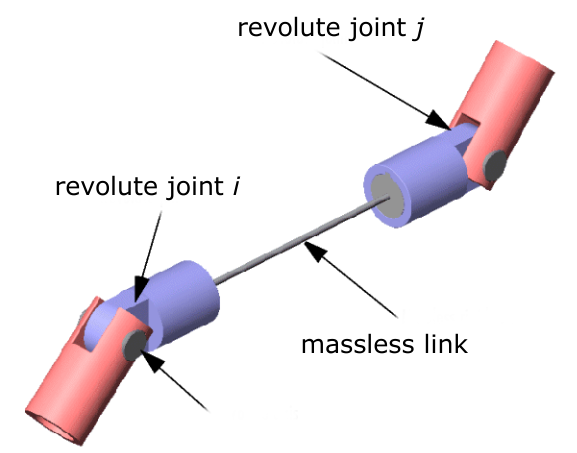
\includegraphics[width=0.5\linewidth]{images/kinematic_chains_1}
	\label{fig:kinematicchains1}
\end{figure}

\begin{figure}
	\centering
	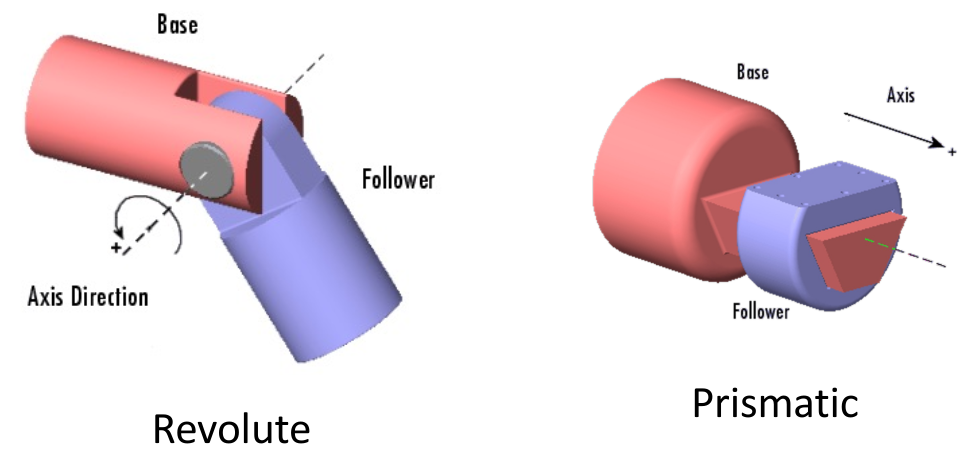
\includegraphics[width=0.6\linewidth]{images/kinematic_chains_2}
	\caption{Tipi di giunti}
	\label{fig:kinematicchains2}
\end{figure}

Noi analizzeremo solo \textbf{open chains} (in contrasto alle \textit{closed chains}): i.e. catene dove c'è solo 1 link fra due giunti qualunque. In questo caso la KC ha una struttura ad albero. Nel caso delle \textbf{closed chain}, invece, ci sono in generale più di un link fra due giunti e la struttura è ciclica.

I vari giunti sono schematizzati come mostrato in fig. \ref{fig:kinematicchains3}.

\begin{figure}[H]
	\begin{subfigure}{\linewidth}
		\centering
		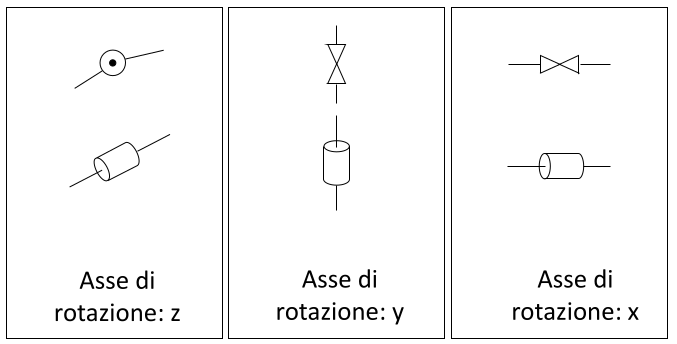
\includegraphics[width=0.6\linewidth]{images/kinematic_chains_3}
		\caption{Giunti rotoidali}
	\end{subfigure}
	\begin{subfigure}{\linewidth}
		\centering
		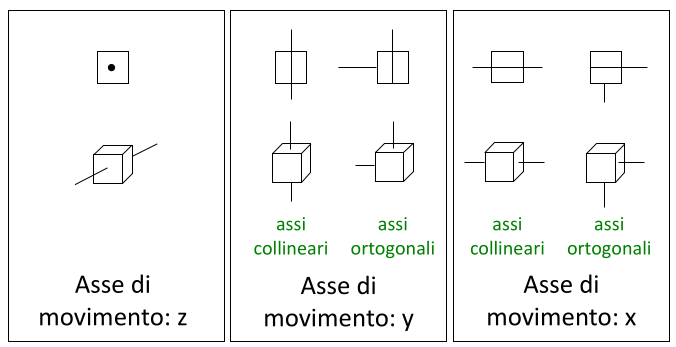
\includegraphics[width=0.6\linewidth]{images/kinematic_chains_4}
		\caption{Giunti prismatici}
	\end{subfigure}
	\caption{}
	\label{fig:kinematicchains3}
\end{figure}





\subsubsection{End Effector}

Oltre al braccio, un robot solitamente ha un \textit{tool} posto all'estremità (ultimo link). Questo è chiamato \textbf{end effector}, \textbf{gripper} o semplicemente \textbf{end tool}.

Il \textbf{TCP} (\textit{Tool Center Point}) è quel punto ideale sul'end-effector che i software muoveranno nello spazio. Come i vari giunti/link anche questo ha un proprio RF.

\begin{figure}
	\centering
	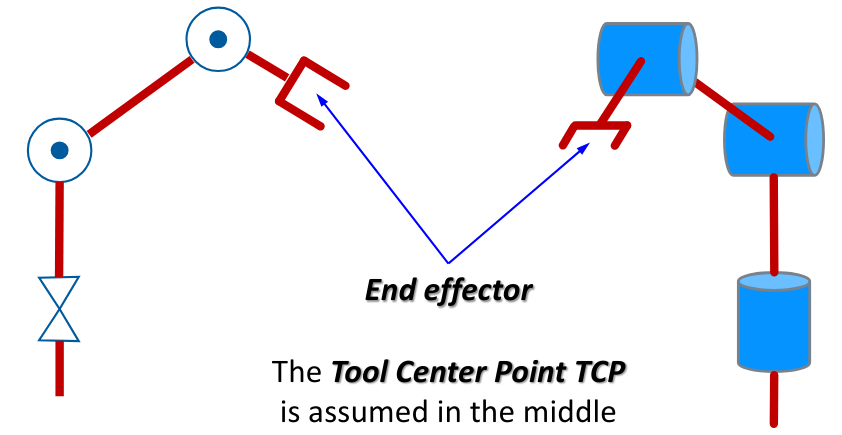
\includegraphics[width=0.6\linewidth]{images/kinematic_chains_5}
	\caption{Braccio robotico schematizzato}
	\label{fig:kinematicchains5}
\end{figure}



\section{Tipi di robot}

I robot industriali sono solitamente composti da una \textbf{shoulder} e un \textbf{wrist} (spalla e polso). Ponendo per notazione: P = "prismatic joint", R = "revolute joint". Di seguito i vari tipi, con le configurazioni delle relative shoulders.

\subsection{Possibili shoulder configurations}

\subsubsection{Cartesian}
\textbf{3P = P-P-P}: abbiamo 3 DoF, corrispondenti alle 3 coordinate cartesiane. Il \textit{task space} è un parallelepipedo. Posizionamento accurato ma desterità limitata.
\begin{figure}[H]
	\centering
	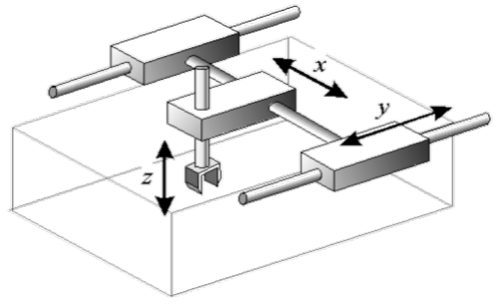
\includegraphics[width=0.35\linewidth]{images/kinematic_chains_6}
\end{figure}


\subsubsection{Cylindrical}	
\textbf{1R-2P = R-R-P}. Abbiamo 3 DoF, corrispondenti alle 3 coordinate cilindriche. Il \textit{task space} è una sezione di cilindro.\\
La stuttura essendo meno rigida rispetto al precedente ci da meno accuratezza (che va a diminuire con l'elongazione del braccio).

\begin{figure}[H]
	\begin{subfigure}{0.5\linewidth}
		\centering
		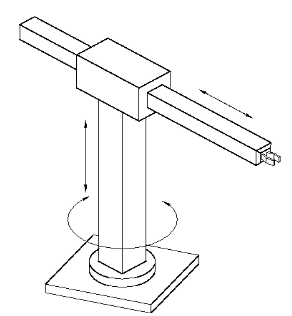
\includegraphics[width=0.4\linewidth]{images/kinematic_chains_7}
		\label{fig:kinematicchains7}
	\end{subfigure}
	\begin{subfigure}{0.5\linewidth}
		\centering
		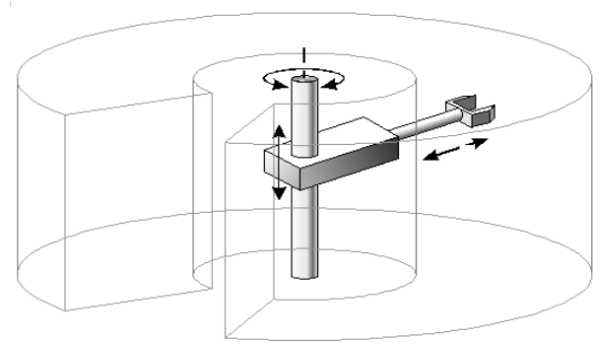
\includegraphics[width=0.65\linewidth]{images/kinematic_chains_16}
		\label{fig:kinematicchains16}
	\end{subfigure}
\end{figure}
	
\subsubsection{Polar or spherical}
\textbf{2R-1P = R-R-P}. Abbiamo 3 DoF, corrispondenti alle 3 coordinate polari. Il \textit{task space} è una sezione di una sfera. È ancora meno rigido rispetto alle precedenti (e come nel caso cilindrico l'accuratezza diminuisce con l'elongazione).
	
\begin{figure}[H]
	\centering
	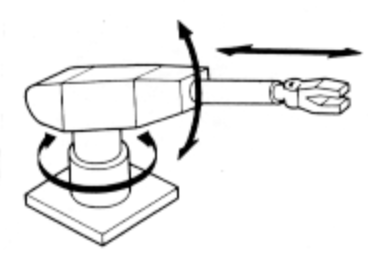
\includegraphics[width=0.25\linewidth]{images/kinematic_chains_10}
	\label{fig:kinematicchains10}
\end{figure}
	

\subsubsection{SCARA}
\textbf{2R-1P = R-R-P}. SCARA = Selective Compliance Assembly Robot Arm). Utili per manipolare piccoli componenti (e.g. $\mu$C). Abbiamo una corrispondenza fra DoM (degree of motion) e coordinata cartesiana solo per la componente verticale. L'effetto della gravità è compensato dalla struttura stessa, che è rigida verticalmente ma \textit{compliant} orizzontalmente.

\begin{figure}[H]
	\begin{subfigure}{0.5\linewidth}
		\centering
		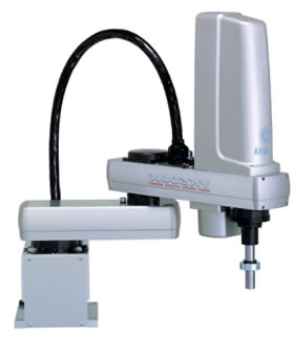
\includegraphics[width=0.4\linewidth]{images/kinematic_chains_8}
		\label{fig:kinematicchains8}
	\end{subfigure}
	\begin{subfigure}{0.5\linewidth}
		\centering
		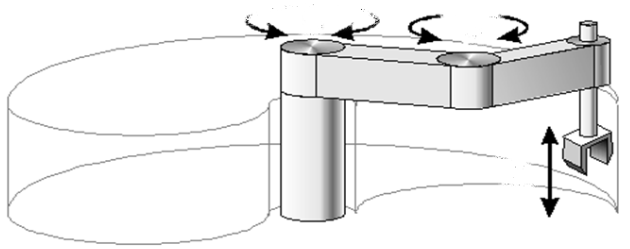
\includegraphics[width=0.7\linewidth]{images/kinematic_chains_15}
		\label{fig:kinematicchains15}
	\end{subfigure}
\end{figure}


\subsubsection{Articulated or Anthropomorphic}
\textbf{3R = R-R-R}. Simile ad un braccio umano. Non c'è corrispondenza fra giunti e coordinate cartesiane. Il \textit{task space} è una specie di sezione di una sfera. L'accuratezza non è costante in tutto il task-space. \textbf{È la tipologia più comune} visto che ci da la migliore desterità.

\begin{figure}[H]
	\centering
	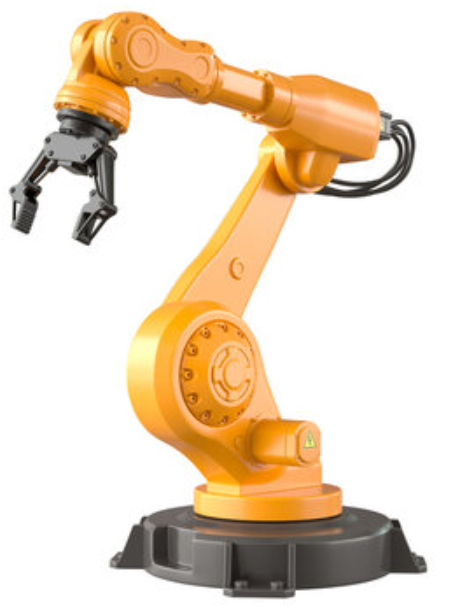
\includegraphics[width=0.15\linewidth]{images/kinematic_chains_9}
	\label{fig:kinematicchains9}
\end{figure}


\subsubsection{Parallel or closed chains}
Utili per manipolare payload pesanti, visto che questo tipo di struttura è molto rigida.

\begin{figure}[H]
	\begin{subfigure}{0.5\linewidth}
		\centering
		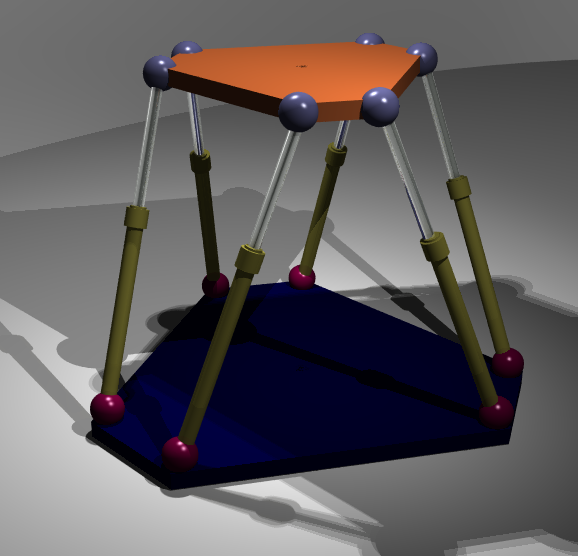
\includegraphics[width=0.3\linewidth]{images/kinematic_chains_11}
		\label{fig:kinematicchains11}
	\end{subfigure}
	 \hfill
	\begin{subfigure}{0.5\linewidth}
		\centering
		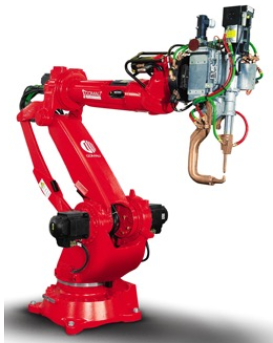
\includegraphics[width=0.3\linewidth]{images/kinematic_chains_12}
		\label{fig:kinematicchains12}
	\end{subfigure}
\end{figure}





\subsection{Wrist}
Lo scopo principale del polso è quello di orientare il TCP. Possiamo dire che la shoulder setta l'origine del TCP mentre il polso la sua orientazione.\\
La tipologia più comune è quello dello \textbf{spherical wrist}. Comunemente un wrist (sferico e non) è \textbf{composto da 3 rotational joints}.

\begin{figure}[H]
	\begin{subfigure}{0.6\linewidth}
		\centering
		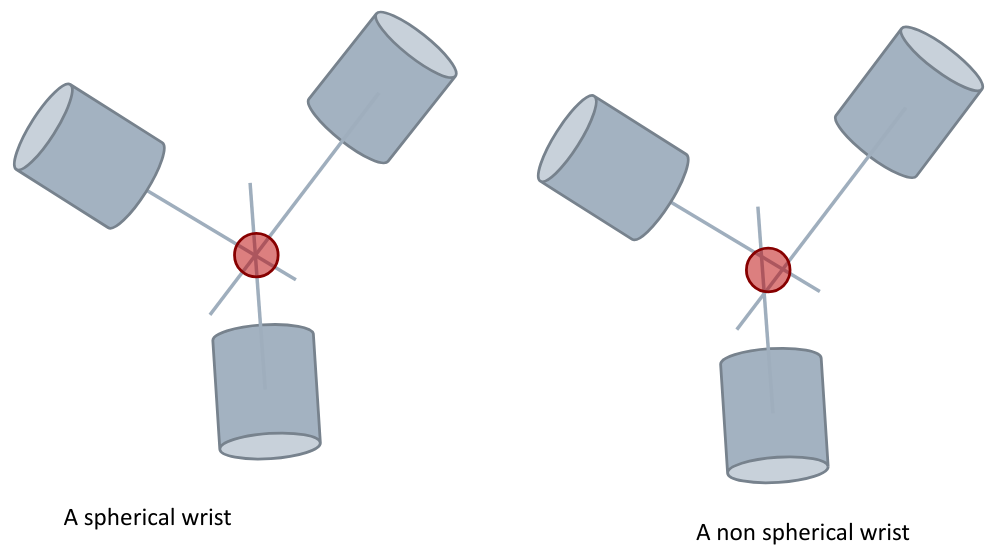
\includegraphics[width=0.8\linewidth]{images/kinematic_chains_13}
		\caption{Spherical vs non-spherical}
		\label{fig:kinematicchains13}
	\end{subfigure}
	\hfill
	\begin{subfigure}{0.4\linewidth}
		\centering
		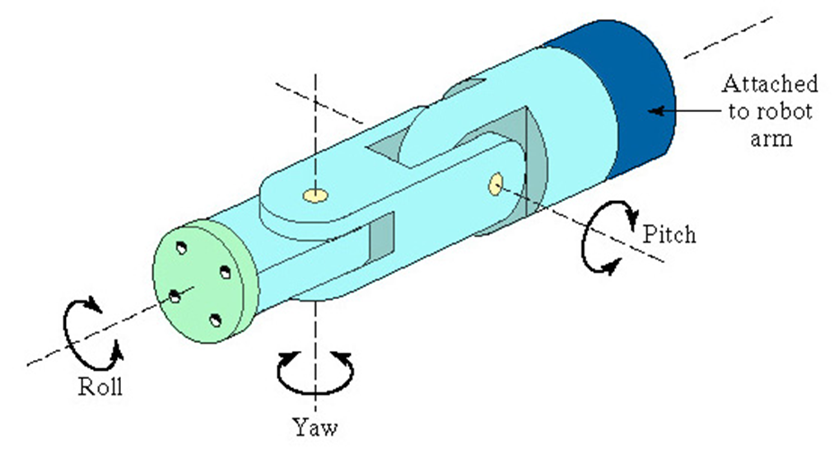
\includegraphics[width=0.9\linewidth]{images/kinematic_chains_14}
		\caption{Esempio}
		\label{fig:kinematicchains14}
	\end{subfigure}
\end{figure}






\chapter{Cinematica dei Robot}

In questo capitolo studieremo il metodo geometrico per ottenere la posizione dell'end-effector a partire dalle joint variables (angoli o posizioni). Notare che qua non consideriamo forze e coppie.
\vspace*{5pt}
\begin{figure}[H]
	\centering
	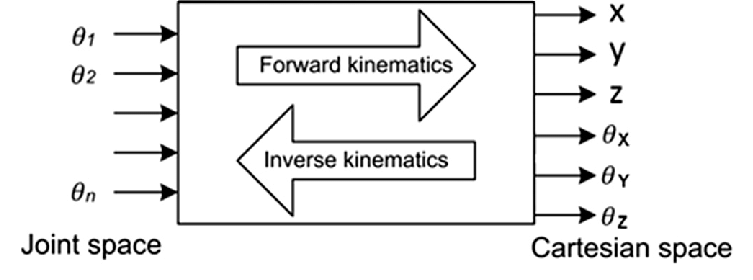
\includegraphics[width=0.5\linewidth]{images/kinematics_1}
	\label{fig:kinematics1}
\end{figure}


\section{Cinematica Diretta}

Sia $\mathcal{R}_b$ il \textbf{base frame} solidale con la base del robot, e sia $\mathcal{R}_e$ un sistema di riferimento mobile solidale con la punta operativa (end-effector) del robot.
Di conseguenza, la posa dell'end-effector sarà data dalla posizione ed orientamento di $\mathcal{R}_e$ rispetto a $\mathcal{R}_b$.

La cinematica diretta ha come scopo il calcolo della posa della punta operativa in funzione delle variabili giunto $q_i$, quindi dobbiamo esprimere la relazione fra i 2 RF in modo analitico.
Possiamo osservare che $\mathcal{R}_e$ può essere può essere rappresentato nel base frame $\mathcal{R}_b$ per mezzo della matrice di trasformazione:
$$
{}^b\textbf{T}_e(\mathbf{q}) = 
\begin{bmatrix}
	{}^b\mathbf{R}_e(\mathbf{q}) & {}^b\textbf{p}_e(\mathbf{q}) \\
	\mathbf{0} & 1
\end{bmatrix}
=
\begin{bmatrix}
	{}^b\mathbf{n}_e(\mathbf{q}) &
	{}^b\mathbf{s}_e(\mathbf{q}) & 
	{}^b\mathbf{a	}_e(\mathbf{q}) & 
	{}^b\textbf{t}_e(\mathbf{q}) \\
	0 & 0 & 0 & 1
\end{bmatrix}
$$
dove:
\begin{itemize}
	\item ${}^b\textbf{p}_e(\mathbf{q})$ è l'origine di $\mathcal{R}_e$ in $\mathcal{R}_b$
	\item ${}^b\mathbf{R}_e(\mathbf{q})$ è la matrice di rotazione di $\mathcal{R}_e$ rispetto a $\mathcal{R}_b$
	\item $	{}^b\mathbf{n}_e(\mathbf{q}), {}^b\mathbf{s}_e(\mathbf{q}), {}^b\mathbf{a	}_e(\mathbf{q})$ sono i 3 versori del sistema di riferimento dell'end-effector $\mathcal{R}_e$ (rispettivamente \textbf{approach}, \textbf{sliding} e \textbf{normal}).
\end{itemize}

Il nome dei 3 versori deriva dal fatto che:
\begin{itemize}
	\item approach: posizionato nella direzione di approccio dell’utensile al pezzo
	\item sliding: posizionato nel piano di scorrimento (sliding) delle ganasce
	\item normal: ottenuto come prodotto vettoriale fra i primi due (e quindi normale a loro).
\end{itemize}

\begin{figure}[H]
	\begin{subfigure}{0.65\linewidth}
		\centering
		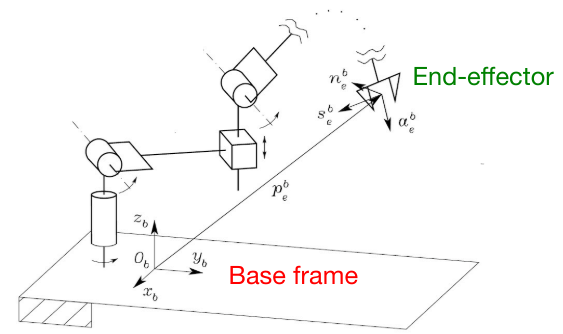
\includegraphics[width=0.9\linewidth]{images/kinematics_2}
		\caption{Esempio}
		\label{fig:kinematics2}
	\end{subfigure}
	\begin{subfigure}{0.3\linewidth}
		\centering
		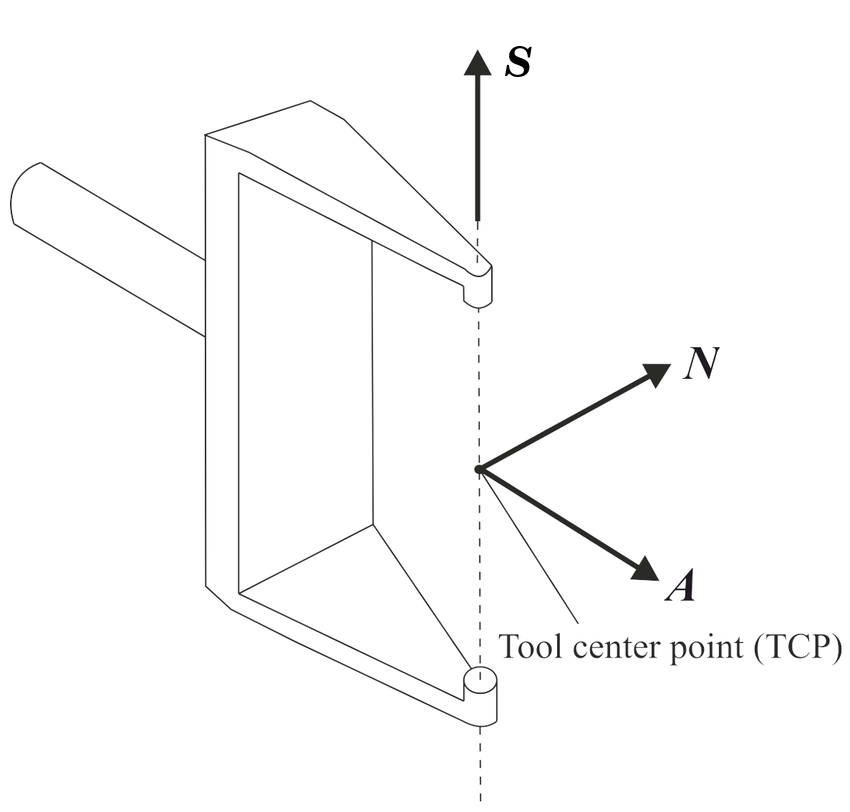
\includegraphics[width=1\linewidth]{images/kinematics_3}
		\caption{Versori di $\mathcal{R}_e$}
		\label{fig:kinematics3}
	\end{subfigure}
\end{figure}


Visto che
$$
\mathbf{x} = (x, y, z, \phi, \theta, \psi) = {}^b\textbf{T}_e(\mathbf{q})
$$
risolvere la cinematica diretta significa determinare trovare la matrice $\mathbf{T}$, che è specifica per ogni particolare robot (essendo dipendente dalla sua struttura fisica).


Soltanto nel caso di manipolatori estremamente semplici, con pochi gradi di libertà, è possibile risolvere il problema della cinematica diretta delle posizioni per via geometrica (i.e a manina). In generale, per un manipolatore con $n + 1$ links, collegati da $n$ giunti, è necessario ricorrere ad una procedura sistematica, basata su:
\begin{itemize}
	\item Definizione di $n + 1$ sistemi di riferimento $\mathcal{R}_0 \dots \mathcal{R}_n$ ciascuno solidale con un braccio del robot dalla base (braccio/link 0, $\mathcal{R}_0 \equiv \mathcal{R}_b$) fino all’ultimo braccio (n)
	\item Calcolo della matrice di trasformazione come prodotto (composizione) delle varie matrici di trasformazione fra i singoli sistemi di riferimento: 
	$$
	{}^b\textbf{T}_e(\mathbf{q}) \equiv {}^0\textbf{T}_n(\mathbf{q}) = 
	{}^b\textbf{T}_1(q_1)
	{}^1\textbf{T}_2(q_2)
	\cdots
	{}^{n-1}\textbf{T}_n(q_n)
	$$
\end{itemize}

\begin{figure}[H]
	\centering
	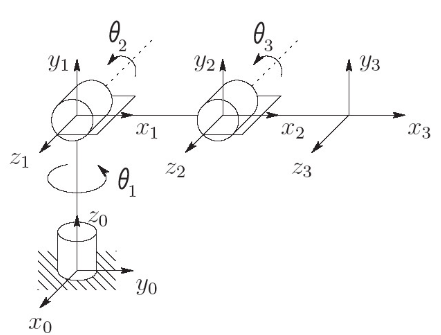
\includegraphics[width=0.5\linewidth]{images/kinematics_4}
	\caption{Sistemi di riferimento $\mathcal{R}_0 \dots \mathcal{R}_n$}
	\label{fig:kinematics4}
\end{figure}

Nota: la matrice $\mathbf{T(q)}$ \underline{non} è costante, ma dipende dalla configurazione corrente del robot!

Inoltre, se per qualche motivo la base e l'end effector non coincidono con i frame $0$ e $n$ ci basta aggiungere le 2 rispettive trasformazioni
$$
{}^b\textbf{T}_e(\mathbf{q}) =
{}^b\textbf{T}_0
{}^0\textbf{T}_n(\mathbf{q})
{}^n\textbf{T}_e
$$
che in generale sono costanti e non dipendono da $\mathbf{q}$.


\section{Convenzioni di Denavit-Hartenberg}
Queste convenzioni stabiliscono delle regole generali e sistematiche per la definizione dei sistemi di riferimento di ogni link. In particolare ci permettono di definire in maniera sistematica la matrice ${}^{i-1}\textbf{T}_i(q_i)$.

Se seguiamo le regole della convenzione (per il posizionamento dei RF), ogni matrice di quel tipo sarà funzione di soli 4 parametri:
\begin{itemize}
	\item $a_i$: lunghezza del link $i$
	\item $\alpha_i$: twist del link $i$
	\item $d_i$: offset del link $i$
	\item $\theta_i$: angolo del giunto $i$
\end{itemize}
Inoltre, visto che la matrice finale ${}^{i-1}\textbf{T}_i(q_i)$ è dipendente solo da una variabile ($q_i$), solo 1 fra quei 4 parametri potrà essere variabile, mentre gli altri saranno costanti. In particolare quelli variabili sono:
\begin{itemize}
	\item Se giunto rotoidale: $\theta_i = q_i$
	\item Se giunto prismatico: $d_i = q_i$
\end{itemize}


\subsection{Sistemi di riferimento}

\begin{figure}[b]
	\centering
	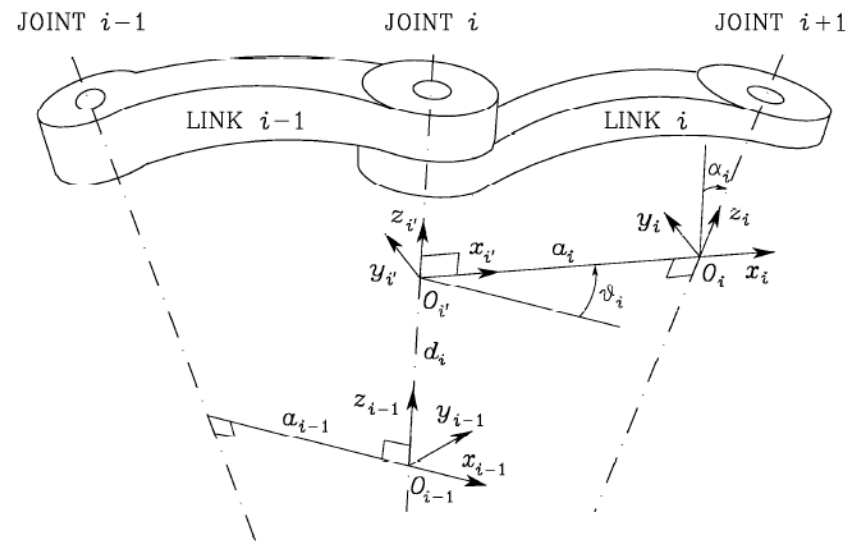
\includegraphics[width=0.6\linewidth]{images/kinematics_5}
	\caption{Convenzione di Denavit-Hartenberg}
	\label{fig:kinematics5}
\end{figure}

Introduciamo ora il metodo che dovremmo utilizzare per definire i vari RF. \\
In particolare vanno definiti $n + 1$ sistemi di riferimento $\mathcal{R}_i$, ognuno solidale con uno specifico braccio/link $i$ (importante notare che questo RF quindi si muoverà con quel particolare braccio, che a sua volta è attuato dal joint $i$)

Un ulteriore sistema di riferimento solidale con la punta operativa può essere introdotto, orientandone gli assi in maniera consona alla definizione del compito da svolgere.

\vspace*{25pt}
\textbf{Il sistema di riferimento $\mathcal{R}_i$ solidale con $\textit{LINK}_i$ viene definito secondo le seguenti regole\footnote{Notazioni slide italiano: $b_i \equiv \textit{LINK}_i \, \ g_i \equiv \textit{JOINT}_i$}:}\\

\circled{1} \textbf{Asse $z_i$ e origine $O_i$}
\begin{itemize}
	\item \textbf{L’asse} $\boldsymbol{z_i}$ è posto lungo l’asse di movimento di $g_{i+1}$ (asse di rotazione o di traslazione a seconda del tipo di giunto)
	\item \textbf{L’origine} $\boldsymbol{O_i}$ è posta all’intersezione di $z_i$ con la normale comune (\textit{common normal}) fra gli assi $z_{i-1}$ e $z_i$.
	La normale comune è quella retta perpendicolare ad entrambi gli assi (nota entrambi angoli retti nella figura)
	\item \textbf{Casi particolari}:
	\begin{itemize}
		\item $\boldsymbol{\mathcal{R}_0}$: qua è univocamente definita solo la direzione di $z_0$, data dall’asse di movimento di $g_1$; l’origine $O_0$ e $x_0$ possono essere fissati a piacimento
		\item $\boldsymbol{\mathcal{R}_n}$: visto che non esiste il giunto $g_{n+1}$, $z_n$ e $O_n$ non sono univocamente definiti. Per consuetudine si fissa l’origine nel centro della pinza. E visto che tipicamente l'ultimo giunto è rotoidale, $z_n$ è presa coincidente a a $z_{n-1}$ (così da semplificare la matrice di rotazione, visto che otterremo elementi nulli)
	\end{itemize}
\end{itemize}

\begin{figure}[H]
	\centering
	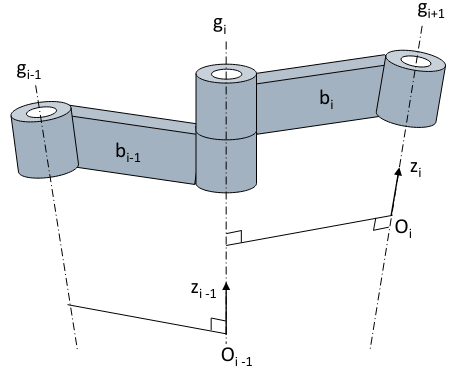
\includegraphics[width=0.4\linewidth]{images/kinematics_6}
	\caption{Assi $z$ e origini}
	\label{fig:kinematics6}
\end{figure}



\circled{2} \textbf{Asse $x_i$ e $y_i$}
\begin{itemize}
	\item \textbf{L’asse $\boldsymbol{x_i}$} è fissato lungo la normale comune fra gli assi $z_{i-1}$ e $z_i$
	\begin{itemize}
		\item Se $z_{i-1}$ e $z_i$ si intersecano, l’origine di $\mathcal{R}_i$ coincide con il loro punto di intersezione e la direzione di $x_i$ (ortogonale a $z_i$) è arbitraria
		\item se $z_{i-1}$ e $z_i$ sono paralleli, l’origine può essere posta in un punto a scelta e $x_i$ appartiene al piano normale a $z_{i-1}$ e $z_i$ con direzione e verso arbitrari 
	\end{itemize}
	\item \textbf{L’asse $\boldsymbol{y_i}$} completa la terna destrorsa
\end{itemize}


\begin{figure}[H]
	\centering
	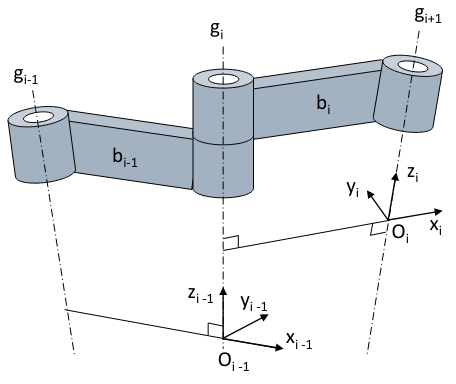
\includegraphics[width=0.4\linewidth]{images/kinematics_7}
	\caption{Assi $x$ e $y$}
	\label{fig:kinematics7}
\end{figure}



\circled{3} \textbf{Parametri di DH}\\
Per comprendere meglio i parametri di DH possiamo introdurre un sistema di riferimento "intermedio" $\mathcal{R}_{i'}$ (vedi fig. \ref{fig:kinematics9}):
\begin{itemize}
	\item $z_{i'}$ diretto lungo $z_{i-1}$
	\item $O_{i'}$ posta all’intersezione di $z_{i-1}$ con la normale comune fra $z_{i-1}$ e $z_i$
	\item $x_{i'}$ diretto lungo la normale comune fra	$z_{i-1}$ e $z_i$ (come $x_i$)
\end{itemize}

\setlength{\fboxsep}{7pt} % Adjust the padding as needed
\fbox{
	\begin{minipage}{\textwidth}
		La posizione e l’orientamento di $\mathcal{R}_i$ sono completamente specificati rispetto a $\mathcal{R}_{i-1}$ dai seguenti 4 parametri:
		\begin{itemize}
			\item $\boldsymbol{d_i} \rightarrow$ \textbf{link offset}: coordinata di $O_{i'}$ lungo $z_{i-1}$
			\item $\boldsymbol{\theta_i} \rightarrow$ \textbf{joint angle}: angolo di rotazione da $x_{i-1}$ a $x_i$ attorno all'asse $z_{i'}$ (positivo quando la rotazione è anti-oraria)
			\item $\boldsymbol{a_i} \rightarrow$ \textbf{link length}: distanza (con segno) fra $O_i$ e $O_{i'}$
			\item $\boldsymbol{\alpha_i} \rightarrow$ \textbf{link twist}: angolo di rotazione da $z_{i-1}$ a $z_i$ attorno all'asse $x_i$ (positivo quando la rotazione è anti-oraria)
		\end{itemize}
	\end{minipage}
}

\begin{figure}[H]
	\begin{subfigure}{0.5\linewidth}
		\centering
		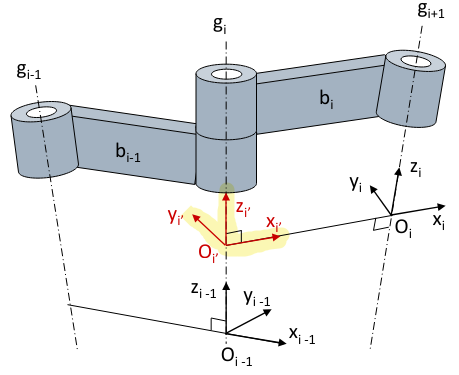
\includegraphics[width=0.95\linewidth]{images/kinematics_8}
		\caption{RF intermedio}
		\label{fig:kinematics8}
	\end{subfigure}
	\hfill
	\begin{subfigure}{0.5\linewidth}
		\centering
		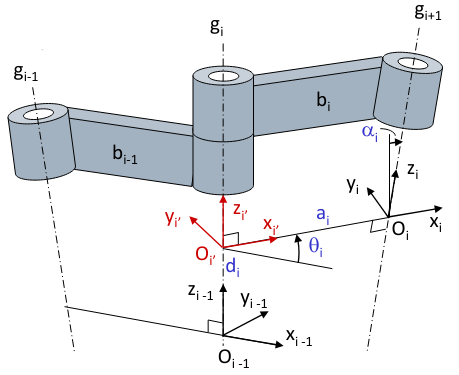
\includegraphics[width=0.95\linewidth]{images/kinematics_9}
		\caption{Parametri di DH}
		\label{fig:kinematics9}
	\end{subfigure}
	\caption{}
\end{figure}





\subsection{Trasformazione delle coordinate}
Ora, come possiamo usare questi parametri per ottenere $\mathbf{T(q)}$?\\


\circled{1} \boldmath$\mathcal{R}_{i-1} \rightarrow \mathcal{R}_{i'}$\unboldmath

$\mathcal{R}_{i'}$ (partendo da $\mathcal{R}_{i-1}$) è dato da una translazione $d_i$ lungo $z_{i-1}$ seguito da una rotazione di $\theta_i$ attorno a $z_i$, quindi:
$$
{}^{i-1}\mathbf{T}_{i'}
=
\begin{bmatrix}
	c\theta_i & -s\theta_i & 0 & 0 \\
	s\theta_i & c\theta_i & 0 & 0 \\
	0 & 0 & 1 & d_i \\
	0 & 0 & 0 & 1
\end{bmatrix}
$$


\vspace*{5pt}
\circled{2} \boldmath$\mathcal{R}_{i'} \rightarrow \mathcal{R}_{i}$\unboldmath

$\mathcal{R}_{i}$ (partendo da $\mathcal{R}_{i'}$) è dato da una translazione $a_i$ lungo $x_{i'}$ seguito da una rotazione di $\alpha_i$ attorno a $x_i$, quindi:
$$
{}^{i'}\mathbf{T}_{i}
=
\begin{bmatrix}
	1 & 0 & 0 & a_i \\
	0 & c\alpha_i & -s\alpha_i & 0 \\
	0 & s\alpha_i & c\alpha_i & 0 \\
	0 & 0 & 0 & 1
\end{bmatrix}
$$



\vspace*{5pt}
\circled{3} \boldmath$\mathcal{R}_{i-1} \rightarrow \mathcal{R}_{i}$\unboldmath

Infine, componendo le due trasformazioni, otteniamo:
$$
{}^{i-1}\mathbf{T}_{i}(q_i)
=
{}^{i-1}\mathbf{T}_{i'}
{}^{i'}\mathbf{T}_{i}
=
\begin{bmatrix}
	c\theta_i & -s\theta_ic\alpha_i & s\theta_is\alpha_i & a_ic\theta_i \\
	s\theta_i & c\theta_ic\alpha_i & -c\theta_is\alpha_i & a_is\theta_i \\
	0 & s\alpha_i & c\alpha_i & d_i \\
	0 & 0 & 0 & 1
\end{bmatrix}
$$

Quindi, per ottenere ${}^0\mathbf{T}_{n}(\mathbf{q})$ non ci basterà che comporre le varie matrici ottenute sopra, le quali possono essere facilmente ricavate inserendo i giusti valori dei 4 parametri.





\section{Operational space e Joint space}

L'\textbf{operational space (task space, o cartesian space)} è quello spazio dove è definito il vettore di posizioni e orientamento dell'end effector, ovvero:
$$
\boldsymbol{x}_e = (\boldsymbol{p}_e, \boldsymbol{\phi}_e) = (x, y, z, \phi, \theta, \psi)
$$

In contrasto, il \textbf{joint space (o configuration space)} è quello spazio dove è definito:
$$
\mathbf{q} = [q_1 \dots q_n] \in \mathbb{R}^n
$$
$q_i$ è la singola variabile di un giunto (ricordiamo che a ciascun giunto corrisponde un grado di libertà). In particolare:
\begin{itemize}
	\item Giunto rotoidale: $q_i = \theta_i$ (rotazione)
	\item Giunto prismatico: $q_i = d_i$ (traslazione)
\end{itemize}

La postura della catena cinematica è quindi determinata dalla posa di tutti i corpi rigidi (i bracci) che la costituiscono ed è una funzione di $\mathbf{q}$:
$$
\boldsymbol{x}_e 
= 
\begin{bmatrix}
	x(q_1, \dots, q_n) \\
	y(q_1, \dots, q_n) \\
	z(q_1, \dots, q_n) \\
	\phi(q_1, \dots, q_n) \\
	\theta(q_1, \dots, q_n) \\
	\psi(q_1, \dots, q_n) \\
\end{bmatrix}
= 
\boldsymbol{k}(\boldsymbol{q})
$$
dove $\boldsymbol{k}(\boldsymbol{q})$ è la \textbf{funzione di cinematica diretta}.

\textbf{Una soluzione} di questa funzione è data dalla matrice ${}^0\mathbf{T}_{n}(\mathbf{q})$ definita prima. Notiamo che però la soluzione trovata utilizza una rappresentazione non minimale dell'assetto (matrice di rotazione), mentre nella definizione di $k(q)$ è minimale (angoli di eulero).

\begin{figure}[!ht]
	\centering
	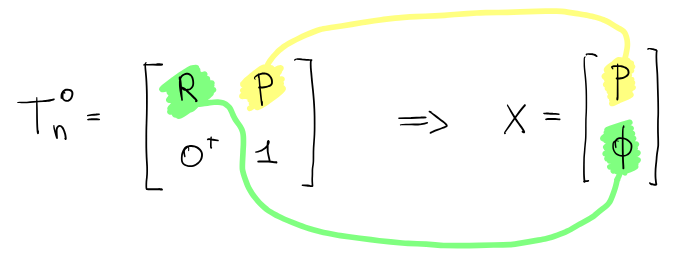
\includegraphics[width=0.6\linewidth]{images/kinematics_10}
	\caption{}
	\label{fig:kinematics10}
\end{figure}




\section{Workspace (spazio di lavoro)}
Con riferimento allo spazio operazionale lo \textbf{spazio di lavoro} del robot è definito da tutti quei punti di $\boldsymbol{x}_e$ ottenuti eseguendo tutte le possibili configurazioni dei giunti.
\begin{figure}[!bh]
	\centering
	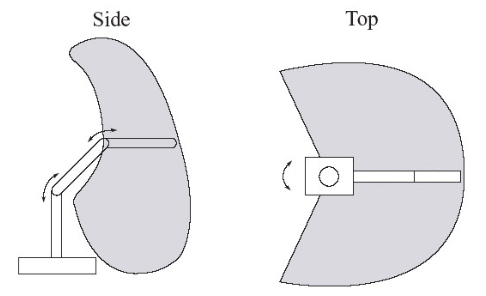
\includegraphics[width=0.5\linewidth]{images/kinematics_11}
	\caption{Esempio di spazio di lavoro}
	\label{fig:kinematics11}
\end{figure}

All'interno di questo spazio possiamo specificarne due:
\begin{itemize}
	\item \textbf{Reachable workspace}: è lo spazio di lavoro che l'end-effector può raggiungere con \underline{almeno un} orientamento
	\item \textbf{Dexterous workspace}: è lo spazio di lavoro che l'end-effector può raggiungere con \underline{più di un} orientamento. Ovviamente $\textit{dexterous workspace} \subset \textit{reachable workspace}$
\end{itemize}

Ad esempio, la punta di un manipolatore con meno di 6 gradi di libertà non può certamente raggiungere qualunque posa nello spazio 3D.





\section{Accuracy e Repeatability}

Per via di imprecisioni meccaniche, esisteranno sempre delle discrepanze fra i parametri DH nominali e quelli reali. Questa discrepanza prende il nome di \textbf{accuratezza}. Un requisito necessario per averla elevata è avere una struttura \textbf{rigida}.\\
Nei manipolatori moderni è $< 1$mm e solitamente varia con la posizione dell'end-effector.

La \textbf{repetibilità} invece è la capacità del manipolatore di ritornare ad una posizione precedente con un certo grado di precisione (questa dipende dalla struttura meccanica ma anche dalle strategie di controllo utilizzate e dalla precisione dei trasduttori).

\begin{figure}[!hb]
	\centering
	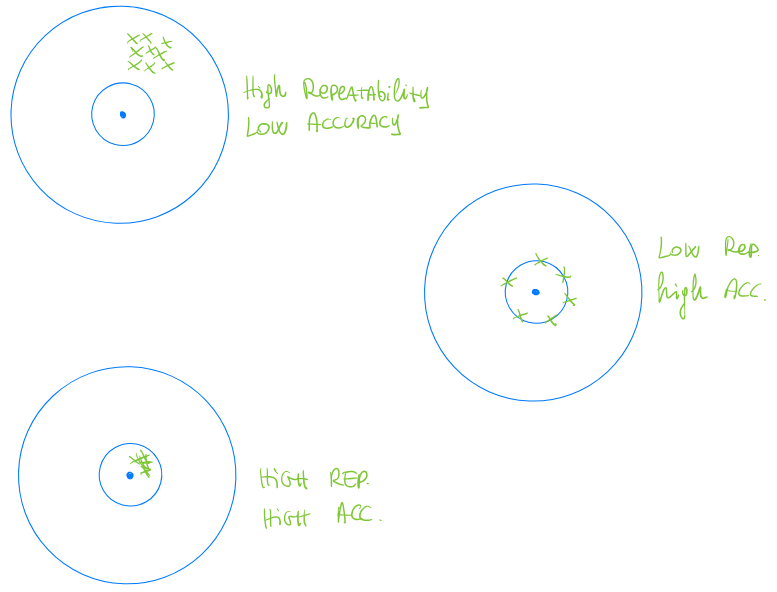
\includegraphics[width=0.6\linewidth]{images/kinematics_15}
	\caption{Esempi accuracy e repeatability}
	\label{fig:kinematics15}
\end{figure}




\section{Cinematica inversa}
Il problema della cinematica inversa delle posizioni consiste nella determinazione delle variabili giunto $\boldsymbol{q}$ corrispondenti ad un dato $\boldsymbol{x}_e$ o una data ${}^b\mathbf{T}_{e}(\mathbf{q})$.

L’esistenza della soluzione a tale problema è garantita solo se la posizione e l’orientamento della punta appartengono allo spazio di lavoro (di destrezza) del manipolatore.

Il \textbf{problema} della cinematica inversa delle posizioni è \textbf{molto più complesso} di quello della cinematica diretta: 
\begin{itemize}
	\item Le \textbf{equazioni} da risolvere sono in generale \textbf{non lineari} (a causa di $sin$, $cos$, ...) e di conseguenza non è sempre possibile trovare una soluzione in forma chiusa
	\item \textbf{Possono esistere molteplici soluzioni} (cioè più posture del manipolatore corrispondenti alla stessa posizione ed assetto della punta). Addirittura possono risultare infinite nel caso di un manipolatore ridondante
	\item \textbf{Possono anche non esistere proprio soluzioni}: vincoli cinematici nella struttura reale del robot potrebbero ridurre o azzerare il numero di soluzioni "ammissibili"
\end{itemize}

Putroppo \textbf{non esistono procedure} per il calcolo della cinematica inversa di un robot: la determinazione della soluzione in forma chiusa è fortemente basata su \textbf{intuizioni algebriche e geometriche}.\\
Nei casi in cui sia impossibile (o estremamente difficoltoso) giungere alla soluzione in forma chiusa si ricorre a \textbf{tecniche numeriche di soluzione}, ad esempio:
$$
\min_{q} = \| \boldsymbol{x}_{\text{e ref}} - \boldsymbol{k}(\boldsymbol{q}) \|
$$

Per quanto riguarda quest'ultime abbiamo come vantaggio che sono applicabili a qualunque struttura cinematica, ma che però non forniscono (in generale) tutte le possibili soluzioni.\\
Alternativamente è possibile utilizzare la \textbf{Jacobiana} (che vedremo più avanti), invertendo le velocità ed integrando per ottenere la posizione.



\subsection{Manipolatore con polso sferico}

Nel caso di un manipolatore a 6 DOF con polso sferico, \textbf{è possibile disaccoppiare} il problema della cinematica inversa in due sottoproblemi, relativi uno alla determinazione della posizione (del polso) e l’altro dell’assetto (dell'end-effector).\\
Indichiamo il centro del polso (inteso come la posizione in cui si intersecano gli assi dei suoi giunti) con $\boldsymbol{W}$.
\vspace*{-3pt}
\begin{figure}[H]
	\centering
	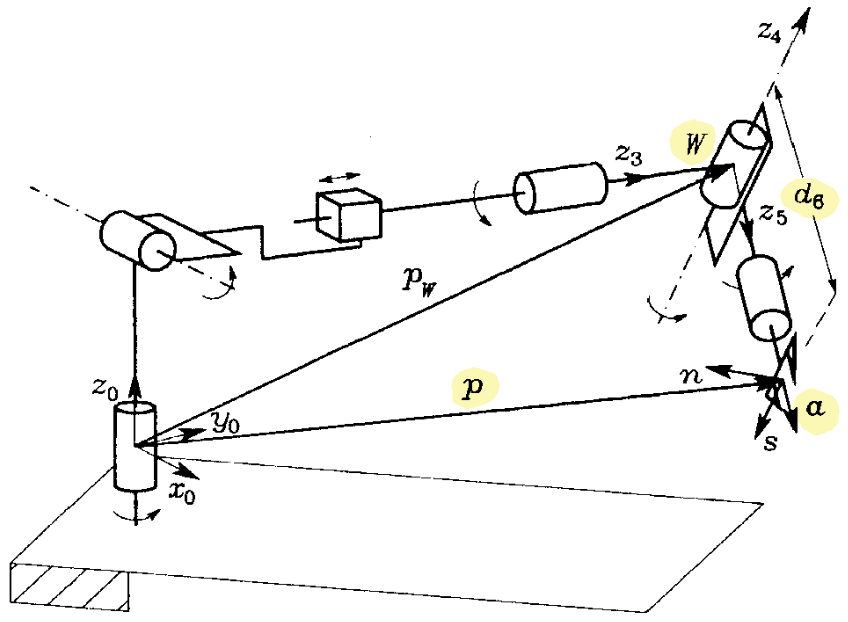
\includegraphics[width=0.5\linewidth]{images/kinematics_16}
	\label{fig:kinematics16}
\end{figure}

Se $\boldsymbol{p}$ e $\boldsymbol{(n,s,a)}$ (posizione e orientamento del polso) sono noti:
$$
\boldsymbol{W} = \boldsymbol{p} - d_6 \boldsymbol{a}
$$
poichè $W$, rappresentato dal vettore $p_W$, è ottenibile come sottrazione vettoriale fra $p$ e il vettore lungo $d_6$ orientato nel verso di $a$.

Grazie a questa osservazione, possiamo ora suddividere il problema della cinematica inversa in 2 parti:
\begin{enumerate}
	\item Dalla posizione $\boldsymbol{p}$ della punta è possibile ricavare $\boldsymbol{W}$ e quindi risolvere la cinematica inversa per determinare le tre variabili giunto "della spalla": calcola la posizione del polso $\boldsymbol{W}(q_1, q_2, q_3)$ tramite la formula sopra, e poi risolvi la cinematica inversa per $(q_1, q_2, q_3)$
	\item Tenendo conto della cinematica ormai nota della spalla, si passa al calcolo dei restanti $q_i$ a partire dall’assetto della punta: calcola ${}^0R_3(q_1, q_2, q_3) \implies {}^3R_6(\theta_1, \theta_2, \theta_3) = ({}^0R_3)^T \ {}^0	R_e$ e quindi risolvi la cinematica inversa per $(\theta_1, \theta_2, \theta_3)$ tramite ${}^3R_6$
\end{enumerate}
\chapter[Cinematica delle velocità]{Cinematica delle velocità \\ \large \textit{Differential Kinematics}}

La cinematica delle velocità (o cinematica differenziale) di un manipolatore è rappresentata dall’insieme di \textbf{relazioni che legano le velocità dei giunti alla velocità della punta operativa}, ovvero le relazioni fra la velocità nello spazio dei giunti e la velocità nello spazio operazionale.\\
Anche in questo caso abbiamo la relazione di cinematica diretta ($\dot{\boldsymbol{q}} \rightarrow \dot{\boldsymbol{x}}_e$) e di cinematica inversa ($\dot{\boldsymbol{q}} \leftarrow \dot{\boldsymbol{x}}_e$).

Mentre non ci sono ambiguità nella definizione della velocità nello spazio dei giunti, rappresentata dal vettore $\boldsymbol{\dot{q}}$ , è necessario chiarire che cosa si intende per velocità nello spazio operazionale:
\begin{itemize}
	\item \textbf{Velocità in senso geometrico}: si considera in tal caso il vettore $\boldsymbol{v} = (\boldsymbol{\dot{p}}, \boldsymbol{\omega}) \in \R^6$ delle velocità geometriche, formato dalla velocità lineare $\bm{\dot{p}} \in \R^3$ e dalla velocità angolare $\bm{\omega} \in \R^3$ della punta operativa
	\item \textbf{Velocità in senso analitico}: si definisce in tal caso come velocità nello spazio operazionale il vettore $\bm{\dot{x}}\in\R^6$ ottenuto derivando rispetto al tempo il vettore $\boldsymbol{x} = \bm{k}(\bm{q}) = (\boldsymbol{p}, \boldsymbol{\phi}) \in \R^6$ delle coordinate operazionali (determinate dalla cinematica diretta delle posizioni)
\end{itemize}


Notiamo che in entrambi i casi la parte lineare è identica (esprime la velocità lineare della punta operativa lungo le direzioni degli assi del sistema di riferimento $\mathcal{R}_0$). \textbf{La parte relativa all'orientamento}, invece, \textbf{differisce} (in generale $\bm{\omega} \neq \bm{\dot{\phi}}$):
\begin{itemize}
	\item $\bm{\omega}$ corrisponde alla velocità angolare della punta
	(secondo le tre componenti relative agli assi di $\mathcal{R}_0$). È un "vero" vettore: $\bm{\omega}(t) = \bm{\omega}_1(t) + \dots + \bm{\omega}_n(t)$
	\item $\bm{\dot{\phi}}$ rappresenta la velocità con cui varia l’orientamento della punta, espressa come derivata rispetto al tempo dei tre angoli $(\phi, \theta, \psi)$ (Eulero o RPY) della rappresentazione minima dell’assetto. A differenza di $\bm{\omega}$ questo non è un "vero" vettore, visto che $\bm{\phi}(t) \neq \bm{\phi}_1(t) + \dots + \bm{\phi}_n(t)$ ma (al contrario del precedente, essendo questa una derivata) $\int \bm{\dot{\phi}}(\tau) d\tau = \bm{\phi}(\tau)$
\end{itemize}
\ \\


In entrambi i casi i due vettori delle sono \textbf{funzioni lineari} delle velocità ai giunti, quindi:
\begin{align}
	\bm{v} &= \bm{J}(\bm{q})\dot{\bm{q}} \label{eq:geom_jacob} \\ 
	\bm{\dot{x}} &= \bm{J}_A(\bm{q})\dot{\bm{q}} \label{eq:analy_jacob}
\end{align}
dove le due matrici sono rispettivamente chiamate \textbf{Jacobiano geometrico} e \textbf{Jacobiano analitico}. Inoltre, per entrambe, posto $n=\text{numero giunti}$:
$$
\bm{J},\bm{J}_A \in \R^{6\times n}
$$

\textbf{Quindi, risolvere il problema della cinematica diretta delle velocità significa determinare $\bm{J}$ o $\bm{J}_A$}. \\
Importante notare anche che entrambi gli Jacobiani dipendono dalla configurazione corrente del robot, visto che sono funzioni di $\bm{q}$.




\section{Jacobiano geometrico}
Iniziamo studiando un modo per ricavare lo Jacobiano geometrico. Da (\ref{eq:geom_jacob}) richiamiamo:
\begin{equation}\label{eq:geom_jacob_2}
\bm{v} 
=
\begin{bmatrix*}
\dot{\bm{p}} \\
\bm{\omega}
\end{bmatrix*}
=
\bm{J}(\bm{q})\dot{\bm{q}} 
=
\begin{bmatrix*}
	\bm{J}_p(\bm{q}) \\
	\bm{J}_o(\bm{q}) 
\end{bmatrix*}
\dot{\bm{q}}
\end{equation}
dove abbiamo indicato la scomposizione dello Jacobiano nelle 2 sottomatrici $3\times n$ relative alla sola posizione e orientamento.

\begin{figure}[H]
	\centering
	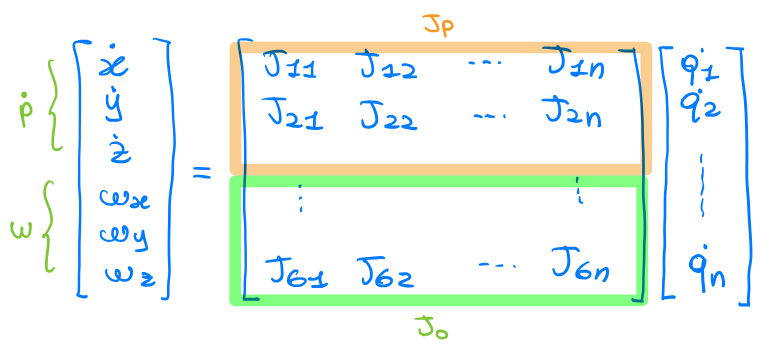
\includegraphics[width=0.6\linewidth]{images/diff_kine_1}
	\caption{Jacobiano geometrico}
	\label{fig:diffkine1}
\end{figure}
In primis possiamo iniziare osservando i contributi di ogni riga e ogni colonna:
\begin{itemize}
	\item \textbf{Righe}: ogni riga specifica l'effetto di \underline{tutti} i giunti sulla particolare velocità
	\item \textbf{Colonne}: ogni colonna, invece, identifica l'effetto del \underline{singolo} giunto su tutte le velocità
\end{itemize}

\vspace*{5pt}
\textit{\small Esempio:}\\
\textit{
\small
Se la colonna $i$ è completamente nulla, avremmo che il giunto $i$ \underline{non} avrà alcun effetto nella produzione di velocità dell'end-effector.\\
Invece se abbiamo una riga nulla, e.g. la $1^a$, avremmo che il nostro robot \underline{non} produrrà alcuna velocità (e quindi nessun movimento) lungo $x$.
}

\vspace*{5pt}
Anche dall'esempio possiamo intuire la grande utilità dello Jacobiano: \textbf{tramite questa matrice possiamo facilmente identificare quali velocità dei giunti influenzeranno maggiormente velocità operazionali}, oltre ad esempio, a rendere più facile l'inversione cinematica ($v = J(q)\dot{q} \implies \dot{q} = J^{-1}(q)v \implies q = \int \dot{q} = \int J^{-1}(q)v$), che vedremo più avanti.



\subsection{Costruzione dello Jacobiano geometrico}
Per comprendere come “"costruire" lo Jacobiano geometrico, è utile determinare l’espressione della velocità (lineare ed angolare) di un singolo braccio.\\
Si consideri il generico braccio $i$, facente parte di una catena cinematica aperta, per la quale sono stati definiti i sistemi di riferimento secondo le convenzioni di DH.

\begin{figure}[H]
	\centering
	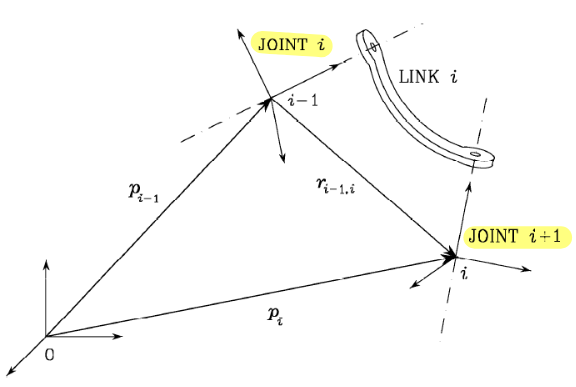
\includegraphics[width=0.5\linewidth]{images/diff_kine_2}
	\label{fig:diffkine2}
\end{figure}

Con riferimento alla figura sopra, possiamo affermare:
\begin{align*}
	\bm{\dot{p}}_i &= \bm{\dot{p}}_{i-1} + \bm{v}_{i-1, i} + \bm{\omega}_{i-1} \times \bm{r}_{i-1, i} \\
	\bm{\omega}_i &= \bm{\omega}_{i-1} + \bm{\omega}_{i-1, i}
\end{align*}
dove $\bm{v}_{i-1, i} \triangleq \bm{\dot{r}}_{i-1, i}$ (per dim. vedi slide in italiano).\\


Nel caso di un \textbf{giunto prismatico} abbiamo:
\begin{align*}
	\begin{cases}
		\bm{\omega}_{i-1,i} = 0 \\ 
		\bm{v}_{i-1, i} = \dot{\bm{d}}_i\bm{z}_{i-1}
	\end{cases}
	\implies
	\begin{cases}
		\bm{\dot{p}}_i = \bm{\dot{p}}_{i-1} + \dot{\bm{d}}_i\bm{z}_{i-1} + \bm{\omega}_{i-1} \times \bm{r}_{i-1, i} \\
		\bm{\omega}_i = \bm{\omega}_{i-1}
	\end{cases}
\end{align*}

mentre per un \textbf{giunto rotoidale}:
\begin{align*}
	\begin{cases}
		\bm{\omega}_{i-1,i} = \dot{\bm{\theta}}_i\bm{z}_{i-1} \\ 
		\bm{v}_{i-1, i} = \bm{\omega}_{i-1,i} \times \bm{r}_{i-1, i}
	\end{cases}
	\implies
	\begin{cases}
		\bm{\dot{p}}_i = \bm{\dot{p}}_{i-1} + \bm{\omega}_{i} \times \bm{r}_{i-1, i} \\
		\bm{\omega}_i = \bm{\omega}_{i-1} + \dot{\bm{\theta}}_i\bm{z}_{i-1}
	\end{cases}
\end{align*}

%Di conseguenza, richiamando (\ref{eq:geom_jacob_2}): $\begin{bmatrix*}\dot{\bm{p}} \\	\bm{\omega}\end{bmatrix*}=\bm{J}(\bm{q})\dot{\bm{q}}$ possiamo osservare che abbiamo trovato le due componenti di

Richiamando la fig. \ref{fig:diffkine1} e (\ref{eq:geom_jacob_2}), possiamo scomporre la matrice $\bm{J}$ come segue:
$$
\bm{J}(\bm{q})\dot{\bm{q}}
=
\begin{bmatrix*}
	\bm{J}_p(\bm{q}) \\
	\bm{J}_o(\bm{q}) 
\end{bmatrix*}
\dot{\bm{q}}
=
\begin{bmatrix*}
	\bm{J}_{p,1} & \bm{J}_{p,2} & \cdots & \bm{J}_{p,n} \\
	\bm{J}_{o,1} & \bm{J}_{o,1} & \cdots & \bm{J}_{o,n}
\end{bmatrix*}
\begin{bmatrix*}
	\dot{q}_1 \\ \dot{q}_2 \\ \vdots \\ \dot{q}_n
\end{bmatrix*}
$$
dove $\bm{J}_{p,i}$, $\bm{J}_{o,i} \in \R^3$ sono le colonne di $\bm{J}_p$ e $\bm{J}_o$ (per semplicità di notazione abbiamo omesso la dipendenza da $q$). Da qui poi possiamo scrivere:
$$
\bm{\dot{p}} = \sum_{i=1}^n \bm{J}_{p,i} \dot{q}_i
\qquad , \qquad
\bm{\omega} = \sum_{i=1}^n \bm{\omega}_{i-1, i} = \sum_{i=1}^n \bm{J}_{o,i} \dot{q}_i
$$
e quindi:

\begin{itemize}
	\item Nel caso di un \textbf{giunto prismatico} ($q_i = d_i$):
	\begin{align*}
		\begin{cases}
			\bm{J}_{p,i}\dot{q}_i = \bm{v}_{i-1,i} = \dot{d}_i \bm{z}_{i-1} \\
			\bm{\omega}_{i-1, i} = 0
		\end{cases}
		\implies
		\begin{cases}
			\bm{J}_{p,i} = \bm{z}_{i-1} \\
			\bm{J}_{o,i} = \bm{0}
		\end{cases}
	\end{align*}
	\item Mentre per un \textbf{giunto rotoidale} ($q_i = \theta_i$):
	\begin{align*}
		\begin{cases}
			\bm{J}_{p,i}\dot{q}_i = \bm{v}_{i-1,i} = \bm{\omega}_{i-1,i} \times \bm{r}_{i-1,e} = \dot{\bm{\theta}}_i\bm{z}_{i-1} \times (\bm{p}_e - \bm{p}_{i-1}) \\
			\bm{\omega}_{i-1,i} = \dot{\bm{\theta}}_i\bm{z}_{i-1}
		\end{cases}
		\implies
		\begin{cases}
			\bm{J}_{p,i} = \bm{z}_{i-1} \times (\bm{p}_e - \bm{p}_{i-1}) \\
			\bm{J}_{o,i} = \bm{z}_{i-1}
		\end{cases}
	\end{align*}
\end{itemize}


\vspace*{10pt}
Riassumendo:

\setlength{\fboxsep}{0pt} % Adjust the padding as needed
\fbox{
	\begin{minipage}{\textwidth}
		\begin{align*}
			\text{i-th column of } \bm{J}
			=
			\begin{bmatrix}
				\bm{J}_{p,i} \\
				\bm{J}_{o,i}
			\end{bmatrix}
			=
			\begin{cases}
				\begin{bmatrix}
					\bm{z}_{i-1} \\
					\bm{0}
				\end{bmatrix}
				& \textit{for a \textbf{prismatic} joint}
				\vspace*{5pt}
				\\
				\begin{bmatrix}
					\bm{z}_{i-1} \times (\bm{p} - \bm{p}_{i-1}) \\
					\bm{z}_{i-1} 
				\end{bmatrix}
				& \textit{for a \textbf{revolute} joint}
			\end{cases}
		\end{align*}
		\vspace*{2pt}
	\end{minipage}
}



\vspace*{25pt}
\subsubsection{Costruzione pratica}
Nella pratica, per trovare i vettori della formula di cui sopra, possiamo fare delle osservazioni.

\begin{itemize}
	\item $\bm{z}_{i-1} = 3^{a} \text{ colonna di } {}^0\bm{R}_{i-1} = {}^0\bm{R}_{1} \cdots {}^{i-2}\bm{R}_{i-1}$.
	\item $\bm{p}_e = \text{primi 3 elementi dell'ultima colonna di } {}^0\bm{T}_n = {}^0\bm{T}_{1} \cdots {}^{n-1}\bm{T}_{}$
	\item $\bm{p}_{i-1} = \text{primi 3 elementi dell'ultima colonna di } {}^0\bm{T}_{i-1} = {}^0\bm{T}_{1} \cdots {}^{i-2}\bm{T}_{i-1}$
\end{itemize}

\vspace*{10pt}
\textit{Esempio}\\
\textit{Per semplicità non useremo il grassetto per i vettori e} $p \equiv p_e$. \textit{Come si vede dalla figura abbiamo tutti giunti rotoidali.}
\begin{figure}[H]
	\centering
	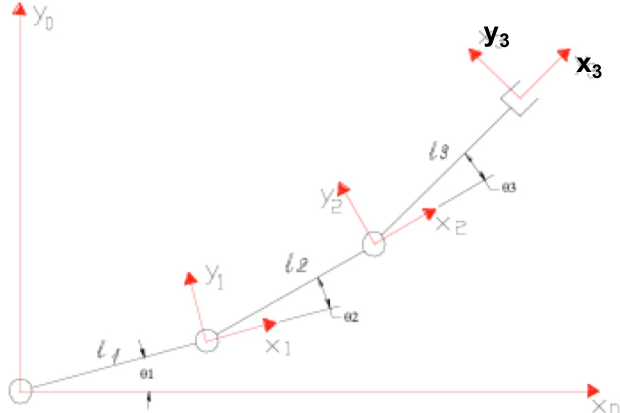
\includegraphics[width=0.4\linewidth]{images/diff_kine_3}
	\label{fig:diffkine3}
\end{figure}
$$
J(q)
=
\begin{bmatrix*}
z_0 \times (p - p_0) & z_1 \times (p - p_1) & z_2 \times (p - p_2) \\
z_0 & z_1 & z_2
\end{bmatrix*}
$$
\textit{e quindi}:
\begin{equation*}  
	{}^0T_0
	=
	\begin{bmatrix}
		1 & 0 & \cellcolor{cyan}0 & \cellcolor{yellow}0 \\
		0 & 1 & \cellcolor{cyan}0 & \cellcolor{yellow}0 \\
		0 & 0 & \cellcolor{cyan}1 & \cellcolor{yellow}0 \\
		0 & 0 & 0 & 1 \\
	\end{bmatrix}
	\implies
	\colorbox{cyan}{$z_0$}
	=
	\begin{bmatrix}
		0 \\ 0 \\ 1
	\end{bmatrix}
	\ , \
	\colorbox{yellow}{$p_0$}
	=
	\begin{bmatrix}
		0 \\ 0 \\ 0
	\end{bmatrix}
\end{equation*}

\begin{equation*}
	{}^0T_1
	=
	\begin{bmatrix}
		c_1 & -s_1 & \cellcolor{cyan}0 & \cellcolor{yellow}l_1 c_1 \\
		s_1 & c_1 & \cellcolor{cyan}0 & \cellcolor{yellow}l_1 s_1 \\
		0 & 0 & \cellcolor{cyan}1 & \cellcolor{yellow}0 \\
		0 & 0 & 0 & 1 \\
	\end{bmatrix}
	\implies
	\colorbox{cyan}{$z_1$}
	=
	\begin{bmatrix}
		0 \\ 0 \\ 1
	\end{bmatrix}
	\ , \
	\colorbox{yellow}{$p_1$}
	=
	\begin{bmatrix}
		l_1 c_1 \\ l_1 s_1 \\ 0
	\end{bmatrix}
\end{equation*}

\begin{equation*}
	{}^0T_2
	=
	\begin{bmatrix}
		c_{12} & -s_{12} & \cellcolor{cyan}0 & \cellcolor{yellow}l_1 c_1 + l_2c_{12}\\
		s_{12} & c_{12} & \cellcolor{cyan}0 & \cellcolor{yellow}l_1 s_1 + l_2s_{12}\\
		0 & 0 & \cellcolor{cyan}1 & \cellcolor{yellow}0 \\
		0 & 0 & 0 & 1 \\
	\end{bmatrix}
	\implies
	\colorbox{cyan}{$z_2$}
	=
	\begin{bmatrix}
		0 \\ 0 \\ 1
	\end{bmatrix}
	\ , \
	\colorbox{yellow}{$p_2$}
	=
	\begin{bmatrix}
		l_1 c_1 + l_2c_{12} \\ l_1 s_1 + l_2s_{12} \\ 0
	\end{bmatrix}
\end{equation*}

\begin{equation*}
	{}^0T_3
	=
	\begin{bmatrix}
		c_{123} & -s_{123} & 0 & \cellcolor{yellow}l_1 c_1 + l_2c_{12} + l_3c_{123}\\
		s_{123} & c_{123} & 0 & \cellcolor{yellow}l_1 s_1 + l_2s_{12} + l_3s_{123}\\
		0 & 0 & 1 & \cellcolor{yellow}0 \\
		0 & 0 & 0 & 1 \\
	\end{bmatrix}
	\implies
	\colorbox{yellow}{$p$}
	=
	\begin{bmatrix}
		l_1 c_1 + l_2c_{12} + l_3c_{123} \\ l_1 s_1 + l_2s_{12} + l_3s_{123} \\ 0
	\end{bmatrix}
\end{equation*}

\vspace*{10pt}
\textit{Ora dobbiamo solo calcolarci le differenze ed i prodotti vettoriali per trovare} $J(q)$:
\begin{figure}[H]
	\centering
	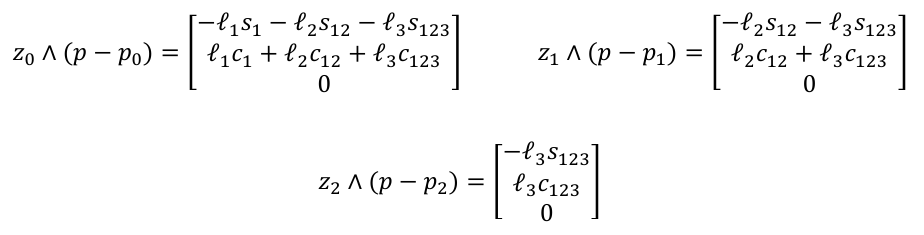
\includegraphics[width=0.8\linewidth]{images/diff_kine_4}
	\label{fig:diffkine4}
\end{figure}
\vspace*{-30pt}
$$
\Downarrow
$$
\begin{figure}[H]
	\centering
	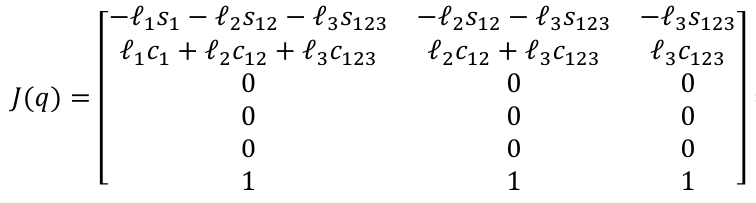
\includegraphics[width=0.6\linewidth]{images/diff_kine_5}
	\label{fig:diffkine5}
\end{figure}

\textit{In questo esempio possiamo già vedere l'esempio di un robot \textbf{sottoattuato}: a causa di tutti quegli 0 nella Jacobiana non possiamo controllare in alcun modo $\dot{z}, \omega_y, \omega_z$. In realtà in questo caso il risultato era atteso visto che abbiamo analizzato un manipolatore planare (2D) in 3D.\\ In questo caso è possibile utilizzare una rappresentazione ridotta di $J(q)$, levando le righe nulle (ovviamente bisogna ricordarci che è la versione ridotta)}.




\section{Jacobiano analitico}
Lo Jacobiano analitico viene calcolato dall’applicazione della sua stessa definizione, derivando rispetto al tempo il vettore $\bm{p}(\bm{q})$ ottenuto dalla cinematica diretta delle posizioni:	
\begin{gather*}
	\dot{\bm{x}}
	=
	\frac{d\bm{x}}{dt}
	=
	\underbrace{\frac{\partial\bm{x}}{\partial \bm{q}}}_{\bm{J}_A(\bm{q})}
	\underbrace{\frac{d\bm{q}}{d t}}_{\dot{\bm{q}}}
	=
	\bm{J}_A(\bm{q})\dot{\bm{q}}
\end{gather*}
E ${\partial\bm{x}} / {\partial \bm{q}}$ (che è proprio lo Jacobiano analitico) non è altro che lo Jacobiano (nel senso inteso ad analisi):
\[
\bm{J} = \frac{\partial \bm{f}}{\partial \bm{x}} =
\begin{bmatrix}
	\frac{\partial f_1}{\partial x_1} & \frac{\partial f_1}{\partial x_2} & \cdots & \frac{\partial f_1}{\partial x_n} \\[7pt]
	\frac{\partial f_2}{\partial x_1} & \frac{\partial f_2}{\partial x_2} & \cdots & \frac{\partial f_2}{\partial x_n} \\[5pt]
	\vdots & \vdots & \ddots & \vdots \\[5pt]
	\frac{\partial f_m}{\partial x_1} & \frac{\partial f_m}{\partial x_2} & \cdots & \frac{\partial f_m}{\partial x_n}
\end{bmatrix}
\]

\vspace*{10pt}
\subsubsection{Conversione $\bm{J}(\bm{q}) \leftrightarrow \bm{J}_A(\bm{q})$}
Data la rappresentazione minima prescelta per l’assetto (Eulero, RPY) è possibile esprimere $\bm{\omega}$ in funzione di $\dot{\bm{\phi}}$ come:
$$
\bm{\omega} = \bm{T}(\bm{\phi})\bm{\dot{\phi}}
$$
e quindi $\bm{J}(\bm{q})$ in funzione di $\bm{J}_A(\bm{q})$:
$$
\bm{J}(\bm{q})
=
\begin{bmatrix*}
\bm{I} & \bm{0} \\
\bm{0} & \bm{T}(\bm{\phi})
\end{bmatrix*}
\bm{J}_A(\bm{q})
$$
(la forma di $\bm{T}(\bm{\phi})$ dipende dalla rappresentazione scelta per l'assetto).

I valori di $\bm{\phi}$ per cui il determinante della matrice $\bm{T}(\bm{\phi})$ si annulla nei vari casi corrispondono a singolarità della rappresentazione dell’assetto usata (\textbf{gimbal lock}). Questo significa che ci sono velocità angolari che non possono essere espresse per mezzo di $\dot{\bm{\phi}}$.


\vspace*{5pt}
\textit{Esempio \\ Se prendiamo gli angoli di Eulero ZYZ}:
\begin{figure}[H]
	\centering
	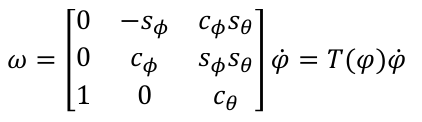
\includegraphics[width=0.4\linewidth]{images/diff_kine_6}
	\label{fig:diffkine6}
\end{figure}






\section{Singolarità cinematiche}
\textbf{Le configurazioni del manipolatore per cui lo Jacobiano (geometrico) non è di rango pieno sono dette singolarità cinematiche o configurazioni singolari}. Ovvero:
$$
\setlength{\fboxsep}{15pt}
\boxed{
\det(\bm{J}(\bm{q}_s)) = 0
\implies 
\bm{q}_s \text{ è una configurazione singolare}
}
$$

Le singolarità corrispondono a configurazioni in cui la mobilità del manipolatore è ridotta: 
\begin{itemize}
	\item Esistono velocità cartesiane che non possono essere ottenute da velocità ai giunti
	\item Velocità non nulle ai giunti generano velocità cartesiane nulle
\end{itemize}
Inoltre:
\begin{itemize}
	\item Quando il manipolatore è in configurazione singolare, il problema cinematico inverso può presentare infinite soluzioni
	\item In un intorno della singolarità, a piccole velocità della punta possono corrispondere grandi velocità dei giunti (poichè $v=J\dot{q} \implies \dot{q} = J^{-1}v \implies J^{-1} = \frac{1}{\det(J)} \text{adj}(J)$ e quindi se $\det(J) \to 0$ abbiamo $J^{-1} \to \infty$)
\end{itemize}

Le singolarità cinematiche possono essere:
\begin{itemize}
	\item \textbf{"di confine"}: i bracci del manipolatore sono completamente
	stesi o retratti, in una configurazione limite (“di confine”)
	dello spazio di lavoro
	\item \textbf{interne}: si trovano all’interno dello spazio di lavoro e
	corrispondono tipicamente all’allineamento di due o più assi
	di movimento dei giunti oppure a particolari configurazioni
\end{itemize}
Le configurazioni singolari interne sono le più critiche dal punto di vista pratico perché possono essere raggiunte ovunque all’interno dello spazio di lavoro durante l’esecuzione di una traiettoria pianificata nello spazio operazionale.


\subsection{Manipolatori con polso sferico}
Per i manipolatori con polso sferico le singolarità possono essere disaccoppiate in spalla e polso:
\begin{itemize}
	\item Per il \textbf{polso}, abbiamo singolarità quando 2 dei 3 assi si allineano, in particolare (con riferimento alla figura) $z_3$ e $z_5$. In generale, qualsiasi allineamento di due o più giunti rotanti porta ad una singolarità, poiché due rotazioni opposte di uguale entità non producono movimento nell'end-effector
	\begin{figure}[H]
		\centering
		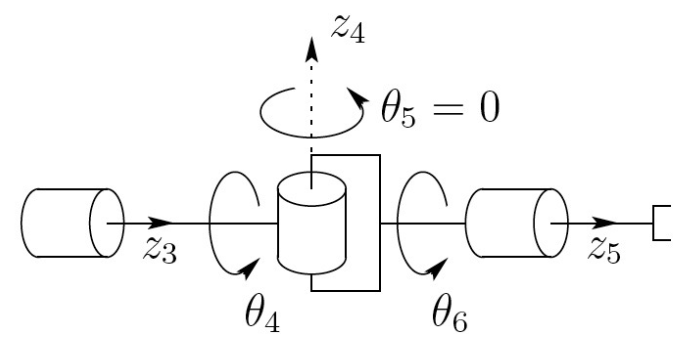
\includegraphics[width=0.35\linewidth]{images/diff_kine_7}
		\caption{Singolarità per $\theta_5 = 0, \pi$}
		\label{fig:diffkine7}
	\end{figure}
	\item Per la \textbf{spalla}, invece, possiamo analizzare le singolarità guardando il determinante di $\bm{J}_p$, che risulta nullo per $\theta_3=0,\pi$ (singolarità "di confine"):
	\begin{figure}[H]
		\centering
		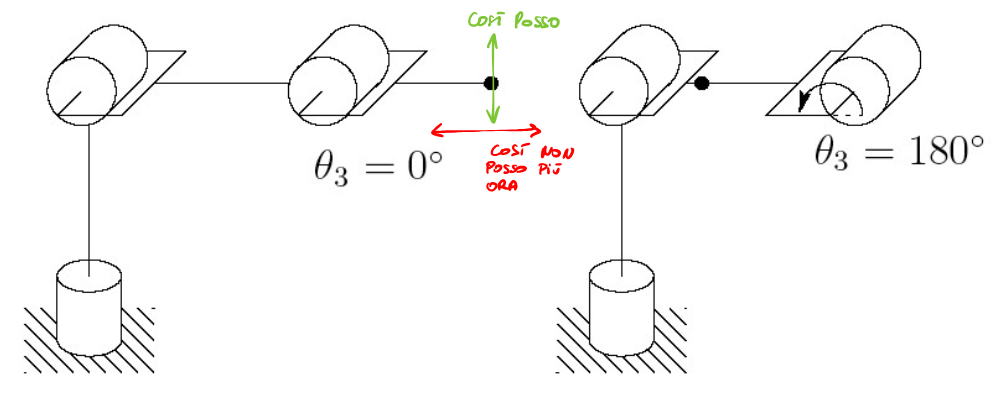
\includegraphics[width=0.4\linewidth]{images/diff_kine_8}
		\caption{Singolarità per $\theta_3=0,\pi$}
		\label{fig:diffkine8}
	\end{figure}
	oppure per $a_2c_2 + a_3c_{23}=0$ (singolarità interna):
	\begin{figure}[H]
		\centering
		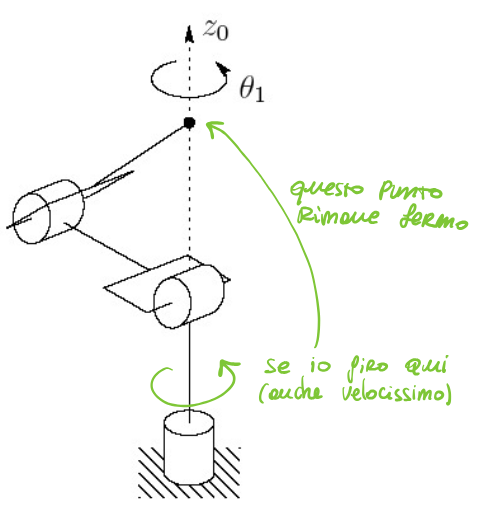
\includegraphics[width=0.35\linewidth]{images/diff_kine_9}
		\caption{Singolarità per $a_2c_2 + a_3c_{23}=0$}
		\label{fig:diffkine9}
	\end{figure}
	
\end{itemize}





\section{Ridondanza cinematica}

Un manipolatore è ridondante dal punto di vista cinematico se possiede un \textbf{numero di gradi di libertà maggiore del numero di variabili necessarie} per descrivere il compito che deve svolgere.

Un manipolatore è \textbf{intrinsecamente ridondante} se la dimensione $m$ del suo spazio operazionale è inferiore alla dimensione $n$ del suo spazio dei giunti. In generale, però, la ridondanza è un concetto relativo al compito assegnato al manipolatore (\textit{e.g. anche nel caso $m=n$ un manipolatore può risultare ridondante, come nel caso se per operare gli bastasse solo $x$ e $y$}).

Visto che $v = J(q)\dot{q}$ è un sistema lineare ($y = Ax$), possiamo analizzarlo utilizzando gli strumenti noti dell'algebra. Ricordiamo i seguenti concetti:
\begin{itemize}
	\item $\text{Im}(A) \equiv \text{span}(A) \equiv \mathcal{R}(A)$
	\item $\text{Ker}(A) \equiv \mathcal{N}(A) \triangleq \{ x : Ax = 0 \}$
	\item $A$ \textit{square} and $\det(A)\neq0 \iff \text{Ker}(A)=\{0\}$
	\item $A$ \textit{rectangular} $\implies \text{Ker}(A)\neq{\{0\}}$
\end{itemize}

Se un manipolatore è ridondante ($m > n$) abbiamo una matrice $J$ rettangolare:
$$
\bm{J}(\bm{q})
=
\begin{bmatrix}
	& & & & & & & & & \\
	& & & & & & & & & \\
\end{bmatrix}
=
\textit{rettangolare}
\implies
\text{Ker}(A)\neq{\{0\}}
$$
quindi, visto che il kernel \underline{non} è banale, da definizione avremo:
$$
\exists \bm{q} : \bm{J}(\bm{q}) = 0
$$ 
ovvero \textbf{esistono velocità dei giunti non nulle che non generano velocità nell'end-effector}.


\setlength{\fboxsep}{10pt} % Adjust the padding as needed
\fbox{
	\begin{minipage}{\textwidth}
		Da questa osservazione possiamo dire che:
		\vspace*{5pt}
		\begin{itemize}
			\item Il \textbf{range space} $\mathcal{R}(\bm{J}(\bm{q})) \in \R^m$ è quel sottospazio delle velocità dell'end-effector che possono essere generate da velocità ai giunti (per la postura corrente $\bm{q}$).
			\item Il \textbf{null space} $\mathcal{N}(\bm{J}(\bm{q})) \in \R^n$ è quel sottospazio delle velocità ai giunti che non producono alcuna velocità nell'end effector (per la postura corrente $\bm{q}$).
		\end{itemize}
	\end{minipage}
}


\vspace*{5pt}
\subsubsection{Altre cose dette da Rizzo}

Supponiamo $\dot{\bm{q}}^* \in \mathcal{N}(\bm{J}(\bm{q})) \implies \bm{J}(\bm{q})\dot{\bm{q}}^* = 0$. Allora, se poniamo $\bm{v} = \bm{J}(\bm{q})\dot{\bm{q}}$ abbiamo:
$$
\bm{v} = \bm{J}(\bm{q})(\dot{\bm{q}} + \dot{\bm{q}}^*) = \bm{J}(\bm{q})\dot{\bm{q}} + \cancelto{0}{\bm{J}(\bm{q})\dot{\bm{q^*}}} = \bm{J}(\bm{q})\dot{\bm{q}}
$$
Ora poniamo $\langle\dot{q}_1, \dot{q}_2, \dot{q}_3\rangle$ base di $\mathcal{N}(\bm{J}(\bm{q}))$. Grazie a questa terna, richiamando che ovviamente ora qualsiasi vettore ($\in \mathcal{N}(\bm{J}(\bm{q}))$) può essere scritto come $\alpha\dot{q}_1 + \beta\dot{q}_2 + \gamma\dot{q}_3$, possiamo definire:
$$
P \triangleq [ \dot{q}_1, \dot{q}_2, \dot{q}_3 ]
=
\text{matrice generatrice del null space}
$$
e quindi, qualsiasi $\dot{\bm{q}}^* \in \mathcal{N}(\bm{J}(\bm{q}))$ può essere scritto come:
$$
\dot{\bm{q}}^* = P\dot{q}_a \quad , \quad \dot{q}_a \text{ arbitrario}
$$






\section{Cinematica inversa delle velocità}
Il problema della cinematica inversa delle velocità consiste nel calcolo di $\dot{\bm{q}}$ partire dalla conoscenza di $\bm{v}$.

Se lo Jacobiano $\bm{J}(\bm{q})$ è \textbf{quadrato} e \textbf{full-rank}, il problema viene risolto semplicemente dall’equazione:
\begin{equation}\label{eq:diff_inv_kine}
\dot{\bm{q}} = \bm{J}^{-1}(\bm{q})\bm{v}
\end{equation}

Se, invece, siamo nel caso \textbf{rettangolare} e \textbf{non full-rank} (come nel caso di un manipolatore \textbf{ridondante}), dobbiamo trovare altri modi, ad esempio tramite la \textbf{right pseudo-inverse}:
\begin{align}\label{eq:diff_inv_kine_pseudo}
\dot{\bm{q}} = \bm{J}^{\dagger}(\bm{q})\bm{v}
\qquad
\textit{dove}
\qquad
\bm{J}^{\dagger} \triangleq \bm{J}^{T}(\bm{J} \bm{J}^{T})^{-1}
\end{align}


\subsection{Metodologie avanzate per il caso rettangolare/ridondante}
Soluzioni diverse possono essere ottenute ottimizzando la ricerca di $\dot{\bm{q}}$ con l’introduzione di opportuni funzionali di costo e di vincoli secondari, tali da permettere di sfruttare la ridondanza del manipolatore nell’esecuzione del compito.

Ad esempio:
\begin{align*}
\text{minimize} & \quad g(\dot{\bm{q}}) = \frac{1}{2} \dot{\bm{q}}^T \bm{W} \dot{\bm{q}} \\
\text{subject to} & \quad \bm{v} = \bm{J}(\bm{q})\bm{\dot{q}}
\end{align*}
dove $\bm{W}\in\R^{n\times n}$ è una matrice di pesi, simmetrica e definita positiva.\\
Tramite il metodo dei moltiplicatori di Lagrange (che ci permettono di includere il "subject to" dentro la funzione da minimizzare) possiamo ottenere una soluzione in forma chiusa per il problema dato:
$$
g(\dot{\bm{q}}, \lambda) = \frac{1}{2} \dot{\bm{q}}^T \bm{W} \dot{\bm{q}}
+ \lambda^T(\bm{v} - \bm{J}(\bm{q})\dot{\bm{q}})
$$
\begin{figure}[H]
	\centering
	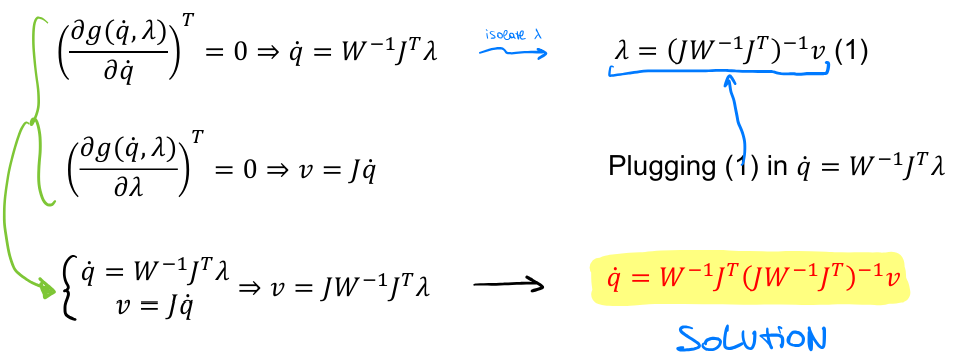
\includegraphics[width=0.7\linewidth]{images/diff_kine_10}
	\label{fig:diffkine10}
\end{figure}

Dove possiamo notare che ponendo $\bm{W} = \bm{I}$ questa soluzione è equivalente a quella con la pseudo-inversa destra.

Visto che lo Jacobiano rettangolare è relativo anche al caso di \textbf{manipolatori ridondanti}, nella nostra soluzione dovremmo tenere in considerazione le velocità non nulle dei giunti che non producono velocità dell'end-effector: riprendendo la soluzione (\ref{eq:diff_inv_kine_pseudo}), possiamo aggiungervi un qualsiasi vettore del null-space e rimarrà comunque valida:
\begin{equation*}
\dot{\bm{q}} = \bm{J}^{\dagger}(\bm{q})\bm{v}
+
\dot{\bm{q}}_n
\qquad
\textit{dove}
\qquad
\dot{\bm{q}}_n \in \mathcal{N}(\bm{J}(\bm{q}))
\tag{$\star$}
\end{equation*}
visto che l'ultimo termine è t.c. $\bm{J}(\bm{q})\dot{\bm{q}}_n = 0$:
$$
\bm{J}(\bm{q})
= 
\bm{J}(\bm{q})(\bm{J}(\bm{q})^{\dagger} \bm{v} + \bm{\dot{q}}_n)
=
\cancelto{I}{(\bm{J}(\bm{q}) (\bm{J}(\bm{q})^\dagger)} \bm{v} + \cancelto{0}{\bm{J}(\bm{q})\bm{\dot{q}}_n} = \bm{v}
$$

come scegliamo il vettore $\bm{\dot{q}}_n$? Possiamo usare un "trucco" accennato in precedenza: il \textit{proiettore} nel null space (prima chiamato matrice generatrice):
$$
\bm{J}^* = \bm{I} - \bm{J}^\dagger\bm{J}
$$
questa matrice "proietta" un qualsiasi vettore nel kernel, visto che $\bm{J}(\bm{J}^* \bm{\dot{q}}) = 0$, di conseguenza possiamo riscrivere $(\star)$ come:
\begin{equation}\label{eq:diff_inv_kine_redundant}
\boxed{
\dot{\bm{q}} = \bm{J}^{\dagger}(\bm{q})\bm{v}
+
(\bm{I} - \bm{J}^\dagger\bm{J})\dot{\bm{q}}_d
}
\end{equation}
che corrisponde alla soluzione in forma chiusa del problema:
\begin{align*}
	\text{minimize} & \quad 
	g'(\dot{\bm{q}}) = \frac{1}{2} ( \dot{\bm{q}} - \dot{\bm{q}}_d )^T ( \dot{\bm{q}} - \dot{\bm{q}}_d ) \\
	\text{subject to} & \quad \bm{v} = \bm{J}(\bm{q})\bm{\dot{q}}
\end{align*}
dove $\bm{\dot{q}}_d$ è un vettore di \textbf{velocità desiderate}: ovvero vogliamo $\bm{\dot{q}} \to \bm{\dot{q}}_d$. 

Da quest'ultima soluzione possiamo un'importante osservazione: \textbf{sfruttando i gradi di libertà in più, forniti dal manipolatore ridondante, riusciamo ad imporre velocità desiderate a dei giunti} (\textit{e.g. se voglio che il base joint vada molto lento, grazie alla ridondanza posso farlo}).




\subsection{Raggiungimento di obiettivi secondari}
Invece di impostare delle velocità desiderate per alcuni giunti, possiamo utilzzare i DoF "extra" per raggiungere altri obiettivi secondari.

Poniamo:
$$
\dot{\bm{H}}
=
\frac{d\bm{H}}{dt}
=
\frac{\partial\bm{H}}{\partial \bm{q}} \frac{d\bm{q}}{dt}
=
\frac{\partial\bm{H}}{\partial \bm{q}} \bm{\dot{q}}
=
\frac{\partial\bm{H}}{\partial \bm{q}} \bm{J}^{\dagger}(\bm{q})\bm{v}
+
\frac{\partial\bm{H}}{\partial \bm{q}}(\bm{I} - \bm{J}^\dagger\bm{J})\dot{\bm{q}}_d
$$
Ora vogliamo minimizzare $\bm{H}$, quindi dobbiamo far si che $\bm{\dot{H}} < 0$. Scegliamo:
\begin{gather*}
	\dot{\bm{q}}_d = -K(\frac{\partial\bm{H}}{\partial \bm{q}})^T \ , \ K > 0
\end{gather*}
così che:
$$
\dot{\bm{H}}
=
\underbrace{
\frac{\partial\bm{H}}{\partial \bm{q}} \bm{J}^{\dagger}(\bm{q})\bm{v}
}_{\text{non si sa}}
+
\underbrace{
-K\frac{\partial\bm{H}}{\partial \bm{q}}(\bm{I} - \bm{J}^\dagger\bm{J})(\frac{\partial\bm{H}}{\partial \bm{q}})^T
}_{<0}
$$

Variando $\bm{H}$ possiamo scegliere il nostro obiettivo secondario, di seguito alcune scelte tipiche:
\begin{itemize}
	\item \textbf{Massimizza distanza da ostacoli}: 
	\begin{itemize}
		\item $\displaystyle H = \min_{p,o} \| p(q) - o \| \qquad \rightarrow \text{massimizza } H$
		\item $p$: generico punto del manipolatore
		\item $o$: generico punto di un ostacolo
	\end{itemize}
	
	\item \textbf{Massimizza "distanza" dai limiti dei giunti}: 
	\begin{itemize}
		\item $\displaystyle H(q)=-{\frac{1}{2n}}\sum_{i=1}^{n}\left({\frac{q_{i}-{\bar{q}}_{i}}{q_{i M}-q_{i m}}}\right)^{2} \qquad \rightarrow \text{minimizza } H$ 
		\item ${\bar{q}}_{i}$: midpoint of the joint variable
		\item $q_{iM},q_{im}$: max and min excursion of the joint variable
	\end{itemize}
	
	\item \textbf{Massimizza "distanza" dalle singolarità}: 
	\begin{itemize}
		\item $H(q)=\sqrt{\operatorname*{det}(J(q)J^{T}(q))} \qquad \rightarrow \text{massimizza } H$ 
		\item In questo caso $H$ è chiamata misura di \textit{manipolabilità}
	\end{itemize}
\end{itemize}






\subsection{Inversione dello Jacobiano nel caso di singolarità}
Nel caso di singolarità abbiamo $\bm{J}$ non full-rank, di conseguenza invertire la matrice diventa più complesso. Ad esempio, in questo caso neanche la formula con la pseudo-inversa di (\ref{eq:diff_inv_kine_pseudo}) è applicabile, visto che anche $JJ^T$ è singolare e quindi non si può invertire ($\nexists \ (JJ^T)^{-1}$). Dobbiamo quindi trovare un modo alternativo per invertire lo Jacobiano.

Invece di utilizzare la pseudo-inversa, possiamo optare per un trade-off fra accuratezza e relizzabilità attraverso l'utilizzo del \textbf{damped-least-square}:
\begin{equation}\label{eq:damped_least_square}
\bm{J}^* = \bm{J}^T(\bm{J}\bm{J}^T + k^2\bm{I})^{-1}
\end{equation}

\begin{proof}
Partiamo dalla normale pseudo-inversa destra $J^\dagger = J^T(JJ^T)^{-1}$, quest'ultima può essere vista calcolata anche tramite la SVD di $J$:
$$
J^\dagger = V\Sigma^+ U^T
$$
dove
$$
\Sigma^{+}
=
\begin{bmatrix}
	\sigma_1^{-1} & & 0 \\
	& \ddots & \\
	0 & & \sigma_m^{-1}
\end{bmatrix}^T
$$
Il problema è che, nel caso di singolarità $1/q_i \to \infty$ (visto che $q_i \to 0$). Ora invece passiamo alla forma (\ref{eq:damped_least_square}), e calcoliamo anche questa tramite la SVD: l'unica differenza è nella matrice
$$
\Sigma^{+}
=
\begin{bmatrix}
	\frac{1}{\sigma_1 + k^2} & & 0 \\
	& \ddots & \\
	0 & & \frac{1}{\sigma_m + k^2}
\end{bmatrix}^T
$$
l'aggiunta del coefficiente $k^2$ permette di avere valori $\neq \infty$ anche quando $q_i \to 0$.
\end{proof}





\section{Cinematica inversa delle posizioni}
\subsection[section:invkineinvjac]{Cinematica inversa tramite Jacobiano inverso} \label{section:invkineinvjac}
Se la postura iniziale $\bm{q}(0)$ del robot è nota, \textbf{la cinematica inversa delle velocità può essere utilizzata per risolvere indirettamente il problema della cinematica inversa delle posizioni}, calcolando $\bm{q}(t)$ per integrazione
$$
v = J(q)\dot{q} \implies \dot{q} = J(q)^{-1}v \implies q = \int \dot{q} = \int J(q)^{-1}v
$$
ovvero:
\begin{figure}[H]
	\centering
	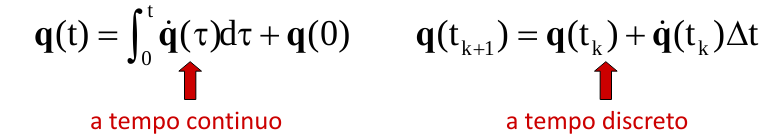
\includegraphics[width=0.7\linewidth]{images/diff_kine_11}
	\label{fig:diffkine11}
\end{figure}
e inserendo la forma di $\bm{q}$ ottenuta tramite lo Jacobiano (geometrico):
\begin{figure}[H]
	\centering
	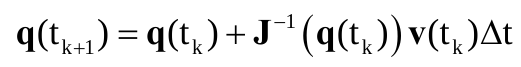
\includegraphics[width=0.4\linewidth]{images/diff_kine_12}
	\label{fig:diffkine12}
\end{figure}

Il problema con questa soluzione \textit{naïve} è che a causa di errori numerici divergeremo dalla soluzione voluta:
\begin{equation}\label{eq:inv_kine_diff_error}
\bm{e} = \bm{x}_d - \bm{x}
\end{equation}
Per risolvere il problema possiamo andare ad analizzare la dinamica d'errore:
\begin{equation*}
\bm{\dot{e}} = \bm{\dot{x}}_d - \bm{\dot{x}} = \bm{\dot{x}}_d - \bm{J}_A(\bm{q})\dot{\bm{q}}
\tag{$\star$}
\end{equation*}
e "chiudere il loop" per avere un feedback e correggere questo drift (e quindi far si che $\bm{e} \to 0$). Da qui, per semplicità supponendo che $\bm{J}_A$ sia invertibile, possiamo porre:
$$
\bm{\dot{q}}
\triangleq
\bm{J}_A^{-1}(\bm{q}) ( \dot{\bm{x}}_d + \bm{K}\bm{e})
$$
e, sostituendo in ($\star$), otteniamo la seguente dinamica d'errore:
\begin{gather*}
\bm{\dot{e}} = \bm{\dot{x}}_d - \bm{J}_A(\bm{q}) ( \bm{J}_A^{-1}(\bm{q}) ( \dot{\bm{x}}_d + \bm{K}\bm{e}) ) \\
\Downarrow \\
\bm{\dot{e}} = -\bm{K}\bm{e} \\
\Downarrow \\
\bm{\dot{e}} + \bm{K}\bm{e} = 0
\end{gather*}
dove se $\bm{K} > 0$ abbiamo stabilità asintotica dell'errore ($\implies \bm{x} \to \bm{x}_d$). Questa strategia può essere utilizzata per implementare il controllo cinematico, e funziona per basse velocità.

\begin{figure}[!hb]
	\centering
	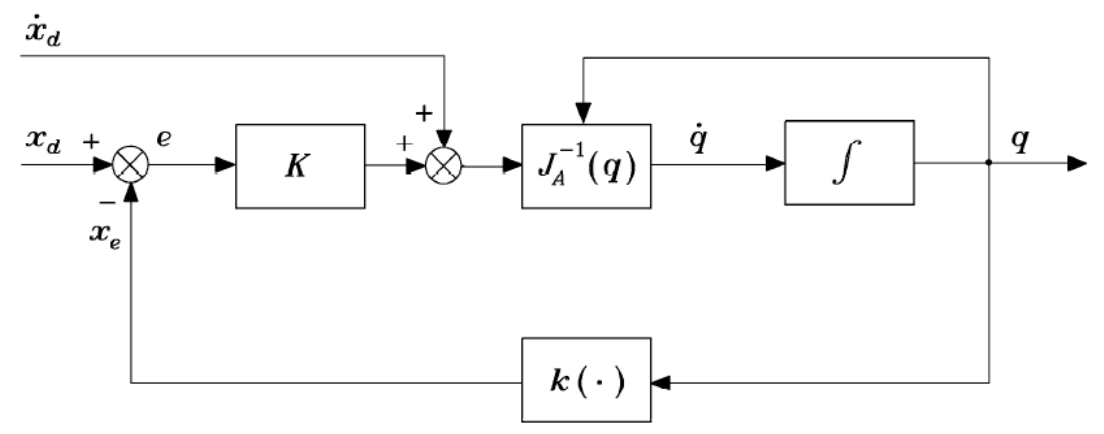
\includegraphics[width=0.7\linewidth]{images/diff_kine_13}
	\caption{Circuito di controllo con Jacobiano inverso e feedback}
	\label{fig:diffkine13}
\end{figure}




\subsection{Cinematica inversa tramite Jacobiano trasposto}
Nella soluzione tramite Jacobiano inverso stiamo in pratica usando una sorta di feedback linearization per trasformare la dinamica d'errore (non-lineare) in un'equazione lineare che possiamo facilmente controllare. Lo svantaggio principale di questa tecnica, è che richiede l'inversione di $\bm{J}(\bm{q})$, che (soprattutto nel di singolarità o ridondanza) è computazionalmente molto pesante.

Potremmo quindi pensare di progettare un "controllore" per l'errore direttamente nel caso non-lineare, ad esempio tramite il \textbf{metodo diretto di Lyapunov}. Scegliamo
$$
V(\bm{e})=\frac{1}{2}\bm{e}^{T}\bm{K}\bm{e} > 0 \quad \forall \bm{e} \neq \bm{0}
\qquad
,
\qquad
V(\bm{0}) = 0
$$
con $\bm{K} > 0$. Derivando e richiamando (\ref{eq:inv_kine_diff_error}), otteniamo:
$$
\dot{V}
=
\bm{e}^{T}\bm{K}\dot{\bm{x}}_{d} - \bm{e}^{T}\bm{K}\dot{\bm{x}}_{\bm{e}}
=
\bm{e}^{T}\bm{K}\dot{\bm{x}}_{d} - \bm{e}^{T}\bm{K} \underbrace{\bm{J}_A(\bm{q})\bm{\dot{q}}}_{\dot{\bm{x}}}
$$
e ponendo
$$
\dot{\bm{q}} \triangleq \bm{J}_{A}^{T}(\bm{q})\bm{K} \bm{e}
$$
otteniamo $\dot{V} < 0$ nel caso di riferimenti costanti ($\bm{x}_d = \text{const}$ i.e. $\bm{\dot{x}}_d = 0$).

\begin{figure}[!ht]
	\centering
	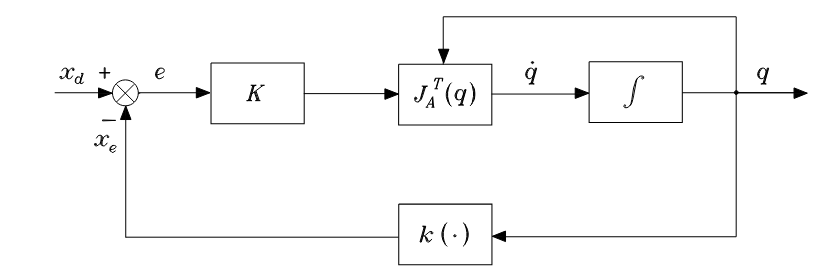
\includegraphics[width=0.7\linewidth]{images/diff_kine_14}
	\caption{Cinematica inversa con Jacobiano trasposto (riferimento costante)}
	\label{fig:diffkine14}
\end{figure}

Per il caso di $\bm{x}_d$ tempo-variante ($\bm{\dot{x}}_d \neq 0$), non riusciamo a garantire la convergenza dell'errore, che possiamo dire essere solo norm-bounded e inversamente proporzionale a $\bm{K}$. Per avere convergenza di tale errore dovremmo nuovamente scegliere $\dot{\bm{q}}$ dipendente dallo (pseudo-)inverso dello Jacobiano (quindi ritornando al caso di sez. \ref{section:invkineinvjac})
\chapter{Statica}

Obiettivo della statica è la \textbf{determinazione delle relazioni fra le forze e le coppie applicate sulla punta operativa e le forze e le coppie applicate ai giunti}, quando il manipolatore si trova in una \textbf{configurazione di equilibrio} (i.e. quando tutto è fermo).

Chiamiamo \textbf{forze generalizzate} il vettore composto di forze e coppie (torques) assieme (tecnicamente questo non sarebbe un vettore perchè gli elementi hanno unità di misure diverse: forze in $N$, coppie in $Nm$).

Indicheremo con
$$
\bm{F}
\triangleq
\begin{bmatrix*}
\bm{f}(t) \\
\bm{N}(t)
\end{bmatrix*}
\qquad
\bm{f},\bm{N} \in \R^3
$$
($f$ forze, $N$ momenti) il vettore delle \textbf{forze generalizzate cartesiane} applicate sulla punta operativa (task space generalized forces (\textbf{TSGF})), mentre con
$$
\bm{\tau}(t)
\triangleq
\begin{bmatrix*}
	\tau_1 \\
	\vdots \\
	\tau_n
\end{bmatrix*}
$$
il vettore delle \textbf{forze generalizzate ai giunti} (joint generalized forces (\textbf{JGF})); visto che i giunti maggiormente impiegati sono di tipo rotoidale, $\bm{\tau}(t)$ è spesso indicato come vettore delle \textbf{coppie generalizzate}.

\begin{itemize}
	\item Per \textbf{giunti prismatici}: 
	$$
	\tau_i = \bm{k}^T_{i-1} \bm{f}_{i-1,i}
	$$
	\item Per \textbf{giunti rotoidali}: 
	$$
	\tau_i = \bm{k}^T_{i-1} \bm{N}_{i-1,i}
	$$
\end{itemize}


Le TSGF sono generate dalle interazioni della punta con l'ambiente (e.g. quando il TCP preme contro una superficie), mentre le JGF sono generate dalla potenza sviluppata dai motori.

\begin{figure}[H]
	\centering
	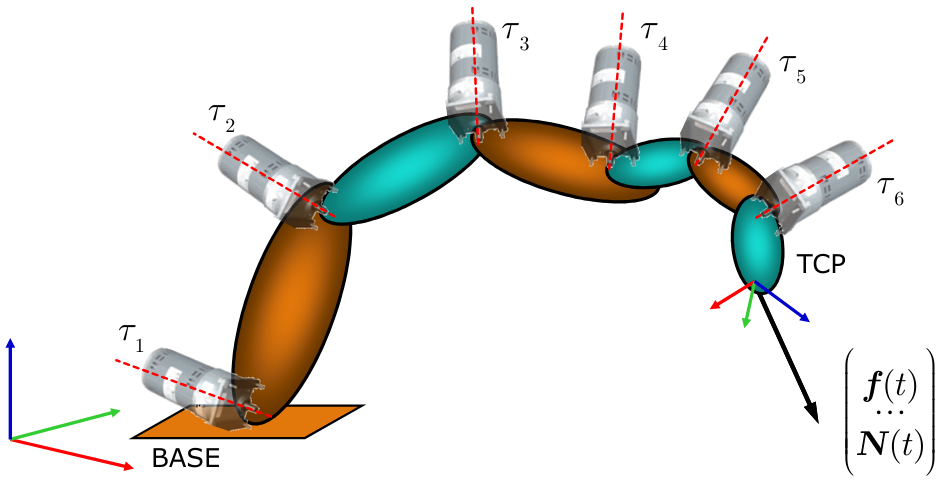
\includegraphics[width=0.7\linewidth]{images/statics_1}
	\caption{Statics}
	\label{fig:statics1}
\end{figure}

\section{Relazione fra $F$ e $\tau$}
Per trovare questa relazione possiamo usare il \textbf{principio dei lavori virtuali}:
\begin{itemize}
	\item Il \textbf{lavoro} è una grandezza reale data dal prodotto di una forza per uno spostamento lineare oppure dal prodotto di un momento per uno spostamento angolare
	\item Il \textbf{lavoro virtuale} è quello associato agli spostamenti virtuali, dati da tutti i possibili spostamenti geometrici compatibili con gli eventuali vincoli sul sistema
\end{itemize}
Il lavoro virtuale nasce dall'applicazione del \textbf{principio di minima azione} allo studio delle forze e del movimento di un sistema meccanico. Il lavoro di una forza che agisce su una particella mentre si muove lungo uno spostamento è diverso a seconda degli spostamenti. Tra tutti i possibili spostamenti che una particella può seguire, detti \textbf{spostamenti virtuali}, quello ne minimizzerà l'azione. Questo spostamento è quindi lo spostamento seguito dalla particella secondo il principio di minima azione. Il lavoro di una forza su una particella lungo uno spostamento virtuale è noto come lavoro virtuale.

Sia
$$
\delta W_{TCP} = \bm{F}^T\delta\bm{p}
$$
il lavoro virtuale associato alle forze generalizzate cartesiane, dove $\delta\bm{p}$ è lo spostamento virtuale cartesiano (formato dagli spostamenti virtuali lineare ed angolare). 
\begin{figure}[H]
	\centering
	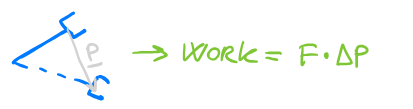
\includegraphics[width=0.3\linewidth]{images/statics_2}
	\label{fig:statics2}
\end{figure}

Sia anche
$$
\delta W_{g} = \bm{\tau}^T\delta\bm{q}
$$
il lavoro virtuale associato alle forze generalizzate ai giunti, ove $\delta\bm{q}$ è lo spostamento virtuale ai giunti.
Secondo il \textbf{principio dei lavori virtuali}, il manipolatore è in condizioni di equilibrio statico se e solo se i lavori virtuali delle forze generalizzate cartesiane e ai giunti sono uguali, qualunque sia la configurazione del robot:
$$
\delta W_g = \delta W_{TCP}
\iff
\bm{\tau}^T\delta \bm{q} = \bm{F}^T\delta\bm{p} \ \forall \bm{q}(t)
$$
Ora, visto che il nostro manipolatore è rappresentato da un sistema tempo-invariante (la configurazione dipenda da $\bm{q}(t)$, ma non esplicitamente dal tempo), possiamo dire che gli spostamenti virtuali coincidono con gli spostamenti elementari:
$$
\delta\bm{p}= d \bm{p}, \ \delta\bm{q} = d\bm{q}
$$

Richiamando $v=J(q)\dot{q}$ e che $v = dp/dt$, abbiamo:
$$
\bm{v} = \bm{J}(\bm{q})\bm{\dot{q}}
\iff
\frac{d\bm{p}}{\cancel{dt}} = \bm{J}(\bm{q}) \frac{d\bm{q}}{\cancel{dt}}
\iff
d\bm{p} = \bm{J}(\bm{q}) d\bm{q}
$$
dal principio dei lavori virtuali però abbiamo che  $\bm{F}^Td\bm{p} = \bm{\tau}^Td \bm{q}$, e quindi:
$$
d\bm{p} = \bm{J}(\bm{q}) d\bm{q}
\iff
\bm{\tau}d\bm{q} = \bm{F}^T\bm{J}(\bm{q})d\bm{q}
\iff
\bm{\tau}^T = \bm{F}^T\bm{J}
\iff
\bm{\tau} = \bm{J}^T\bm{F}
$$
Quindi, le forze ai giunti necessarie per bilanciare le forze sul TCP sono date da:
\begin{equation}\label{eq:static_equivalence}
\boxed{
\bm{\tau} = -\bm{J}^T(\bm{q})\bm{F}
}
\end{equation}
che è proprio la relazione statica cercata.




\section{Dualità cineto-statica}
In algebra lineare, 
$$
y = A^Tx \quad \text{è il problema duale di} \quad y = Ax
$$
quindi, dalla seguente osservazione:
\begin{figure}[H]
	\centering
	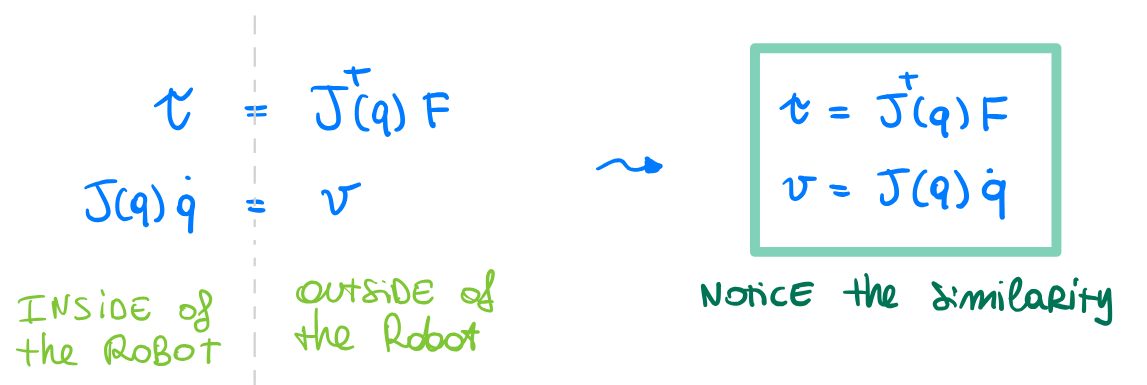
\includegraphics[width=0.7\linewidth]{images/statics_3}
	\label{fig:statics3}
\end{figure}
notiamo che possiamo vedere la relazione statica come il duale del problema della cinematica diretta delle velocità.

Prendiamo 
$$
\bm{F}^* \in \mathcal{N}(\bm{J}^T) \qquad s.t. \qquad \bm{J}^T\bm{F}^* = 0
$$
dalla relazione statica possiamo dire che $\bm{F}^*$ è un vettore di forze (applicate al TCP) che \underline{non} richiede alcuna compensazione dai motori: un esempio può essere visto in fig. \ref{fig:statics4}, dove abbiamo il braccio di un manipolatore a "penzoloni"; in questo caso abbiamo la forza di gravità che "tira" in giù, ma non sono necessarie alcune compensazioni da parte dei motori.
\begin{figure}[H]
	\centering
	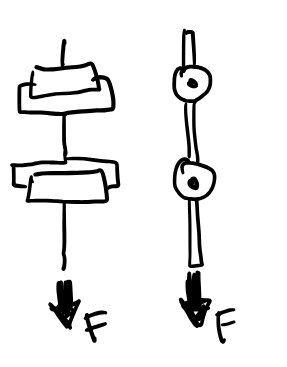
\includegraphics[width=0.2\linewidth]{images/statics_4}
	\caption{Esempio}
	\label{fig:statics4}
\end{figure}


Detto questo possiamo ora parlare più in dettaglio della relazione matematica che esiste fra $\bm{\tau}$ e $\bm{v}$. La dualità può essere caratterizzata dal range ed il kernel di $\bm{J}$ e $\bm{J}^T$:
\begin{itemize}
	\item $\mathcal{R}(\bm{J})$: velocità del TCP che possono essere raggiunte per una data posa
	\item $\mathcal{N}(\bm{J})$: velocità dei giunti che \underline{non} producono alcuna velocità nel TCP (per la data posa)
	\item $\mathcal{R}(\bm{J}^T)$: JFG ($\tau$) che riscono a bilanciare le forze generalizzate applicate al TCP ($F$), per la posa corrente
	\item $\mathcal{N}(\bm{J}^T)$: forze generalizzate applicate al TCP ($F$) che \underline{non} richiedono compensazione di JFG/coppie ($\tau$) (per la data posa)
\end{itemize}
Da algebra lineare, ricordiamo che:
$$
\mathcal{N}(\bm{J}) \equiv \mathcal{R}^\perp(\bm{J}^T)
\qquad
\mathcal{R}(\bm{J}) \equiv \mathcal{N}^\perp(\bm{J}^T)
$$
Da qui segue che, \textbf{quando il manipolatore è in configurazione singolare}:
\begin{itemize}
	\item Esistono velocità non nulle ai giunti $\dot{\bm{q}} \in \mathcal{N}(\bm{J})$ che producono velocità nulle della punta e \textbf{coppie generalizzate ai giunti} $\bm{\tau} \in \mathcal{N}(\bm{J}) = \mathcal{R}^\perp(\bm{J}^T)$ che non possono essere compensate da alcuna forza generalizzata sulla punta
	\item \textbf{Esistono forze generalizzate} $\bm{F} \in \mathcal{N}(\bm{J}^T)$ che non richiedono alcuna coppia ai giunti per essere bilanciata e velocità della punta operativa $\bm{v} = \mathcal{N}(\bm{J}^T) = \mathcal{R}^\perp(\bm{J})$ che non possono essere ottenute da velocità ai giunti
\end{itemize}




\section{Ellipsoidi di manipolabilità}

\subsection{Velocità}

Spesso, per sistemi lineari SISO, se ne studia il comportamento tramite la cosiddetta risposta all'impulso, che essenzialmente caratterizza il modo in cui il sistema risponde a un'unità di ingresso. Nel caso MIMO, invece (come per un manipolatore), il concetto analogo è quello di caratterizzare l'output in termini di un input con norma unitaria. Consideriamo quindi l'insieme di tutte le velocità dei giunti del robot $\bm{\dot{q}}$ tali che:
$$
\|\bm{\dot{q}}\|^2
= 
\dot{q}_1^2 + \dots + \dot{q}_n^2 
\ 
\leq 1
\iff
\bm{\dot{q}}^T\bm{\dot{q}} = 1
$$
usando $\bm{\dot{q}} = \bm{J}^\dagger \bm{v}$, si ottiene:
$$
\bm{\dot{q}}^T\bm{\dot{q}}
=
(\bm{J}^\dagger\bm{v})^T (\bm{J}^\dagger \bm{v})
=
\bm{v}^T (\bm{J}\bm{J}^T)^{-1}\bm{v}
$$
possiamo quindi definire il \textbf{velocity manipulability ellipsoid} come quei punti che soddisfano:
$$
E_v = \{\bm{v} \ : \ \bm{v}^T (\bm{J}\bm{J}^T)^{-1}\bm{v} = 1 \}
$$
notare che varia con il variare di $\bm{q}$. Da qui possiamo anche definire un'altro valore utile, chiamato \textbf{manipulability measure}:
$$
w(\bm{q}) = \sqrt{\det(\bm{J}\bm{J}^T)}
=
|\lambda_1\lambda_2 \cdots \lambda_n|
=
|\det(\bm{J})|
$$
che non è altro che il volume dell'ellissoide definito prima ($\lambda_i$ sono gli autovalori di $\bm{J}$).

Un'interessante osservazione può essere fatta per le \textbf{singolarità}: quando il manipolatore approccia una postura singolare abbiamo che $\lambda_i \to 0$ e quindi anche $w(\bm{q}) \to 0$ (non abbiamo manipolabilità!). Per questo motivo $w(\bm{q})$ è spesso usata come misura di "distanza" dalle configurazioni singolari.

\begin{figure}
	\centering
	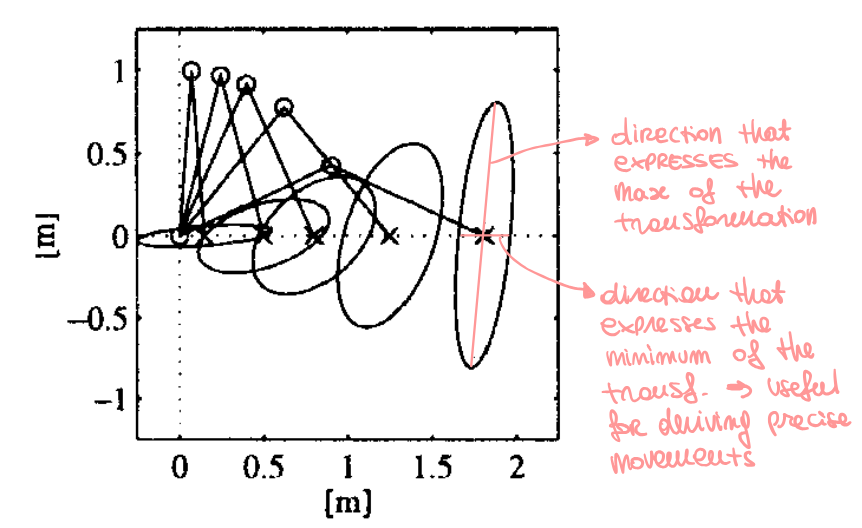
\includegraphics[width=0.6\linewidth]{images/statics_5}
	\caption{Ellissoidi di manipolabilità al variare della postura per un manipolatore con 2 giunti}
	\label{fig:statics5}
\end{figure}





\subsection{Forza}

Dalla dualità cineto-statica possiamo derivare un ellissoide di manipolabilità anche per le forze. Questa volta invece delle velocità dei giunti andiamo ad utilizzare le coppie generalizzate ai giunti:
$$
\bm{\tau}^T\bm{\tau} = 1
$$
allora, il \textbf{force manipulability ellipsoid} è definito come:
$$
E_F = \{\bm{F} \ : \ \bm{F}^T (\bm{J}\bm{J}^T)\bm{F} = 1 \}
$$
dove abbiamo utilizzato $\bm{\tau} = \bm{J}^T\bm{F}$.

\begin{figure}[H]
	\centering
	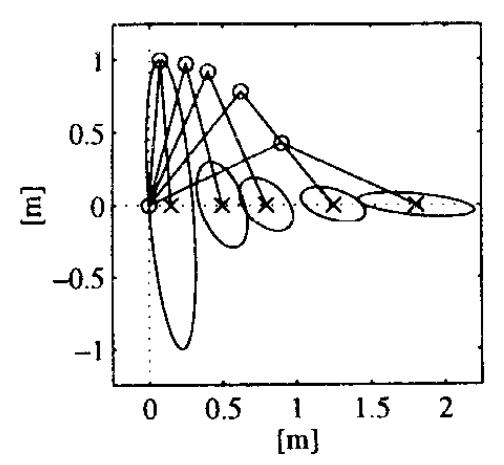
\includegraphics[width=0.3\linewidth]{images/statics_6}
	\caption{Stesso esempio di prima ma per la forza}
	\label{fig:statics6}
\end{figure}

Comparando la definizione di $E_F$ con quella di $E_v$ possiamo notare che in questo caso il contenuto fra le parentesi ($JJ^T$) non è invertito (mentre prima si): da qui consegue l'importante fatto che gli assi principali dell'ellissoide di manipolabilità della forza coincidono con quelli della velocità, ma con valori "inversi".\\
Da questo consegue un risultato anche intuitivo: \textbf{una direzione dove abbiamo una buona manipolabilità in velocità avrà cattiva manipolabilità di forza, e viceversa} $\rightarrow$ \textbf{veloce e debole \textit{oppure} lento e forte} (\textit{pensa al cambio di una bici/auto: in salita vado lento ma faccio tanta forza, in piano faccio meno forza ma vado più veloce}).

\begin{figure}
	\centering
	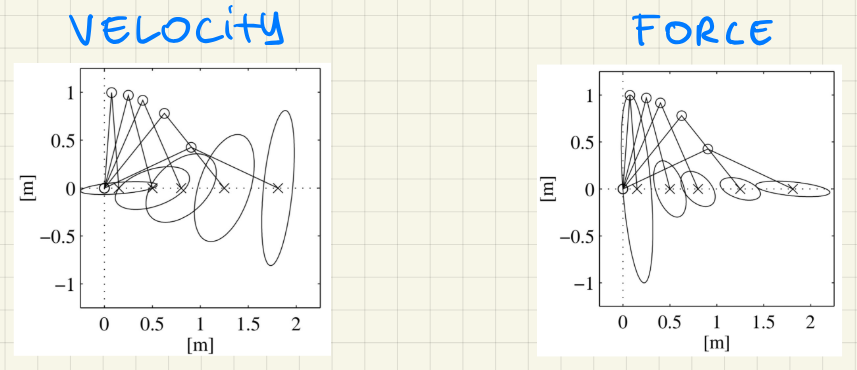
\includegraphics[width=0.6\linewidth]{images/statics_7}
	\caption{Comparazione: notare l'"inversione" fra i due}
	\label{fig:statics7}
\end{figure}



\chapter{Dinamica}

Passiamo ora a studiare la dinamica, ovvero le relazioni fra forze e movimenti.

Il modello dinamico del manipolatore può essere determinato seguendo due diversi approcci: equazioni di Lagrange oppure equazioni di Newton-Eulero. Dal punto di vista della derivazione le prime sono più semplici, mentre per quanto riguarda la computazione le seconde permettono algoritmi ricorsivi efficienti. Noi vedremo solo la definizione Lagrangiana.



\section{Lagrangiana ed equazioni di Eulero-Lagrange}

La \textbf{Lagrangiana} $\mathcal{L}$ di un sistema è data dalla differenza tra la sua energia cinetica totale $\mathcal{T}$ e la sua energia potenziale totale $\mathcal{U}$:
$$
\mathcal{\bm{L = T - U}}
$$
essa è funzione delle coordinate generalizzate usate per descrivere la posizione del sistema, nonché delle loro derivate rispetto al tempo. Nel caso di un manipolatore le variabili giunto qi possono essere assunte come coordinate generalizzate. 

Le equazioni di Eulero-Lagrange, che descrivono il comportamento dinamico del sistema, sono date da:
\begin{equation}\label{eq:euler-lagrange}
\frac{d}{dt}\left(\frac{\partial \mathcal{\bm{L}}}{\partial \dot{\bm{q}}_i}\right)
-
\frac{\partial \mathcal{\bm{L}}}{\partial \bm{q}_i}
=
\mathcal{\bm{F}}_i
\qquad
i = 1, \dots, n
\end{equation}
dove $\mathcal{\bm{F}}_i$ è la i-esima forza generalizzata, non conservativa (associata a $\bm{q}_i$).



\subsection{Energia cinetica}

L’energia cinetica totale di un manipolatore con $n$ giunti (e $n + 1$ bracci rigidi, ma il braccio di base $b_0$ non dà contributo, essendo fisso) è data dalla somma delle energie cinetiche $\mathcal{T}_{l_i}$ di ciascun braccio a cui vanno sommati i contributi $\mathcal{T}_{m_i}$ associati agli $n$ attuatori (motori) che muovono i giunti:
\begin{equation}\label{eq:kin_energy_sum}
\mathcal{T} = \sum_{i=1}^n \mathcal{T}_{l_i} + \mathcal{T}_{m_i}
\end{equation}


\subsubsection{Energia cinetica dei bracci}
Partiamo dalla seguente formulazione:
$$
\mathcal{T}_{l_i}
=
\frac{1}{2} m_{l_i} \bm{\dot{p}}_i^T \bm{\dot{p}}_i
+
\frac{1}{2} \bm{\omega}_i^T {}^b\bm{R}_i {}^i\bm{I}_{l_i} ({}^b\bm{R}_i)^T \bm{\omega}_i
$$
dove le velocità (traslazionali e rotazionali) sono indicate rispetto al centro di massa del braccio, e $\bm{I}_{l_i}$ rappresenta il tensore di inerzia del braccio $i$.


\begin{proof2}
Dalla definizione fisica:
$$
\mathcal{T}_{l_i}
=
\frac{1}{2} \int_{V_{l_i}} \underbrace{\bm{\dot{p}}_i^T \bm{\dot{p}}_i}_{\textit{velocity}^2} \underbrace{\rho dV}_{mass}
$$
usando la formula della derivata di un vettore
$$
\dot{p}_i = \dot{p}_{\ell_i} + \omega_i \times r_i = \dot{p}_{\ell_i} + S(\omega)r_i
$$
sostituendo alla precedente otteniamo (skippando i calcoli, vedi slide):
$$
\mathcal{T}_{l_i}
=
\frac{1}{2} m_{l_i} \bm{\dot{p}}_i^T \bm{\dot{p}}_i
+
\frac{1}{2} \bm{\omega}_i^T \bm{I}_{l_i} \bm{\omega}_i
$$

Ora dobbiamo però notare che il tensore di inerzia di un corpo rigido, rispetto al suo centro di massa, è costante solo se espresso in un sistema di riferimento locale solidale con il corpo ed avente origine con il centro di massa stesso.

Nel caso sopra mostrato abbiamo espresso $\bm{I}_{l_i}$ nel base-frame, e quindi non costante. Possiamo però utilizzare il tensore relativo al link-frame, trasformandolo le approriate matrici: 
$$
I_{l_i} = {}^bR_i {}^iI_{l_i} ({}^bR_i)^T
$$
dove ${}^bR_i$ è la matrice di rotazione del link-frame w.r.t base-frame.\\ Effettuando questa sostituzione abbiamo la tesi.
\end{proof2}



Ora, richiamando (\ref{eq:geom_jacob_2}), possiamo seguire lo stesso concetto e scrivere:
\begin{gather*}
\dot{\bm{p}}_{l_i}
=
\bm{J}^{(l_i)}_{p,1}\dot{\bm{q}}_1
+
\bm{J}^{(l_i)}_{p,2}\dot{\bm{q}}_2
+ \cdots +
\bm{J}^{(l_i)}_{p,i}\dot{\bm{q}}_i
=
\bm{J}^{(l_i)}_{p}\dot{\bm{q}}_i
\\
\bm{\omega}_{l_i}
=
\bm{J}^{(l_i)}_{o,1}\dot{\bm{q}}_1
+
\bm{J}^{(l_i)}_{o,2}\dot{\bm{q}}_2
+ \cdots +
\bm{J}^{(l_i)}_{o,i}\dot{\bm{q}}_i
=
\bm{J}^{(l_i)}_{o}\dot{\bm{q}}_i
\end{gather*}
dove $\bm{J}^{(l_i)}_{u,j}$ è la $j$-esima colonna di $\bm{J}^{(l_i)}_{u}$.

Queste due nuove matrici $\bm{J}^{(l_i)}_{o}, \bm{J}^{(l_i)}_{o}$ seguono un concetto analogo a quello delle colonne dello Jacobiano geometrico, però invece di far riferimento all'intero manipolatore, riguardano solo il link $i$:
\begin{itemize}
	\item Se il giunto è prismatico:
	\begin{align*}
		\bm{J}^{(l_i)}_{p,j} &= \bm{k}_{j-1} \\
		\bm{J}^{(l_i)}_{o,j} &= \bm{0}
	\end{align*}
	\item Se il giunto è rotoidale:
	\begin{align*}
		\bm{J}^{(l_i)}_{p,j} &= \bm{k}_{j-1} \times (\bm{p}_{l_j} - \bm{p}_{j-1} ) \\
		\bm{J}^{(l_i)}_{o,j} &= \bm{k}_{j-1}
	\end{align*}
\end{itemize}
per entrambi le formule valgono $\forall j = 1,\dots,i$.

Quindi, usando quest'ultime formulazioni possiamo riscrivere la forma iniziale come:
$$
\mathcal{T}_{l_i}
=
\frac{1}{2} m_{l_i} \left(\bm{\dot{q}}^T \bm{J}_p^{(l_i)T}\right) \left(\bm{J}_p^{(l_i)} \bm{\dot{q}}\right)
+
\frac{1}{2} 
\left(\bm{\dot{q}}^T \bm{J}_o^{(l_i)T}\right)
\left( {}^b\bm{R}_i {}^i\bm{I}_{l_i} ({}^b\bm{R}_i)^T \right)
\left(\bm{J}_o^{(l_i)} \bm{\dot{q}}\right)
$$

Alla fin fine, però questa formulona non è altro che 
$$
\frac{1}{2} \bm{\dot{q}}^T \textit{roba}(\bm{q}) \bm{\dot{q}}
=
\frac{1}{2}m\bm{v}^2
$$
ovvero l'energia cinetica.




\subsubsection{Energia cinetica dei motori}

Un ragionamento analogo può essere fatto per i motori. Inanzitutto supponiamo che il motore $i$-esimo che attua il giunto $i$ sia localizzato sul braccio $i-1$, come mostrato in fig. \ref{fig:dynamics1}.
\begin{figure}[H]
	\centering
	\includegraphics[width=0.3\linewidth]{images/dynamics_1}
	\caption{Posizionamento motore}
	\label{fig:dynamics1}
\end{figure}
Inoltre, per semplicità supponiamo che il contributo delle trasmissioni (gears) possa essere incluso nel motore stesso e che non ci siano movimenti indotti (i.e. il giunto i non muove altri giunti).

Quindi, analogamente ai bracci:
$$
\mathcal{T}_{m_i}
=
\frac{1}{2} m_{m_i} \bm{\dot{p}}_i^T \bm{\dot{p}}_i
+
\frac{1}{2} \bm{\omega}_i^T {}^b\bm{R}_i {}^i\bm{I}_{m_i} ({}^b\bm{R}_i)^T \bm{\omega}_i
$$
dove nuovamente le velocità sono relative al centro di massa e il tensore di inerzia è relativo al base frame. Facendo le solite sostituzioni:
$$
\mathcal{T}_{m_i}
=
\frac{1}{2} m_{m_i} \left(\bm{\dot{q}}^T \bm{J}_p^{(m_i)T}\right) \left(\bm{J}_p^{(m_i)} \bm{\dot{q}}\right)
+
\frac{1}{2} 
\left(\bm{\dot{q}}^T \bm{J}_o^{(m_i)T}\right)
\left( {}^b\bm{R}_{m_i} {}^{m_i}\bm{I}_{m_i} ({}^b\bm{R}_{m_i})^T \right)
\left(\bm{J}_o^{(m_i)} \bm{\dot{q}}\right)
$$
dove l'unica differenza è che qui il tensore di inerzia è relativo ad un sistema di riferimento locale, solidale con il rotore (avente l’asse z diretto lungo il suo asse di rotazione), e ${}^b\bm{R}_{m_i}$ è la relativa matrice di rotazione.

Per la definizione di $\bm{J}_u^{(m_i)}$ abbiamo una differenza solo per la parte di orientamento (oltre alla ovvia sostituizione $\bm{p}_{l_j} \rightarrow \bm{p}_{m_j}$), che diventa:
\begin{align*}
	\begin{cases}
		\bm{J}^{(m_i)}_{o,j} = \bm{J}^{(l_i)}_{o,j} & \quad j=1,\dots,i-1 \\
		\bm{J}^{(m_i)}_{o,j} = k_{ri}\bm{z}_{mi} & \quad j=i
	\end{cases}
\end{align*}
per entrambi i tipi di giunti.


\vspace*{5pt}
\subsubsection{Energia cinetica totale}
Ritornando all'energia cinetica totale, possiamo inserire i nostri risultati dentro (\ref{eq:kin_energy_sum}) ed ottenere:
\begin{equation}\label{eq:kin_energy}
\boxed{
\mathcal{T}
= 
\frac{1}{2}
\sum_{i=1}^n
\sum_{j=1}^n
b_{ij}(\bm{q}) \dot{\bm{q}}_i \dot{\bm{q}}_j
=
\frac{1}{2} \dot{\bm{q}}^T \bm{B}(\bm{q}) \dot{\bm{q}}
}
\end{equation}
dove $\bm{B}(\bm{q})$ è la matrice d’inerzia (data dalla somma dei vari termini visti prima), simmetrica, definita positiva e configuration-dependent. Infine notiamo che $\mathcal{T}$ è funzione sia delle posizioni sia delle velocità dei giunti.





\subsection{Energia potenziale}
In maniera analoga all'energia cinetica, definiamo:
\begin{equation}\label{eq:pot_energy_sum}
	\mathcal{U} = \sum_{i=1}^n \mathcal{U}_{l_i} + \mathcal{U}_{m_i}
\end{equation}
L’ipotesi che il manipolatore sia costituito da bracci rigidi implica l’assenza di elementi nella sua struttura che possano immagazzinare energia potenziale, di conseguenza essa è dovuta solo alla presenza della forza di gravità:
\begin{gather*}
	\begin{aligned}
		\mathcal{U}_{l_i} &= -m_{l_i}\bm{g}_0^T \bm{p}_{l_i} \\
		\mathcal{U}_{m_i} &= -m_{m_i}\bm{g}_0^T \bm{p}_{m_i}
	\end{aligned} \\
\Downarrow \\
\boxed{
\mathcal{U} = - \sum_{i=1}^n m_{l_i}\bm{g}_0^T \bm{p}_{l_i} + m_{m_i}\bm{g}_0^T \bm{p}_{m_i}
}
\end{gather*}
dove $\bm{g}_0^T$ è il vettore di accelerazione gravitazionale nel base-frame (\textit{e.g. $\bm{g}_0^T = (0,0,-g)$ se l'asse $z$ è diretto verso l'alto}).





\section{Equazioni dinamiche del manipolatore}
Essendo ormai note le espressioni di $\mathcal{T}$ e $\mathcal{U}$, è possibile calcolare la funzione Lagrangiana $\mathcal{L}$ come:
$$
\mathcal{L}(\bm{q}, \bm{\dot{q}})
=
\mathcal{T}(\bm{q}, \bm{\dot{q}})
-
\mathcal{U}(\bm{q})
$$
e quindi ricavare le equazioni dinamiche del manipolatore dalle equazioni di Eulero-Lagrange (\ref{eq:euler-lagrange}). Eseguendo le derivate richieste si otteiene:

\begin{equation}\label{eq:robot_dynamics}
\boxed{\sum_{j=1}^n \bm{B}_{ij}(\bm{q}) \ddot{q}_j
+
\sum_{j=1}^n \sum_{k=1}^n h_{ijk} (\bm{q}) \dot{q}_k \dot{q}_j 
+
g_i(\bm{q})
=
\mathcal{F}_i
\qquad
i = 1, \dots, n
}
\end{equation}
dove
$$
h_{ijk}
=
\frac{\partial B_{ij}}{\partial q_k}
-
\frac{1}{2} \frac{\partial B_{jk}}{\partial q_i}
$$
e il termine $g_i(q)$ dovuto alla gravità risulta pari a:
$$
g_i(\bm{q})
=
\frac{\partial \mathcal{U}}{\partial q_i}
=
-\sum_{j=1}^n m_{l_j}\bm{g}_0^T \bm{J}^{(l_j)}_{p_i}(\bm{q}) + m_{m_j}\bm{g}_0^T  \bm{J}^{(m_j)}_{p_i}(\bm{q})
$$

La stessa formula può essere riscritta in forma compatta come
\begin{equation}\label{eq:robot_dynamics_short}
\boxed{
	\bm{B}(\bm{q})\bm{\ddot{q}} + \bm{n}(\bm{q}, \bm{\dot{q}}) = \mathcal{\bm{F}}
}
\end{equation}
oppure
\begin{equation}\label{eq:robot_dynamics_short2}
\boxed{
	\bm{B}(\bm{q})\bm{\ddot{q}} + \bm{C}(\bm{q}, \bm{\dot{q}})\bm{q} + \bm{g}(\bm{q})= \mathcal{\bm{F}}
}
\end{equation}
in modo che sia una \textit{comoda} EDO di 2° ordine. I due nuovi termini sono definiti come:
%$$
%\sum_{j=1}^n \bm{B}_{ij}(\bm{q}) \ddot{q}_j
%+
%\underbrace{
%\sum_{j=1}^n \sum_{k=1}^n h_{ijk} (\bm{q}) \dot{q}_k \dot{q}_j 
%}_{\triangleq \ \bm{C}(\bm{q}, \bm{\dot{q}})\bm{q}}
%+
%g_i(\bm{q})
%=
%\mathcal{F}_i
%$$
\begin{figure}[H]
	\centering
	\includegraphics[width=0.5\linewidth]{images/dynamics_2}
	\label{fig:dynamics2}
\end{figure}


%\begin{equation}\label{eq:dynamic_n_def}
%\boxed{
%\bm{n}(\bm{q}, \bm{\dot{q}}) 
%\triangleq
%\bm{\dot{B}}(\bm{q})\bm{\dot{q}}
%-
%\frac{1}{2}\left( \frac{\partial}{\partial \bm{q}} (\bm{\dot{q}}^T \bm{B}(\bm{q})\dot{\bm{q}} ) \right)^T 
%+
%\left( \frac{\partial \mathcal{U}(\bm{q})}{\partial \bm{q}} \right)
%}
%\end{equation}



\subsection{Interpretazione fisica dei termini}

\begin{itemize}
	\item Termini "di \textbf{accelerazione}": $\sum_{j=1}^n \bm{B}_{ij}(\bm{q}) \ddot{q}_j$
	\begin{itemize}
		\item $\bm{B}_{ii}(\bm{q})$ rappresenta il momento di inerzia equivalente sull’asse del giunto $i$-esimo nella configurazione $\bm{q}$, quando tutti gli altri giunti sono fermi
		\item $\bm{B}_{ii}(\bm{q})$ con $i\neq j$, tiene conto degli effetti delle accelerazioni del giunto $j$ sul giunto $i$
	\end{itemize}
	
	\item Termini "quadratici in \textbf{velocità}": $\sum_{j=1}^n \sum_{k=1}^n h_{ijk} (\bm{q}) \dot{q}_k \dot{q}_j$
	\begin{itemize}
		\item $h_{ijj}(\bm{q}) \dot{q}_j^2$ tiene conto degli effetti sul giunto $i$ della \textbf{forza centrifuga} dovuta al moto del giunto $j$
		\item $h_{ijk}(\bm{q}) \dot{q}_j \dot{q}_k$ tiene conto degli \textbf{effetti di Coriolis} indotti sul giunto $i$ dalle velocità dei giunti $j$ e $k$
	\end{itemize}
	
	\item Termini "dipendenti dalla configurazione": $g_i(\bm{q})$
	\begin{itemize}
		\item Rrappresenta il momento generato sul giunto $i$ dalla forza di gravità, nella configurazione $\bm{q}$
	\end{itemize}
\end{itemize}




\subsection{Forze non conservative}
Ci manca solo da valorizzare il vettore delle forze generalizzate $\bm{\mathcal{F}}$. In generale possiamo dire che:
$$
\bm{\mathcal{F}}
=
\underbrace{\bm{\tau}}_{\substack{\text{coppie attive} \\ \text{di comando}}}
-
\underbrace{\bm{F}_v\dot{\bm{q}}}_{\substack{\text{coppie di} \\ \text{attrito viscoso}}}
-
\underbrace{\bm{F}_s \text{sgn}(\dot{\bm{q}}) }_{\substack{\text{coppie di} \\ \text{attrito statico}}}
-
\underbrace{\bm{J}^T(\bm{q}) \bm{h}}_{\substack{\text{coppie generate per bilanciare} \\ \text{forze di contatto esterne}}}
$$
dove $\bm{h}$ è il vettore delle forze generalizzate applicate \textit{dalla} punta operativa \textit{sull}’ambiente esterno.
Sostiuendo a (\ref{eq:robot_dynamics_short2}) e riordinando i termini otteniamo:
\begin{equation}\label{eq:robot_dynamics_short_complete}
	\boxed{
		\bm{B}(\bm{q})\bm{\ddot{q}} + \bm{C}(\bm{q}, \bm{\dot{q}})\bm{q}		+
		\bm{F}_v\dot{\bm{q}} 
		+
		\bm{F}_s \text{sgn}(\dot{\bm{q}})
		+
		\bm{g}(\bm{q})
		= 
		\bm{\tau}
		-
		\bm{J}^T(\bm{q}) \bm{h}
	}
\end{equation}
nuovamente abbiamo una forma di una EDO di 2° ordine: $\alpha\ddot{q} + \beta \dot{q} + g(q) = \mathcal{F}$
\chapter{Traiettorie}
\chapter{Controllo}

Il problema del controllo del moto di un manipolatore consiste nella \textbf{determinazione} dell’andamento temporale delle coppie generalizzate (\textbf{generalized torque)}, che gli attuatori devono applicare ai giunti \textbf{affinché venga eseguito il compito assegnato}, rispettando specifiche sul transitorio e sul comportamento in regime permanente.

Lo schema di controllo può essere sviluppato:
\begin{enumerate}
	\item Nello \textbf{spazio dei giunti}
	\item Nello \textbf{spazio operazionale}
\end{enumerate}

tenendo conto che la descrizione del compito è solitamente elaborata nello spazio operazionale, mentre le azioni di controllo esercitate dagli attuatori sono definite nello spazio dei giunti.\\

\subsubsection{Joint space control}
\begin{figure}[!ht]
	\centering
	\includegraphics[width=0.7\linewidth]{images/joint_control_1}
	\caption{Schema generale di \textit{joint space control}}
	\label{fig:jointcontrol1}
\end{figure}

L’azione di controllo fa sì che $q(t)$ insegua il vettore $q_d(t)$ della traiettoria desiderata ai giunti, ricavato dalla cinematica inversa (che è comodamente disaccoppiata dal controllo).

\textbf{Svantaggio}: Non si ha nè un feedback, nè un controllo diretto sulla variabile dello spazio operazionale $\mathbf{p}$ $\implies$ dobbiamo avere una cinematica inversa perfetta (ma tolleranze di costruzione, elasticità ai giunti, giochi nei motoriduttori potrebbero causare imprecisioni).\\



\subsubsection{Operational space control}
\begin{figure}[ht!]
	\centering
	\includegraphics[width=0.7\linewidth]{images/operational_control_1}
	\caption{Schema generale di \textit{operational space control}}
	\label{fig:operationalcontrol1}
\end{figure}

Qui cerchiamo di fare inseguire un vettore $\mathbf{p}_d$ definito nello spazio operazionale. Con questa tecnica introduciamo una \textbf{complessità maggiore}, visto che la cinematica inversa è ora inclusa nel controllore. Il \textbf{vantaggio} però è quello di poter operare direttamente nello spazio operazionale.\\
Anche se in primo luogo potrebbe non sembrare un vantaggio (la “misura” di $\mathbf{p}$ è spesso ricavata indirettamente da misure ai giunti per mezzo della cinematica diretta $\implies$ sembra lo stesso svantaggio di imprecisione della cinematica inversa che c'era nel controllo sui giunti): questo controllo è però utile (ad esempio) come base per il controllo dell’interazione con l’ambiente.\\

\subsubsection{Cosa vedremo}
Vedremo che la presenza di \textbf{motoriduttori} con elevato rapporto di trasformazione tende a \textbf{linearizzare la dinamica} del manipolatore e quindi a disaccoppiare i giunti, grazie alla riduzione degli effetti non lineari $\implies$ si giustifica in tal caso l’adozione di una strategia di \textbf{controllo decentralizzato}, a giunti indipendenti. 

Questo però introduce uno svantaggio: i motoriduttori introducono possibili fenomeni di elasticità, gioco ed attriti non lineari, talora più "fastidiosi" degli effetti di accoppiamento fra i giunti. L’utilizzo di \textbf{motori ad azione diretta} elimina questi problemi ma mantiene rilevanti gli effetti non lineari e di accoppiamento fra i giunti, che non possono essere trascurati o considerati come disturbi $\implies$ diventa opportuno in tal caso utilizzare una strategia di \textbf{controllo centralizzato}, che tenga conto della dinamica non lineare del manipolatore. \textbf{Svantaggio}: la legge di controllo è necessariamente non lineare e computazionalmente pesante.





\section{Attuatori elettrici}
Prima di introdurre i sistemi di controllo, iniziamo parlando di come poter modellare gli attuatori elettrici che andremmo ad utilizzare.

Gli attuatori maggiormente impiegati sono motori DC o brushless. Fortunatamente dal punto di vista matematico, un motore DC e un brushless dotato degli appositi sensori, possono essere modellati allo stesso modo.
A seconda delle caratteristiche del regolatore inserito, il comportamento dell’attuatore può essere assimilato:
\begin{itemize}
	\item Ad un generatore di velocità controllata (\textbf{velocity controlled})
	\item Ad un generatore di coppia controllata (\textbf{torque controlled})
\end{itemize}

In fig. \ref{fig:electricactuator1} possiamo vedere il modello del motore che utilizzeremo. Notazione usata:

\begin{itemize}
	\item $\omega_m$ e $\theta_m$ sono la velocità e la posizione angolare dell’albero
	motore
	\item $V_a$ e $I_a$ sono la tensione e la corrente del circuito di armatura
	\item $\tau_m$ è la coppia motrice, mentre $\tau_r$ è la coppia dovuta al carico
\end{itemize}

\begin{figure}[th!]
	\centering
	\includegraphics[width=0.7\linewidth]{images/electric_actuator_1}
	\caption{Modello del motorore comandato in armatura}
	\label{fig:electricactuator1}
\end{figure}


\subsection{Derivazione modello}

Partendo dal circuito illustrato in fig. \ref{fig:electricactuatorcircuit} (il quale modella un motore DC), possiamo derivare il circuito mostrato in fig. \ref{fig:electricactuator1}.

\begin{figure}[th!]
	\centering
	\includegraphics[width=0.7\linewidth]{electric_actuator_circuit.jpg}
	\caption{Modello circuitale del motore}
	\label{fig:electricactuatorcircuit}
\end{figure}

Il bilancio elettrico dell'armatura è definito da:
\begin{align}\label{eq:armature_balance}
L\frac{dI_a}{dt} + RI_a = V_a - V_b
\quad
\xRightarrow{\mathcal {L}}
\quad
\begin{aligned}
V_a &= (R_a + sL_a)I_a + V_g\\
V_g &= K_{\omega} \omega_m
\end{aligned}
\end{align}
Dove $V_g$ è la \textbf{\textit{back-emf}}, ovvero quella tensione generata dalla dal movimento delle coils del motore nel campo magnetico (e questa tensione è proporzionale alla velocità del conduttore nel campo, ovvero a $\omega_m = \dot{\theta}_m$). Questa tensione, tenderà ad opporsi al flusso di corrente nel conduttore.

Il bilancio meccanico è invece definito da:
\begin{align}
\tau_m &= (s\Gamma_m + \beta_m)\omega_m + \tau_r \\
\tau_m &= K_i\Gamma_a
\end{align}
Dove $\Gamma_m$ e $\beta_m$ sono rispettivamente il momento d'inerzia e il coefficiente di attrito viscoso dell'albero motore. Queste formule derivano da:
\begin{enumerate}
	\item Ricordando da fisica 1: $F = ma \leftrightsquigarrow \tau = I\alpha$ dove $I$, $\alpha$ sono il momento di inerzia e l'accellerazione angolare
	\item Allora, facendo riferimento al motore: $\tau = I\alpha \ \rightsquigarrow \ \tau_m = \Gamma_m\dot{\omega}_m$
	\item Ora "aggiungiamo" l'attrito viscoso (che come ricordiamo è proporzionale alla velocità): $\tau_m - \beta_m\omega_m = \Gamma_m\dot{\omega}_m$
	\item Infine, passando a Laplace: $\tau_m = \beta_m\omega_m + \Gamma_m s\omega_m \implies \tau_m = (s\Gamma_m + \beta_m)\omega_m \quad \square$ 
\end{enumerate}


\subsection{Amplificatore di potenza}
Visto che solitamente $V_a$ ha valori elevati, si tende ad utilizzare un \textbf{amplificatore di potenza} per poter comandare il motore con una tensione $V_c \ll V_a$: il nuovo circuito è illustrato in fig. \ref{fig:electricactuator2}. 

$G_v$ è il guadagno di tensione, mentre $T_v$ è una costante di tempo trascurabile (poiché nell’ordine di 10-100 kHz), di conseguenza il blocco dell’amplificatore di potenza può essere assimilato al solo guadagno $G_v$.


\begin{figure}[th!]
	\centering
	\includegraphics[width=0.7\linewidth]{images/electric_actuator_2}
	\caption{Modello motore con amplificatore di potenza}
	\label{fig:electricactuator2}
\end{figure}




\subsection{Velocity generator}

Possiamo ora completare il circuito aggiungendo una retroazione sulla corrente $I_a$ e un compensatore che utilizzi tale feedback. \\
Prima di vedere l'effetto della retroazione, però, iniziamo dal caso più semplice, dove $K_i = 0$: in questa modalità riusciamo ad impostare a piacimento la velocità del motore, giocando sulla tensione di controllo $V_c^{'}$.

\begin{figure}[H]
	\centering
	\includegraphics[width=0.7\linewidth]{images/electric_actuator_4}
	\caption{Circuito motore in modalità velocity generator}
	\label{fig:electricactuator4}
\end{figure}

Per dimostrare quando affermato, analizziamo lo steady-state del circuito in fig. \ref{fig:electricactuator4}. Ricordandoci che il coefficiente di atttrito viscoso meccanico $\beta_m$ è trascurabile rispetto al coefficiente di attrito viscoso elettrico (\textit{mi son dimenticato come si ricava ma avevo chiesto al prof e aveva senso}):
$$
\beta_m \ll \frac{K_\omega K_t}{R_a}
$$
e supponendo $C_i(s) = 1$, $\tau_r = 0$ (per semplicità di calcolo), otteniamo:
$$
\omega_m \approx \frac{G_v}{K_\omega}V^{'}_c
$$

Ovvero, in questo caso, possiamo impostare la velocità angolare a piacere (per la derivazione del valore di steady-state vedi appendice \ref{appendix:torque_controlled_steady_state_derivation}).





\subsection{Torque generator}\label{section:torque_generator}

Passiamo ora al caso in cui $K_i \neq 0$: circuito in fig. \ref{fig:electricactuator3}. In questa modalià, vedremo invece che è possibile controllare a piacere la coppia (al posto della velocità come nel caso precedente).

\begin{figure}[!th]
	\centering
	\includegraphics[width=0.7\linewidth]{images/electric_actuator_3}
	\caption{Circuito motore in modalità torque generator}
	\label{fig:electricactuator3}
\end{figure}

Adesso, come accennato, il motore si comporta come un \textit{torque-controlled generator}. Questo perchè, con $K_i \neq 0$, se si sceglie $K_i \gg R_a$ otteniamo il seguente steady-state (la derivazione segue lo stesso ragionamento usato per il caso velocity-controlled):
$$
\tau_m \approx \frac{K_t}{K_i}(V^{'}_c - \frac{K_\omega}{G_v}\omega_m)
\approx
\frac{K_t}{K_i}V^{'}_c
$$
(supponendo $G_v \gg 1 \implies \frac{K_\omega}{G_v} \to 0$). Questo significa che possiamo impostare il torque del motore giocando sul voltaggio di controllo $V^{'}_c$.





\subsection{Torque generator \textit{vs.} Velocity generator}


Quando ci conviene utilizzare uno invece che l'altro?
In seguito vedremo che in tutte le applicazioni in cui è necessario ottenere un’elevata reiezione di coppie di disturbo, come nel caso del \textbf{controllo decentralizzato a giunti indipendenti}, è opportuno NON inserire l’anello di controllo in corrente ed utilizzare i motori come \textbf{generatori di velocità}.

Al contrario, in caso di strategie di \textbf{controllo centralizzate}, è consigliabile introdurre l’anello di retroazione in corrente ed utilizzare i motori come \textbf{generatori di coppie} (opportuni accorgimenti vengono adottati in entrambi i casi per limitare la corrente ed evitare danni ai dispositivi).

E' possibile vedere questa differenza calcolando le relazioni input/output fra $\omega_m$ e $V^{'}_c$, $\tau_r$. Da queste equazioni si può vedere che senza feedback di corrente (i.e. velocity-controlled generator) si ha una reiezione migliore della coppia di disturbo $\tau_r$: i coefficienti legati a $\tau_r$ in questo caso sono molto minori del caso torque-controlled ($\implies$ riduciamo di più gli effetti dei disturbi).

Semplificando:
\begin{align}
\omega_m^{\text{velocity}} &= \alpha_{\text{velocity}} V^{'}_c + \lambda_{\text{velocity}}\tau_r \\
\omega_m^{\text{torque}} &= \alpha_{\text{torque}} V^{'}_c + \lambda_{\text{torque}}\tau_r
\end{align}

se il primo è per il caso velocity-controlled, mentre il secondo per il caso torque-controlled abbiamo che $\lambda_{\text{velocity}} \ll \lambda_{\text{torque}}$.







\section{Trasmissions {\small \textit{aka}} motoriduttori}
Vediamo ora in dettaglio gli effetti che i motoriduttori utilizzati nel motore hanno sul sistema.

\begin{figure}[th!]
	\centering
	\includegraphics[width=0.5\linewidth]{images/trasmission_1}
	\caption{Motoriduttore}
	\label{fig:trasmission1}
\end{figure}


In generale, se indichiamo con $k_r$ il rapporto di trasformazione (\textit{gear-ratio}) di un motoriduttore ideale, abbiamo che:
$$
\theta_m = k_r\theta
$$
ove $\theta_m$ è la posizione angolare dell’albero motore e $\theta$ è la posizione angolare sul secondario (giunto). $k_r$ è invece definito come il rapporto tra i raggi dei due \textit{gears}:
$$
k_r = \frac{r}{r_m} = \frac{\theta_m}{\theta} = \frac{\omega_m}{\omega}
$$
Considerando attriti viscosi e coppie, possiamo scrivere le equazioni di equilibrio:
$$
\begin{array}{l c r}
	{\tau_{_\mathrm{m}}=\Gamma_{_\mathrm{m}}\dot{\omega}_{\mathrm{m}}+\beta_{_\mathrm{m}}\omega_{\mathrm{m}}+\mathrm{fr}_{_{\mathrm{m}}}}\\ {\mathrm{fr}=\Gamma\dot{\omega}+\beta_{_\mathrm{g}}\omega+\tau_{\mathrm{d}}}
\end{array}
$$
(La forza $f$ scambiata tra i due ingranaggi genera una coppia di reazione $fr_m$ per il moto all'asse del motore ed una coppia motrice $fr$ per il moto di rotazione del carico).\\
Dopo alcuni passaggi si ottiene:
$$
\tau_m = \left( \Gamma_m + \frac{\Gamma}{k_r^2} \right) \dot{\omega}_n
+
\left( \beta_m + \frac{\beta_g}{k_r^2} \right)\omega_m
+
\frac{\tau_d}{k_r}
$$
Notiamo che \textbf{qualunque coppia applicata sul secondario è riportata sul primario ridotta del fattore $k_r$ (e viceversa).} \\
Poiché $\mathbf{k_r}$ \textbf{è elevato}, l’effetto di coppie di \textbf{disturbo} agenti sul secondario risulta \textbf{fortemente ridotto} sul primario. Se tali coppie dipendono non-linearmente da $\theta$, allora la presenza di un alto fattore di riduzione tende a \textbf{linearizzare il sistema}.

Nel caso vettoriale (molteplici giunti), possiamo riscrivere alcune utili relazioni:
\begin{align}
	\mathbf{q}_m = \mathbf{K}_r\mathbf{q} \label{eq:trasmission_reduction}\\\
	\boldsymbol{\tau}_m = \mathbf{K}_r^{-1} \boldsymbol{\tau} \label{eq:trasmission_reduction_torque}
\end{align}
Dove quest'ultima deriva (intuitivamente) dal fatto che con l'aumentare del \textit{gear-ratio} si diminiusce la velocità angolare ma si aumenta il torque (e viceversa).

\section[Controllo decentralizzato a giunti indipendenti]{Controllo decentralizzato a giunti indipendenti \\ {\small \textit{Decentralized Joint Space Control}}}

Nel controllo decentralizzato a giunti indipendenti \textbf{ogni} singolo \textbf{giunto} attuato è considerato come un \textbf{sottosistema SISO disaccoppiato e indipendente}, descritto da un modello dinamico approssimato. Gli \textbf{effetti di accoppiamento} non-lineari presenti nella dinamica propria del robot sono \textbf{considerati come disturbi}.

Lo schema di controllo complessivo è formato da $n$ controllori (uno per ogni giunto), basati su reti di compensazione classiche, ciascuno agente in modo indipendente dagli altri.\\
Ricordiamo che il nostro obiettivo è quello di far eseguire una sequenza $\mathbf{q}(t)$ in modo che $\mathbf{q}(t) \to \mathbf{q}_d(t)$.\\	


\begin{figure}[th!]
	\centering
	\includegraphics[width=0.7\linewidth]{images/decentralized_joint_space_control_1}
	\caption{Schema generale del controllo a giunti indipendenti}
	\label{fig:decentralizedjointspacecontrol1}
\end{figure}


Come accennato in precedenza, in questo caso andremo a controllare gli attuatori in velocità (questo esce in "automatico" dalle equazioni: vedi sezione \ref{section:single_joint_control}).

\textit{Ora qua Rizzo ha detto roba che non ho capito. Lo stesso concetto si deriva comunque seguendo i prossimi discorsi. Per vedere quello che ha detto Rizzo vedi appendice \ref{appendix:decentralized_joint_control_velocity_controlled}}

Richiamando i capitoli precedenti, ricordiamo che il modello dinamico del manipolatore (in assenza di forze scambiate con l’ambiente esterno) è espresso da:
\boldmath
\begin{equation}\label{eq:dynamic_no_ext_forces}
B(q)\ddot{q} + C(q, \dot{q})\dot{q} + F_v\dot{q} + g(q) = \tau = K_r \tau_m
\end{equation}
\unboldmath

L'ultima uguaglianza deriva dall'utilizzo dei motoriduttori (vedi (\ref{eq:trasmission_reduction_torque})).

Per elaborare uno schema di controllo decentralizzato ai giunti è opportuno riportare le equazioni dinamiche a monte del motoriduttore (sul primario, i.e. lato motore):
\boldmath
$$
K_r^{-1}B(q)K_r^{-1}\ddot{q}_m + K_r^{-1}C(q, \dot{q})K_r^{-1}\dot{q}_m + K_r^{-1}F_vK_r^{-1}\dot{q} + K_r^{-1}g(q) = \tau_m
$$
\unboldmath

(Questa equazione è ottenuta semplicemente applicando (\ref{eq:trasmission_reduction}) e (\ref{eq:trasmission_reduction_torque}) a (\ref{eq:dynamic_no_ext_forces})).

È possibile notare che $\mathbf{B}(q)$ può essere decomposto in $\mathbf{B}(q) = \bar{\mathbf{B}} + \Delta\mathbf{B}(q)$, ove $\bar{\mathbf{B}}$ è una matrice diagonale costante e $\Delta\mathbf{B}(q)$ è una matrice configuration-dependent. Possiamo quindi riscrivere l'ultima equazione come:
\boldmath
\begin{gather*}
(\bar{B} + \Delta B(q)) K_r^{-1} \ddot{q} + C(q, \dot{q})K_r^{-1}\dot{q} + F_vK_r^{-1}\dot{q} + g(q) = K_r \tau_m \\
\Downarrow \\
K_r^{-1}\bar{B}K_r^{-1}\ddot{q}_m + d + K_r^{-1}F_vK_r^{-1}\dot{q}_m  = \tau_m
\end{gather*}
dove possiamo considerare gli effetti degli altri giunti su quello corrente come \textbf{disturbi}:
\begin{equation}\label{eq:dynamic_disturbances}
	d \triangleq K_r^{-1}\Delta B(q)K_r^{-1}\ddot{q}_m + K_r^{-1}C(q, \dot{q})K_r^{-1}\dot{q}_m + K_r^{-1}g(q)
\end{equation}

Inoltre, visto che questi termini sono moltiplicati per $\mathbf{K}_r^{-1}$, \textbf{più alto è il gear-ratio e meno questi termini influenzeranno il nostro sistema} ($d \downarrow$ quando $K_r \uparrow$), portandoci così ad un sistema sempre più lineare e disaccoppiato (ovviamente c'è un limite, visto che gear-ratio altissimi non produrrebbero praticamente alcune velocità).

Riassumendo:
\begin{equation}\label{eq:dynamic_with_disturbances}
K_r^{-1}\bar{B}K_r^{-1}\ddot{q}_m + F_m\dot{q}_m + d = \tau_m
\end{equation}
dove $F_m \triangleq K_r^{-1}F_vK_r^{-1}$. 
\unboldmath



\begin{figure}[t]
	\centering
	\includegraphics[width=0.7\linewidth]{images/decentralized_joint_space_control_2}
	\caption{Circuito relativo a (\ref{eq:dynamic_with_disturbances})}
	\label{fig:decentralizedjointspacecontrol2}
\end{figure}

Detto questo, per la parte lineare possiamo ora far riferimento alla nota teoria del controllo LTI per sistemi SISO.






\subsection{Controllo del singolo giunto}\label{section:single_joint_control}

Partendo da (\ref{eq:dynamic_with_disturbances}) possiamo estrarre la relazione per un singolo giunto:
\begin{equation}\label{eq:single_joint_dynamic}
\Gamma \ddot{q}_m + \beta \dot{q}_m + d = \tau_m
\end{equation}
dove $\Gamma$ e $\beta$ sono rispettivamente il momento di inerzia totale equivalente ed il coefficiente di attrito viscoso totale equivalente, definiti come segue 
\footnote{notando che ${\mathbf{K}_r}_i^{-1} \alpha {\mathbf{K}_r}_i^{-1} = (1/{\mathbf{K}_r}_i^2) \alpha $}:
$$
\Gamma = \frac{1}{{\mathbf{K}_r}_i^2} \mathbf{\bar{B}}_{ii} 
\quad , \quad
\beta = \frac{1}{{\mathbf{K}_r}_i^2} {\mathbf{F}_m}_i, 
$$

Passando a Laplace (con condizioni iniziali nulle) otteniamo:
\begin{equation}\label{eq:single_joint_dynamic_laplace}
(s\Gamma + \beta) \omega_m(s) = \tau_m(s) - d(s)
\end{equation}
considerando $\omega_n(s)$ come uscita, otteniamo il circuito di fig. \ref{fig:decentralizedjointspacecontrol3}: notare che questo \textbf{\underline{coincide} col modello del motore in modalità velocity-generator} (fig. \ref{fig:electricactuator4}) con $C_i(s) = 1$ $\implies$ \textbf{usiamo attuatore in modalità velocity-controlled}.

\begin{figure}[th!]
	\centering
	\includegraphics[width=0.7\linewidth]{images/decentralized_joint_space_control_3}
	\caption{Schema a blocchi del singolo giunto}
	\label{fig:decentralizedjointspacecontrol3}
\end{figure}


Cerchiamo ora di semplificare un po' questo modello. Possiamo iniziare supponendo $L_a$ trascurabile, dato che le perdite ad essa associate sono solitamente molto piccole.
Dall'equazione di equilibrio elettrico (\ref{eq:armature_balance}) possiamo quindi rimuovere $L_a$, e ottenere:
\begin{equation}\label{eq:simplified_armature_electrical_balance}
V_a - R_aI_a = K_\omega \omega_m
\end{equation}
Allora, ricordando che $I_a = \tau_m K_t^{-1}$ e sostituendo $\tau_m$ con l'espressione (\ref{eq:single_joint_dynamic_laplace}) otteniamo 
$$
V_a - R_a K_t^{-1} \tau_m = K_\omega \omega_m
\implies
V_a - R_a K_t^{-1} ((s\Gamma + \beta)\omega_m + d)
= K_\omega \omega_m
$$



Riorganizzando i termini, e ignorando il termine relativo a $\beta$ (visto che è trascurabile rispetto a $\omega_m$), otteniamo:
$$
\left( \frac{R_a \Gamma}{K_t K_\omega}s + 1 \right) \omega_m =
\frac{1}{K_\omega}V_a - \frac{R_a}{K_tK_\omega}d
$$

Da qui possiamo identificare 2 funzioni di trasferimento (a seconda di cosa consideriamo ingresso):
\begin{align}
G_\omega(s) &\triangleq \frac{\omega_m(s)}{V_a(s)} = \frac{1}{K_\omega(1 + sT)} \label{eq:tf_omega} \\
G_d(s) &\triangleq \frac{\omega_m(s)}{d(s)} = -\frac{T}{\Gamma(1 + sT)} = -K_dG_\omega(s)
\end{align}
dove:
$$
T = \frac{R_a \Gamma}{K_t K_\omega} 
\quad , \quad
K_d = \frac{R_a}{K_t}
$$

Da queste equazioni possiamo quindi passare allo schema a blocchi di fig. \ref{fig:decentralizedjointspacecontrol4}.

\begin{figure}[H]
	\centering
	\includegraphics[width=0.6\linewidth]{images/decentralized_joint_space_control_4}
	\caption{Schema a blocchi semplificato}
	\label{fig:decentralizedjointspacecontrol4}
\end{figure}




\vspace*{25pt}
\begin{mdframed}[leftmargin=15pt, rightmargin=15pt, leftline=false, rightline=false]
\subsubsection{Comparazione con le slide di Rizzo}
\textit{Nelle slide è presente il seguente circuito. Anche se a prima vista potrebbe sembrare diverso è in realtà identico a quello di figura \ref{fig:decentralizedjointspacecontrol4}.}

{
	\centering
	\includegraphics[width=0.6\linewidth]{images/decentralized_joint_space_control_5}
	\label{fig:decentralizedjointspacecontrol5}
	\par
}

\textit{Ricordando la differente notazione: $I \equiv \Gamma$, $k_v \equiv K_\omega$, possiamo unire i 3 blocchi in uno unico. Partiamo dal forward path:}
$$
F(s) = \frac{k_t}{R_a sI}
$$
\textit{Poi, incorporando il feedback, otteniamo}
$$
\frac{F(s)}{1 + F(s)k_v} = 
\frac{ \frac{k_t}{R_a sI} }{1 +  \frac{k_v k_t}{R_a sI} } = \frac{1}{k_v(1 + sT)}
$$

\textit{Ovvero la stessa forma di quanto mostrato in fig. \ref{fig:decentralizedjointspacecontrol4}.}
\end{mdframed}




\vspace{25pt}
\subsection{Struttura del controllo}

In fig. \ref{fig:decentralizedjointspacecontrol6} possiamo vedere lo schema di controllo generale, con retroazione su posizione, velocità e accelerazione (nota: per semplicità $G_v$ è stato incluso nell'anello di controllo più interno).

In generale, il controllore viene progettato modo che si abbia un guadagno elevato nel blocco a monte del punto di ingresso del disturbo (per ottenere un elevato fattore di attenuazione) e in modo che ci sia un’azione integrale, affinché gli effetti della coppia di gravità vengano cancellati in regime permanente.

\begin{figure}[H]
	\centering
	\includegraphics[width=0.9\linewidth]{images/decentralized_joint_space_control_6}
	\caption{Schema generale del controllo}
	\label{fig:decentralizedjointspacecontrol6}
\end{figure}


Queste richieste portano alla scelta di un \textbf{controllore PI (proporzionale-integrale)} della forma:
\begin{equation}\label{eq:pi_controller}
C(s) = K_p \frac{1+sT_p}{s}
\end{equation}





\vspace*{10pt}
\subsubsection{Retroazione sulla posizione}
Possiamo partire dal caso più semplice, ovvero introducento un controllo con solo la retroazione $k_{TP}$ su $\theta_m$. Poniamo $C_v(s) = C_A(s) = 1$ e $k_{TV} = k_{TA} = 0$, mentre mettiamo $C_p(s)$ nella forma (\ref{eq:pi_controller}).

\begin{figure}[ht!]
	\centering
	\includegraphics[width=0.7\linewidth]{images/position_feedback}
	\caption{Solo position feedback}
	\label{fig:positionfeedback}
\end{figure}

\begin{figure}
	\centering
	\includegraphics[width=0.7\linewidth]{images/position_feedback_control}
	\caption{Circuito di fig. \ref{fig:positionfeedback} con blocco motore accorpato ($q_{r,m}\equiv\theta_r$, $q_m \equiv \theta_m$)}
	\label{fig:positionfeedbackcontrol}
\end{figure}



La funzione di trasferimento del ramo diretto risulta (richiamando (\ref{eq:pi_controller}) e (\ref{eq:tf_omega})):
$$
G(s) = 
\underbrace{K_p \frac{1+sT_p}{s}}_{C_p(s)=(\ref{eq:pi_controller})}
\underbrace{ \frac{1}{K_\omega(1 + sT)} }_{G_\omega(s) =(\ref{eq:tf_omega})}
\frac{1}{s}
= \frac{K_p(1+sT_p)}{s^2K_\omega(1+sT)}
$$
da cui si ricava la funzione di trasferimento ad anello chiuso:
$$
W(s) = \frac{K_p(1+sT_p)}{s^2K_\omega(1+sT) + K_P K_{TP} (1+sT_P)}
$$

Da qui è possibile analizzarne la stabilità, ad esempio tramite il luogo delle radici (vedi fig. \ref{fig:rootlocus1}).

\begin{figure}[ht!]
	\centering
	\includegraphics[width=0.7\linewidth]{images/root_locus_1}
	\caption{Root locus per $W(s)$ con solo retroazione sulla posizione}
	\label{fig:rootlocus1}
\end{figure}


I parametri $K_P$ e $T_P$ devono essere scelti in modo da:
\begin{itemize}
	\item Garantire l’asintotica stabilità del sistema in catena chiusa
	\item Evitare oscillazioni significative nella sua risposta
	\item Garantire un elevato fattore di attenuazione del disturbo 
\end{itemize}


Per calcolare meglio i requirements è possibile esprimere $W(s)$ in funzione di $\omega_n$ e $\zeta$:
$$
W(s) = \frac{\frac{1}{K_{TP}}(1+sT_P)}{\left( 1 + \frac{2\zeta}{\omega_n} + \frac{s^2}{\omega_n^2} \right) (1+\tau s) }
$$

Come possiamo vedere anche dal root locus:
\begin{itemize}
	\item Deve essere $T_P > T$ affinché si abbia asintotica stabilità
	\item Se $T_P \gg T$ si velocizza la risposta del sistema (diventano dominanti i poli complessi coniugati). Inoltre per elevati valori del guadagno $K_P$ la pulsazione del polo reale di $W(s)$ tende a quella dello zero ($\tau \approx T_P$) e quindi il sistema risulta rappresentato in prima approssimazione dalla sola dinamica del II° ordine associata ai poli complessi coniugati
	\item La parte reale dei poli dominanti non può comunque essere inferiore a $-1/(2T)$
\end{itemize}

Applicando le regole dell'algebra dei blocchi, è possibile anche ricavare la funzione di trasferimento fra il disturbo $D$ e l’uscita $\theta_m$ del sistema:
$$
\frac{\Theta_m(s)}{D(s)} = 
-K_d\frac{
\frac{s}{K_pK_{TP}(1+sT_p)}
}
{1 + \frac{s^2K_\omega(1+sT)}{K_PK_{TP}(1+sT_P)}}
$$
Da questa t.f. è possibile vedere che \textbf{il fattore di attenuazione del disturbo vale} $\mathbf{K_PK_{TP}}$. Valori troppo elevati di $K_P$ possono però portare ad avere oscillazioni inaccettabili sull’uscita (lo smorzamento $\zeta$ risulta troppo piccolo).\\
Il tempo necessario per avere un’attenuazione significativa del disturbo è approssimabile come $T_R = max\{T_P, \frac{1}{\zeta \omega_n}\}$








\vspace{35pt}
\subsubsection{Retroazione di posizione e velocità}

Per questo secondo caso consideriamo il seguente setup (qua $C_A(s)=1$, $k_{TA}=0$), rappresentato in fig. \ref{fig:decentralizedjointspacecontrol7}:
$$
C_P(s) = K_P \qquad C_V(s)=K_V\frac{1+sT_V}{s}
$$
Ovvero un'azione solo proporzionale per la posizione, mentre un'azione PI per la velocità. \\
La costante di tempo $T_V$ può essere scelta in modo da cancellare il polo meccanico del giunto attuato: 
$$
T_V = T
$$

\begin{figure}[ht!]
	\centering
	\includegraphics[width=0.7\linewidth]{images/decentralized_joint_space_control_7}
	\caption{Circuito con retroazione su posizione e velocità}
	\label{fig:decentralizedjointspacecontrol7}
\end{figure}

Come per il caso precedente, possiamo analizzare la stabilità del sistema tramite il root-locus della funzione di trasferimento in ciclo chiuso $W(s)$:
$$
W(s)=\frac{K_P K_V}{K_\omega s^2 + K_V K_{TV} s + K_{TP} K_P K_V}
$$
e gli effetti dei disturbi con la funzione di trasferimento $\Theta_m(s)/D(s)$ (saltando la definizione della forma esplicita): in questo caso il \textbf{fattore di attenuazione del disturbo} è dato dal prodotto $\mathbf{K_P K_{TV} K_V}$, ormai completamente definito, avendo imposto $K_P$ e $K_V$ per imporre i poli desiderati.

Aumentando il guadagno del feedback di posizione $K_P$, è possibile confinare i poli dell'anello chiuso in una regione del piano complesso con grandi valori assoluti della parte reale. Poi, la posizione effettiva può essere stabilita mediante una scelta adeguata di $K_V$.

\begin{figure}[!ht]
	\centering
	\includegraphics[width=0.5\linewidth]{images/root_locus_2}
	\caption{Root-locus con retroazione di velocità e posizione}
	\label{fig:rootlocus2}
\end{figure}







\vspace{35pt}
\subsubsection{Retroazione di posizione, velocità ed accelerazione}

Per concludere vediamo il controllo con tutti e 3 i feedback:
$$
C_P(s) = K_P \qquad C_V(s)=K_V \qquad C_A(s)=K_A\frac{1+sT_A}{s}
$$

Avendo a disposizione un parametro libero in più, sarebbe
possibile in questo caso:
\begin{itemize}
	\item Assegnare la dinamica desiderata al sistema ad anello chiuso
	\item Imporre il fattore di attenuazione del disturbo
\end{itemize}


\begin{figure}[ht!]
	\centering
	\includegraphics[width=0.5\linewidth]{images/root_locus_3}
	\caption{Root-locus con retroazione di accelerazione, velocità e posizione}
	\label{fig:rootlocus3}
\end{figure}

\textbf{Problema}:
La misura dell’\textbf{accelerazione però non è solitamente disponibile}. Per implementare uno schema di controllo comprendente la retroazione dell’accelerazione risulterebbe necessario ricavarla indirettamente dalle misure disponibili.

Avendo a disposizione la misura diretta della velocità, è possibile \textbf{stimare l’accelerazione} per mezzo di un filtro del primo ordine (vedi fig. \ref{fig:accelerationestimate}), purché avente banda sufficientemente ampia. Scegliendo questa larghezza di banda sufficientemente ampia, gli effetti dovuti ai ritardi di misurazione non sono un problema, e quindi è possibile prendere l'uscita del filtro di accelerazione come quantità per il feedback. Problemi possono comunque incorrere a causa del rumore presente sul segnale di accelerazione così ottenuto.

\begin{figure}[H]
	\centering
	\includegraphics[width=0.4\linewidth]{images/acceleration_estimate}
	\caption{Filtro del I° ordine per la stima dell'accelerazione}
	\label{fig:accelerationestimate}
\end{figure}







\subsection{Attuatori saturanti}
In un’applicazione reale, il comportamento del sistema può allontanarsi da quello del suo modello teorico a causa di dinamiche “parassite” o non lineari, non incluse nella descrizione considerata, con evidenti conseguenze sulle prestazioni del controllo. Una di queste è ad esempio la presenza di attuatori saturanti.

Quest'ultima però può essere modellata semplicemente aggiugendo sul ramo diretto dell’anello di controllo un blocco che rappresenta la seguente relazione:
$$
\begin{cases}
	y_{max} & , \ u(t) > u_{max} \\
	ku(t) & , \ u_{min} \leq u(t) \leq u_{max} \\
	y_{min} & , \ u(t) < u_{min}
\end{cases}
$$


\begin{figure}[H]
	\centering
	\includegraphics[width=0.4\linewidth]{images/saturation}
	\label{fig:saturation}
\end{figure}


L’inserimento di blocchi di \textbf{saturazione} è solitamente legato a \textbf{necessità di sicurezza e di salvaguardia} del sistema.

Quando le grandezze coinvolte (correnti, tensioni) raggiungono il valore massimo consentito ed entra in azione il blocco di saturazione, l’inseguimento della traiettoria non è più realizzato con le caratteristiche e l’accuratezza prevista. In caso di movimenti PTP non è inusuale che vengano raggiunte situazioni di saturazione: in tal caso infatti è solitamente prioritario raggiungere il più rapidamente possibile la configurazione finale desiderata, anziché rispettare la traiettoria prefissata in ogni istante.







\subsection{Feedforward compensation}
Quando è richiesto l’inseguimento di traiettorie con elevati valori di velocità e di accelerazione, è possibile ridurre l’errore di inseguimento utilizzando i valori del riferimento in velocità (ed in accelerazione) per calcolare termini di compensazione in avanti (feedforward compensation), da sommare all’azione del controllore posto sul ramo diretto.

Si noti che, in generale, calcolare derivate non è possibile (perchè dovremmo "predire il futuro"). In questo caso però essendo la traiettoria nota a priori, non ci sono problemi.

\begin{figure}[H]
	\centering
	\includegraphics[width=0.7\linewidth]{images/feedforward_compensation}
	\caption{Schema a blocchi del controllo con feedback di posizione e feedforward compensation decentralizzato}
	\label{fig:feedforwardcompensation}
\end{figure}





\subsection{Computed torque	feedworward control}\label{section:computed_torque}
È possibile aggiungere un altro blocco di feedforward.
Richiamando (\ref{eq:dynamic_with_disturbances}):
\boldmath
$$
K_r^{-1}\bar{B}K_r^{-1}\ddot{q}_m + F_m\dot{q}_m + d = \tau_m
$$
\unboldmath
se vogliamo reiettare perfettamente il disturbo $d$ potremmo provare a calcolarci in anticipo il valore di $d$, per poi sommarlo nel lato destro dell'equazione.
\boldmath
$$
K_r^{-1}\bar{B}K_r^{-1}\ddot{q}_m + F_m\dot{q}_m + \cancel{d} = \tau_m + \cancel{d}
$$
\unboldmath
Ponendo $q\equiv q_d$ ci basta usare (\ref{eq:dynamic_disturbances}) per calcolarci $d$ (calcolo fatto offline).
 
\begin{figure}[H]
	\centering
	\includegraphics[width=0.7\linewidth]{images/computed_torque}
	\caption{Circuit with computed torque feedworward control}
	\label{fig:computedtorque}
\end{figure}



\section[Controllo centralizzato ai giunti]{Controllo centralizzato ai giunti \\ \small \textit{Centralized Joint Space Control}}

In alcuni casi il \textbf{controllo decentralizzato} a giunti indipendenti \textbf{può risultare inadeguato}. Questo accade, ad esempio, quando:
\begin{itemize}
	\item sono \textbf{richieste velocità operative elevate} $\implies$ le coppie di disturbo strutturato dipendenti dalla velocità (di Coriolis, centrifughe) influiscono pesantemente sul comportamento dei giunti
	\item i \textbf{motori sono ad azione diretta} $\implies$ a causa dell’assenza dei motoriduttori ($\mathbf{K}_r = \mathbf{I}$) non si beneficia di alcuna riduzione degli effetti non lineari e di accoppiamento fra i giunti
\end{itemize}
 
In tali casi gli effetti delle coppie di disturbo $\mathbf{d}$ possono determinare errori troppo elevati di inseguimento della traiettoria.
 
Poiché in questi casi non è possibile ridurre sufficientemente gli effetti indotti dalle coppie di disturbo $\mathbf{d}$, diventa conveniente cercare di eliminare direttamente tali coppie, ricorrendo ad una \textbf{strategia di controllo contenente termini non lineari di compensazione}.\\
Si parla di \textbf{controllo centralizzato} perché la coppia applicata a ciascun giunto risulta funzione anche delle variabili di posizione e velocità degli altri giunti, a differenza di quanto accade nel controllo a giunti indipendenti.
 
Negli schemi di controllo centralizzato il manipolatore è considerato come un \textbf{unico sistema MIMO}, con n ingressi (le coppie applicate ai giunti) e n uscite (le posizioni dei giunti) che interagiscono fra loro secondo relazioni non lineari. La \textbf{legge di controllo} centralizzato dovrà tenere conto del modello dinamico del manipolatore ed essere \textbf{non-lineare} (visto che il modello è non lineare).
 
 
 
 
 


\vspace*{20pt}
\subsubsection{Ora usiamo attuatori torque-controlled}
Come accennato all'inizio in questo caso userremo motori in modalità generatori di coppia. Intuitivamente queseto segue dal fatto che gli attuatori dovranno fornire coppie tali da compensare “esattamente” (o quanto meglio possibile) i disturbi strutturati: da questo si consegue che è opportuno utilizzare i motori come generatori di coppia anziché di velocità.

Richiamando la forma semplificata del bilancio elettrico di armatura (\ref{eq:simplified_armature_electrical_balance}), possiamo scrivere:
$$
I_a = R_a^{-1}(V_a - K_\omega \omega_m) = R_a^{-1}(G_vV_c - K_\omega \omega_m)
$$
Dove l'ultima ugualianza deriva dall'amplificatore di potenza: $V_a = G_v V_c$.
Di conseguenza, ricordando (sempre al modello del motore: vedi fig. \ref{fig:electricactuator1}), che $\tau_m = K_t I_a$, possiamo scrivere:
$$
\tau = K_r \tau_m = K_r K_t I_a = K_r K_t R_a^{-1}(G_vV_c - K_\omega \omega_m)
$$
che si può notare essere uguale a (\ref{eq:torque_command}).

Visto che però vogliamo avere un motore torque-controlled è necessario inserire la corrente in retroazione. 
%Visto che $\omega_m = K_r\omega$ e $K_r \gg 1$, abbiamo che $K_\omega\omega_m \to 0$
Per magimagia (forse vedi sezione \ref{section:torque_generator}) diciamo che il termine con $K_\omega$ diventa trascurabile e quindi:
$$
I_a = R_a^{-1}(G_vV_c - \cancel{K_\omega\omega_m}) = G_i V_c
$$
Di conseguenza
\boldmath
$$
\tau = K_r K_t G_i V_c = u
$$
\unboldmath
ove $\mathbf{u}$ è il vettore di comandi disponibili per il controllo.







\vspace*{20pt}
\subsection{Controllo a dinamica inversa}\label{section:joint_space_inverse_dyn_contr}

Il principale approccio di controllo centralizzato è detto a \textbf{dinamica inversa}, ed è basato sull’idea di ottenere una \textbf{linearizzazione della dinamica del sistema per mezzo di una retroazione non lineare} degli stati tale da condurre ad un sistema lineare e disaccoppiato rispetto ad un nuovo vettore di accelerazioni di comando da progettare. \\
Detto in altre parole, applichiamo la tecnica nota come \textbf{feedback linearization}.

Prima di cominciare, per comodità definiamo il modello della dinamica come:
\boldmath
\begin{equation}\label{eq:simplified_notation_dynamic}
B(q)\ddot{q} + n(q, \dot{q}) = \tau = u
\end{equation}
dove:
$$
n(q, \dot{q}) \triangleq C(q, \dot{q})\dot{q} + F_v\dot{q} + g(q)
$$
\unboldmath

Supponendo di poter calcolare esattamente $\mathbf{B(q)}$ e $\mathbf{n(q, \dot{q})}$, definiamo il nostro comando di controllo come
\boldmath
$$
u = B(q)y + n(q, \dot{q})
$$
questo perchè, così facendo, riusciamo ad ottenere una \textbf{linearizzazione esatta del sistema}:
\begin{gather*}
B(q)\ddot{q} + \cancel{n(q, \dot{q})} = \tau = u = B(q)y + \cancel{n(q, \dot{q})} \\
\Updownarrow \\
\cancel{B(q)}\ddot{q} = \cancel{B(q)}y \\
\Updownarrow \\
\ddot{q} = y
\end{gather*}
Il sistema risultante è costituito da n doppi integratori: la i-esima componente $y_i$ del nuovo comando influenza solo il comportamento della i-esima coordinata giunto $q_i$, che risulta indipendente dal moto degli altri giunti.


\begin{figure}[H]
	\centering
	\includegraphics[width=0.8\linewidth]{images/centralized_control_1}
	\caption{Feedback linearization}
	\label{fig:centralizedcontrol1}
\end{figure}

La scelta più semplice per il nuovo comando $\mathbf{y}$ è data da una legge di \textbf{controllo di tipo PD}:
$$
y = -K_P q - K_D \dot{q} + r
$$

che quindi, sostituendo a $\ddot{q} = y$, otteniamo il seguente sistema di equazioni del secondo ordine:
\begin{equation}\label{eq:2nd_order_dyn_feedback_lin}
\ddot{q} + K_D \dot{q} + K_P q = r
\end{equation}
asintoticamente stabile se le matrici $K_P$ e $K_D$ sono definite positive.
Scegliendo in particolare $K_P$ e $K_D$ diagonali, il sistema rimane disaccoppiato e ad ogni variabile giunto viene assegnata la dinamica corrispondente ai guadagni imposti con:
\unboldmath
$$
\mathbf{K_P} = diag\{\omega_{n1}^2, \ \dots, \ \omega_{nn}^2\}
\quad
\mathbf{K_D} = diag\{2\zeta\omega_{n1}, \ \dots, \ 2\zeta\omega_{nn}^2\}
$$

\boldmath
Il vettore di riferimento $r$ è definito a partire dalla traiettoria desiderata, \textbf{pianificata ai giunti}, come:
$$
r \triangleq \ddot{q}_d + K_D \dot{q}_d + K_P q_d 
$$
Possiamo ora analizzare la dinamica dell'errore di inseguimento, sostituendo la definizione di $r$ a (\ref{eq:2nd_order_dyn_feedback_lin}):
$$
(\ddot{q}_d - \ddot{q}) + K_D(\dot{q}_d - \dot{q}) + K_P(q_d - q) = 0
\implies
\ddot{e} + K_D\dot{e} + K_Pe = 0
$$
se $e(0) = 0$ e $\dot{e}(0) = 0$, l'errore converge a 0 con velocità e caratteristiche determinate da $K_P$ e $K_D$.
\unboldmath

Il sistema risultante è mostrato in fig. \ref{fig:centralizedcontrol2}, dove notiamo due anelli: quello più interno è l'anello di linearizzazione, mentre quello esterno è il controllo (ora lineare) del nostro sistema.

\begin{figure}
	\centering
	\includegraphics[width=0.7\linewidth]{images/centralized_control_2}
	\caption{Schema a blocchi del controllo a dinamica inversa nello spazio dei giunti}
	\label{fig:centralizedcontrol2}
\end{figure}


\vspace*{20pt}
\subsubsection{Problemi}
L’ipotesi di linearizzazione esatta presuppone la capacità di calcolare \textit{online} le matrici $\mathbf{B(q)}$ e $\mathbf{n(q, \dot{q})}$ in modo esatto. Nella pratica però questo non è sempre possibile.
Per compensare a questi errori è necessario utilizzare altre tecniche, ad esempio algoritmi di controllo robusto.

Supponiamo di avere solo delle approssimazioni delle matrici, che chiameremo $\mathbf{\hat{B}(q)}$ e $\mathbf{\hat{n}(q, \dot{q})}$:
\boldmath
\begin{gather*}
B(q)\ddot{q} + n(q, \dot{q}) = \hat{B}(q)y + \hat{n}(q, \dot{q}) \\
\Updownarrow \\
\ddot{q} = B^{-1}\hat{B}y + B^{-1}(\hat{n} - n) \\
\Updownarrow \\
\ddot{q} = y + (B^{-1}\hat{B} - I)y + B^{-1}(\hat{n} - n) \\
\Updownarrow \\
\ddot{q} = y - \eta(q, \dot{q}, y) \\
\Downarrow \\
\ddot{e} + K_D\dot{e} + K_Pe = \eta(q, \dot{q}, y)
\end{gather*}
dove
$$
\eta(q, \dot{q}, y) \triangleq (I - B^{-1}\hat{B})y - B^{-1}(\hat{n} - n)
$$

Il sistema ottenuto non è più lineare e disaccoppiato.

Per fortuna, \textbf{nella pratica}, il metodo della dinamica inversa \textbf{risulta abbastanza robusto} anche nel caso di linearizzazione approssimata, per cui viene usato sia senza ulteriori modifiche, sia con l’aggiunta di un termine robustificante.\\

\vspace*{5pt}
\subsubsection{Vari schemi visti come dinamica inversa}
Tra gli schemi a dinamica inversa con linearizzazione approssimata, che non prevedono l’inserimento di termini robustificanti, possiamo includere:
\begin{itemize}
	\item \textbf{Controllo a giunti indipendenti}: questo approccio precedentemente analizzato può essere considerato come un caso particolare di controllo a dinamica inversa con linearizzazione approssimata, ottenuto ponendo:
	$$
	\hat{B}(q) = \bar{B} \quad , \quad \hat{n}(q, \dot{q}) = 0
	$$
	\item \textbf{Metodo della coppia calcolata} (o controllo a dinamica inversa in feedforward): visto in sezione \ref{section:computed_torque}
	\item \textbf{Controllo PD con compensazione della gravità}, che vediamo nella prossima sezione; questo controllo può essere visto come dinamica inversa ponendo:
	$$
	\hat{B}(q) = I \quad , \quad \hat{n}(q, \dot{q}) = g(q)
	$$
\end{itemize}
\unboldmath








\vspace*{7pt}
\subsection{Controllo PD con compensazione della gravità}

Nel caso in cui si voglia assegnare al manipolatore una \textbf{postura di equilibrio costante} (anziché una traiettoria completa), è possibile realizzare un controllore tale da garantire la stabilità asintotica globale di tale postura.

\boldmath
Facendo riferimento a (\ref{eq:simplified_notation_dynamic}): $B(q)\ddot{q} + n(q, \dot{q}) = u$, definiamo il controllo come:
$$
u \triangleq g(q) + K_P(q_d - q) - K_D\dot{q}
$$
Così facendo, sostituendo $u$ a (\ref{eq:simplified_notation_dynamic}), otteniamo:
\begin{equation}\label{eq:pd_gravity_comp_dyn}
B(q)\ddot{q} + C(q, \dot{q})\dot{q} + F_v\dot{q} + \cancel{g(q)} = \cancel{g(q)} + K_P(q_d - q) - K_D\dot{q}
\end{equation}

Ovvero si riescono a cancellare gli effetti della gravità.

\begin{figure}[H]
	\centering
	\includegraphics[width=0.6\linewidth]{images/centralized_control_pd_gravity_comp}
	\caption{Controllo PD con compensazione della gravità}
	\label{fig:centralizedcontrolpdgravitycomp}
\end{figure}
(notare che nel circuito non è presente $\dot{q}_d$: questo poichè essendo $q_d$ costante la sua derivata è nulla)

Analizzando il sistema risultante da (\ref{eq:pd_gravity_comp_dyn}), possiamo vedere che l'unico punto di equilibrio è dato da $q \equiv q_d$:
\unboldmath
\begin{align*}
x \ \text{punto di equilibro} 
&\iff 
\dot{x} = \begin{pmatrix}\dot{q} \\ \ddot{q}\end{pmatrix} = 0
\stepcounter{equation}\tag{\theequation}\label{eq:pd_grav_comp_equil} \\
\textit{\footnotesize{sostituendo a (\ref{eq:pd_gravity_comp_dyn})}}
&\iff 
B(q)\cancelto{0}{\ddot{q}} + C(q, \dot{q})\cancelto{0}{\dot{q}} + F_v\cancelto{0}{\dot{q}} = K_P(q_d - q) - K_D\cancelto{0}{\dot{q}} \\
&\iff
0 = K_P(q_d - q) \\
\textit{\footnotesize{essendo $K_P > 0$}}
&\iff
q = q_d
\end{align*}

Ovvero proprio quello che volevamo: stabilità in una postura costante $\mathbf{q}_d$.

Per fare un esempio, immagina il robot in figura \ref{fig:centralizedcontrolpdgravitycompexample}: il motori dovranno applicare delle coppie (i quali valori dipendono dal valore di $\mathbf{u}$ mostrato prima) per far rimanere il braccio in questa posizione statica.

\begin{figure}[H]
	\centering
	\includegraphics[width=0.5\linewidth]{images/centralized_control_pd_gravity_comp_example}
	\caption{Esempio di compensazione gravità}
	\label{fig:centralizedcontrolpdgravitycompexample}
\end{figure}




\vspace*{20pt}
\subsubsection{Dimostrazione stabilità}
\boldmath
Per dimostrare le caratteristiche di stabilità del punto di equilibrio corrispondente alla postura desiderata, è possibile applicare il \textbf{metodo diretto di Lyapunov}. Definiamo $e \triangleq q_d - q$ e consideriamo come funzione di Lyapunov:
$$
V(\dot{q}, e) = \frac{1}{2}\dot{q}^TB(q)\dot{q} + \frac{1}{2}e^TK_Pe > 0    \qquad \forall q,e\neq0
$$
Dove possiamo interpretare il primo termine come l’energia cinetica del sistema ed il secondo come l’energia potenziale immagazzinata grazie alle rigidezze equivalenti date dai guadagni delle retroazioni delle posizioni ai giunti.

In questa funzione è stato scelto come stato del sistema il vettore $(e, \ \dot{q})^T$ che, dal punto di vista dell'equilibro è equivalente a quanto specificato in (\ref{eq:pd_grav_comp_equil}):
\begin{gather*}
\gamma \triangleq \begin{pmatrix}e \\ \dot{q}\end{pmatrix} = \begin{pmatrix}q - q_d \\ \dot{q}\end{pmatrix}
\implies 
\dot{\gamma} = \begin{pmatrix}\dot{e} \\ \ddot{q}\end{pmatrix} = \begin{pmatrix}\dot{q} - \cancelto{0}{\dot{q}_d} \\ \ddot{q}\end{pmatrix} = \begin{pmatrix}\dot{q} \\ \ddot{q}\end{pmatrix}
\end{gather*}


Ora passiamo allo studio del segno di $V$ lungo le traiettorie del sistema (come è richiesto dal metodo di Lyapunov). Derivando (ricordando che $\dot{q}_d = 0$, essendo $q_d$ costante), otteniamo:
$$
\dot{V} = \dot{q}^TB(q)\ddot{q} + \frac{1}{2}\dot{q}^T\dot{B}(q)\dot{q} - \dot{q}^TK_Pe
$$
procediamo sostituendo a $B(q)\ddot{q}$ la forma di esso fornita da (\ref{eq:pd_gravity_comp_dyn}) (ricordando la definizione di $e \triangleq q_d - q$):
\begin{gather*}
	B(q)\ddot{q} + C(q, \dot{q})\dot{q} + F_v\dot{q} = K_Pe - K_D\dot{q} \\
	\Updownarrow \\
	B(q)\ddot{q} = -C(q, \dot{q})\dot{q} - F_v\dot{q} + K_Pe - K_D\dot{q} \\
	\Downarrow \\
	\dot{V} = \dot{q}^T( -C(q, \dot{q})\dot{q} - F_v\dot{q} + \cancel{K_Pe} - K_D\dot{q} ) + \frac{1}{2}\dot{q}\dot{B}(q)\dot{q} - \dot{q}^T \cancel{K_Pe}
\end{gather*}

Raccogliendo i termini rimasti si ha
$$
\dot{V} = \frac{1}{2} \dot{q}^T ( \cancelto{0}{ \dot{B}(q) - 2C(q, \dot{q}) })\dot{q} - \dot{q}^T (F_v + K_D)\dot{q}
$$
dove la cancellazione a 0 è fatta grazie alla \textit{null-property} di quella differenza (si può dimostrare dalle equazioni della dinamica).

Allora:
$$
\dot{V} = - \dot{q}^T (F_v + K_D)\dot{q}
$$
che risulta essere \textbf{semi-definita negativa}. È solo \textbf{semi}-definita poichè è presente solo $\dot{q}$: $\dot{V} = 0$ per $\dot{q} = 0$ ma per qualsiasi $e$.

Possiamo però ora osservare che comunque $\dot{V} = 0 \iff \dot{q} = 0$, e di conseguenza anche $\ddot{q} = 0$. Ricordando da (\ref{eq:pd_grav_comp_equil}) che $(\dot{q}, \ddot{q}) = (0,0)$ è la condizione di equilibrio, possiamo dire che $\dot{V}$ si annulla solo per l'unico punto di equilibrio del sistema.
Dal teorema di \textit{La Salle-Krasowski} risulta pertanto globalmente asintoticamente stabile, come desiderato.
\unboldmath

\vspace*{15pt}
\begin{addendum}
\textbf{Thm.} La Salle-Krasowski

Supponi che un sistema dinamico sia rappresentato da $\dot{\mathbf{x}}=f(\mathbf{x})$, dove $\mathbf{x}$ è il vettore dello stato e $f(\mathbf{0})=0$.\\
Se prendiamo una funzione $V$ tale che:
$$
\begin{cases}
	V(\mathbf{x}) > 0 \\
	\dot{V}(\mathbf{x}) \leq 0
\end{cases}
$$
(i.e. $V$ positiva e $\dot{V}$ semi-definita negativa), \textbf{ma}
$$
\dot{V}(\mathbf{x}) = 0 \iff \mathbf{x} = 0
$$
allora abbiamo che l'\textbf{origine} $\mathbf{x} = 0$ è \textbf{asintoticamente stabile}.
\end{addendum}










\section{Controllo nello spazio operazionale}
La \textbf{traiettoria} desiderata da applicare al manipolatore è \textbf{spesso pianificata nello spazio operazionale}, mentre gli schemi di controllo analizzati finora sono tutti definiti nello spazio dei giunti.
\textbf{In tutti questi casi}, il riferimento di posizione ai giunti deve essere determinato a partire da quello cartesiano per mezzo della \textbf{cinematica inversa} (i riferimenti di velocità ed accelerazione sono spesso determinati per differenziazione numerica, dato che la cinematica inversa delle velocità e soprattutto delle accelerazioni può risultare troppo gravosa).

Una diversa soluzione al problema può essere trovata definendo lo \textbf{schema di controllo direttamente nello spazio operazionale} anziché in quello dei giunti. \\
Poiché le variabili disponibili (misurabili) sono quelle ai giunti (posizione ed eventualmente la velocità), è necessario in questo caso utilizzare la \textbf{cinematica diretta} per determinare le variabili cartesiane da confrontare con il riferimento desiderato. Si definiscono così anelli di controllo in retroazione in cui \textbf{l’inversione cinematica della traiettoria è sostituita dalla trasformazione delle coordinate}, racchiusa nell’anello di controllo stesso.

Tutti gli \textbf{schemi di controllo realizzati nello spazio operazionale sono “pesanti”} dal punto di vista computazionale: questo può portare a serie limitazioni sulla scelta del passo di campionamento e conseguentemente a degradate prestazioni del controllo. Nonostante questo, a differenza degli schemi di controllo nello spazio dei giunti (che sono solitamente idonei ad ottenere un buon controllo del moto), gli schemi di controllo nello spazio operazionale sono basilari nel caso in cui il manipolatore sia in \textbf{contatto con l’ambiente esterno} ed il compito da svolgere richieda (anche) il \textbf{controllo delle forze scambiate}.

Gli schemi di controllo nello spazio operazionale sono tipicamente riconducibili a due schemi generali:
\begin{itemize}
	\item \textbf{Controllo a Jacobiano inverso}
	\item \textbf{Controllo a Jacobiano trasposto}
\end{itemize}

\boldmath
In entrambi i casi nel ramo in retroazione viene inserita la cinematica diretta per la determinazione di $p$ a partire da $q$; il vettore $p$ viene poi confrontato con il vettore $p_d$ della traiettoria desiderata pianificata, costruendo così il vettore dell’errore (o deviazione) nello spazio operazionale: $\Delta p \triangleq p_d - p$ (dal puto di vista della notazione il Siciliano usa $x$: $p \equiv x$).






\subsection{Controllo a Jacobiano inverso}
Negli schemi a Jacobiano inverso si presuppone che la deviazione $\Delta p$ sia sufficientemente piccola e che quindi la corrispondente deviazione nello spazio dei giunti possa essere calcolata attraverso lo Jacobiano inverso come:
$$
\Delta q = J_a^{-1}(q) \Delta p
$$
Il sistema risultante può essere visto come un sistema meccanico con una molla generalizzata a n dimensioni nello spazio dei giunti, la cui rigidezza è data dalla matrice dei guadagni. Il ruolo di tale sistema è portare la deviazione $\Delta q$ a zero. Se la matrice dei guadagni è diagonale, la molla generalizzata corrisponde a n elementi elastici indipendenti, uno per ogni giunto.

\begin{figure}[H]
	\centering
	\includegraphics[width=0.7\linewidth]{images/operational_space_control_inv_jac}
	\caption{Schema a Jacobiano inverso}
	\label{fig:operationalspacecontrolinvjac}
\end{figure}







\subsection{Controllo a Jacobiano trasposto}
Negli schemi a Jacobiano trasposto l’errore $\Delta p$ nello spazio operazionale viene direttamente moltiplicato per una matrice di guadagni.
L’uscita di tale blocco può essere considerata come la forza elastica generata da una molla generalizzata, la cui funzione è di ridurre o cancellare la deviazione $\Delta p$. In altre parole la forza risultante guida la punta operativa lungo una direzione tale ridurre $\Delta p$.\\
La forza elastica definita nello spazio operazionale viene quindi trasformata nella corrispondente coppia da applicare ai giunti per mezzo dello Jacobiano trasposto (secondo le relazioni della statica viste).

\begin{figure}[H]
	\centering
	\includegraphics[width=0.7\linewidth]{images/operational_space_control_jac_trasp}
	\caption{Schema a Jacobiano trasposto}
	\label{fig:operationalspacecontroljactrasp}
\end{figure}


\textbf{Per questi schemi generali} (sia questo che quello a Jacobiano inverso) \textbf{non è né garantita la stabilità asintotica} né l’accuratezza di inseguimento della traiettoria, che dovranno essere assicurate dall’impiego di specifiche leggi di controllo, inserite in schemi dell’uno o dell’altro tipo.






\subsection{Controllo PD con compensazione della gravità}\label{section:pd_control_gravity_comp_join_space}
Vediamo nuovamente una tecnica di controllo PD con compensazione della gravità, questa volta però nello spazio operazionale.

Sia $p_d$ la posa costante desiderata per la punta operativa; \textbf{obiettivo} del controllo è \textbf{garantire} che \textbf{asintoticamente} si abbia $p_d - p = 0$.\\
È possibile dimostrare che tale richiesta è soddisfatta dalla legge di controllo:
\begin{equation}\label{eq:pd_gravity_comp_control_operational}
u = g(q) + J_A^T(q)(K_P(p_d - p) - K_DJ_A(q)\dot{q})
\end{equation}
costituita da una compensazione non lineare delle coppie di gravità, definita nello spazio dei giunti, e da una legge lineare di tipo PD definita nello spazio operazionale.


\begin{figure}[H]
	\centering
	\includegraphics[width=0.7\linewidth]{control_pd_gravity_comp_oper_space}
	\caption{Schema circuitale controllo PD con compensazione della gravità}
	\label{fig:controlpdgravitycompoperspace}
\end{figure}


\vspace*{5pt}
\subsubsection{Dimostrazione stabilità}
Con passaggi simili a quelli seguiti nello spazio dei giunti, si può dimostrare che il sistema raggiunge una postura di equilibrio asintoticamente stabile.
Partiamo nuovamente selezionando una funzione di Lyapunov (di nuovo $e \triangleq p_d - p$):
$$
V(\dot{q}, e) = \frac{1}{2}\dot{q}^TB(q)\dot{q} + \frac{1}{2}e^TK_Pe > 0 \qquad \forall \dot{q},e \neq 0
$$
e analizziamone il segno:
$$
\dot{V} = \dot{q}^TB(q)\ddot{q} + \frac{1}{2}\dot{B}(q)\dot{q} + \dot{e}K_Pe = \dot{q}^TB(q)\ddot{q} + \frac{1}{2}\dot{B}(q)\dot{q} - \dot{q}^TJ_A^T(q)K_Pe
$$
dove abbiamo usato il fatto che $\dot{x}_d = 0 \ , \ \dot{x}=J_A(q)\dot{q} \implies \dot{e} = \dot{x}_d - \dot{x} = - J_A(q)\dot{q}$.
Raccogliendo, richiamando di nuovo la \textit{null-property} di $\dot{B}(q) - 2C(q, \dot{q})$ e sostituendo a $B(q)\ddot{q}$ la forma di esso fornito da (\ref{eq:pd_gravity_comp_dyn}), otteniamo:
$$
\dot{V} = -\dot{q}^TF\dot{q} + \dot{q}^T(u - g(q) - J_A^T(q)K_Pe)
$$
dove, se sostituiamo ad $u$ la forma del controllo di (\ref{eq:pd_gravity_comp_control_operational}), otteniamo:
$$
\dot{V} = -\dot{q}^TF\dot{q} - \dot{q}^TJ_A^T(q)K_DJ_A(q)\dot{q}
$$
e possiamo vedere che, per qualsiasi traiettoria del sistema, $\dot{V} \leq 0$ e $\dot{V} = 0 \iff \dot{q} = 0$ (allora, per La Salle-Krasowski abbiamo stabilità asintotica).
Seguendo lo stesso ragionamento per la stabilità visto in sezione \ref{section:pd_control_gravity_comp_join_space}, possiamo dire che il sistema raggiunge la postura di equilibrio asintoticamente stabile corrispondente a:
$$
J_A^T(q)K_Pe = 0
$$
e, sotto l'assunzione che lo Jacobiano abbia \textit{full-rank}, risulta
$$
e = 0
$$
ovvero ciò che volevamo.


Possiamo infine notare che questo schema (analogo a quello visto nello spazio dei giunti), è un esempio di controllo nello spazio operazionale a Jacobiano trasposto.








\subsection{Controllo a dinamica inversa}
In sezione \ref{section:joint_space_inverse_dyn_contr} avevamo visto il controllo a dinamica inversa nello spazio dei giunti, dove avevamo selezionato il controllo $u = B(q)y + n(q, \dot{q})$, che sotto l’ipotesi di linearizzazione esatta portava ad un sistema di n doppi integratori $\ddot{q} = y$ (Il comando dell’anello esterno $y$ era stato quindi progettato per garantire l’inseguimento di una traiettoria $q_d$ nello spazio dei giunti).

È possibile ora \textbf{riprogettare tale comando $y$ direttamente nello spazio operazionale} per ottenere l’inseguimento di una traiettoria cartesiana $p_d$.
Derivando la relazione della cinematica diretta delle velocità $\dot{p} = J_A(q)\dot{q}$ si ottiene l’espressione dell’accelerazione cartesiana:
$$
\ddot{p} = J_A(q)\ddot{q} + \dot{J}_A(q, \dot{q})\dot{q}
$$
che “suggerisce” di definire $y$ come (ricordando che $e \triangleq p_d - p$):
$$
y \triangleq J_{A}^{-1}(q)\bigl(\ddot{p}_{d}+K_{D}\dot{e}+K_{P}e-\dot{J}_{A}(q,\dot{q})\dot{q}\bigr)
$$
(il ragionamento per la scelta di questa forma è lo stesso fatto in sezione \ref{section:joint_space_inverse_dyn_contr}).

Con questa definizione di $y$ infatti si ottiene:
$$
\ddot{e} + K_D\dot{e} + K_Pe = 0
$$
e scegliendo $K_P$ e $K_D$ (diagonali) definite positive, si assegna la dinamica all’errore di inseguimento, garantendone la convergenza a zero.

\begin{figure}[H]
	\centering
	\includegraphics[width=0.7\linewidth]{images/inverse_dyn_control_oper_space}
	\caption{Controllo a dinamica inversa nello spazio operazionale}
	\label{fig:inversedyncontroloperspace}
\end{figure}
\unboldmath




\subsection{Considerazioni generali}
Tutti gli schemi di \textbf{controllo} sviluppati \textbf{nello spazio operazionale richiedono} il calcolo dello \textbf{Jacobiano}, che è influenzato dalla \textbf{presenza di singolarità e di ridondanza}.\\
Ad esempio, in caso di passaggio per una configurazione singolare gli algoritmi di controllo potrebbero "bloccarsi" e "bloccare" il manipolatore in una configurazione diversa da quella desiderata (poichè $J_A^T(q)K_Pe=0$ ma con $e \neq 0$).

Inoltre, lo sviluppo degli schemi considerati presuppone l’utilizzo di una rappresentazione minima dell’assetto (data dalla terna di angoli, che compare nella definizione di p); in caso contrario si dovrebbe fare ricorso allo Jacobiano geometrico con un aumento della complessità dell’analisi di stabilità.












\section{Controllo dell’interazione}
Molti compiti prevedono il contatto della punta operativa con superfici esterne o la manipolazione di oggetti. Per compiere questo tipo di operazioni non è sufficiente controllare il moto del manipolatore, ma è necessario saper gestire la sua interazione con l’ambiente esterno.

La grandezza che descrive in modo efficace la condizione di interazione, e che deve essere controllata in modo diretto o indiretto, è quindi la \textbf{forza di contatto} sulla punta operativa. L’idea base per il controllo della forza è quella di agire sulla cedevolezza (\textbf{compliance}) del sistema robotambiente, in modo passivo o attivo.


\subsection{Cedevolezza passiva ed attiva}

Il sistema formato dal manipolatore e dall’ambiente esterno con cui è in contatto è rappresentato da una \textbf{molla generalizzata equivalente}, di cui si impone il coefficiente (matrice nel caso a più dimensioni) di rigidezza (ovvero il suo reciproco, cioè la cedevolezza).

Il \textbf{controllo} della cedevolezza può avvenire in maniera \textbf{passiva}, mediante l’inserimento di appositi dispositivi installati al polso del robot che reagiscono in modo opportuno a forze esterne.

\begin{figure}[!ht]
	\centering
	\includegraphics[width=0.6\linewidth]{Remote_Center_of_Compliance.png}
	\caption{Esempio di \textit{Remote Center of Compliance}}
	\label{fig:remotecenterofcompliance}
\end{figure}

Ad esempio, Un \textbf{RCC} (\textit{Remote Center of Compliance}) inserisce una cedevolezza passiva fra robot e superficie esterna, “disaccoppiando” le forze e le coppie di contatto: le forze generano solo traslazioni, le coppie solo rotazioni.

Tali dispositivi sono però poco versatili, di limitato utilizzo e non sono adatti ad applicazioni più evolute, che richiedano il controllo dei movimenti del robot mentre sono applicate forze controllate su oggetti ed elementi dell’ambiente esterno.

Si passa quindi ad un \textbf{controllo attivo} della cedevolezza, cioè ad un controllo attivo dell’interazione (il prezzo da pagare è ovviamente costituito da un aumento della complessità del controllo e necessità di conoscere (in modo più o meno accurato) le caratteristiche degli elementi con cui il robot entra in contatto).






\subsection{Strategie di controllo dell’interazione}

Le strategie di controllo dell’interazione possono essere distinte in due categorie principali:
\begin{itemize}
	\item \textbf{Controllo indiretto della forza}: ottenuto attraverso uno schema di controllo del moto, senza la chiusura esplicita di un anello di forza. Tra le principali tecniche troviamo controllo della rigidezza (o della cedevolezza) e controllo di impedenza.
	\item \textbf{Controllo diretto della forza}: prevedono la chiusura di un anello di forza, in aggiunta ad un anello interno di posizione o di velocità; possono includere il contemporaneo controllo di posizione e forza lungo direzioni appropriate (controllo ibrido).
\end{itemize}







\subsection{Controllo di rigidezza (\textit{compliance control})}

Prima di vedere il caso generale, introduciamo un caso semplificato per aiutarci a capire.

\subsubsection{Caso semplificato}
Il concetto alla base del controllo di rigidezza può essere ben rappresentato nel caso semplificato ad 1 grado di libertà, ovvero sotto l’ipotesi che la forza applicata dalla punta del manipolatore sia diretta lungo la sola direzione perpendicolare alla superficie di contatto.

Partiamo supponendo che la rigidezza della superficie non sia infinita. A causa di tale cedevolezza la punta provoca una deformazione, anche se estremamente piccola, della superficie stessa:

\begin{figure}[H]
	\centering
	\includegraphics[width=0.4\linewidth]{images/compliance_control_1}
	\label{fig:compliancecontrol1}
\end{figure}

Sia $x$ la posizione della punta lungo la direzione di applicazione della forza, $x_e$ la posizione della superficie “a riposo” e $x_r$ la posizione di riferimento (interna alla superficie stessa e quindi non raggiungibile nella pratica).
La forza applicata dal manipolatore è data da:
$$
f_e = K_e(x - x_e)
$$
ove $K_e$ è il coefficiente di rigidezza dell’oggetto con cui il robot è in contatto.

L’equazione dinamica del sistema robot + ambiente esterno può essere scritta come (ovvero $F=ma=m\ddot{x}$ + legge di Hooke):
$$
m\ddot{x} + K_e(x - x_e) = f_c
$$
ove $m$ è la massa equivalente del manipolatore nella direzione $x$ e $f_c$ è la forza di comando applicata (si suppone che la gravità non eserciti alcuna azione lungo la direzione $x$).

Si consideri quindi una legge di controllo di tipo puramente PD (per l’ipotesi introdotta non è richiesta compensazione della gravità lungo $x$)
$$
f_c = K_P(x_r - x) - K_D\dot{x}
$$
con $x_r$ costante.

Sostituendo l’espressione di $f_c$ nell’equazione dinamica del sistema si ottiene:
$$
m\ddot{x} + K_e(x - x_e) = K_P(x_r - x) - K_D\dot{x}
\implies
m\ddot{x} + K_D\dot{x} + (K_e + K_P)x = K_ex_e + K_Px_r
$$
Scegliendo $K_D$ e $K_P$ positivi, il sistema risulta asintoticamente stabile.
In condizione di equilibrio $(\dot{x}, \ddot{x}) = (0,0)$ si ha:
$$
(K_e + K_P)x = K_ex_e + K_Px_r
$$
da cui si ricava la \textbf{posizione} raggiunta dalla punta in condizioni \textbf{di equilibrio}:
$$
\bar{x} = \frac{K_ex_e + K_px_r}{K_e + K_P}
$$
e la forza applicata in questo stato di equilibrio risulta quindi:
$$
\bar{f}_e = K_e(\bar{x} - x_e)
$$

Attraverso $K_P$ e $x_r$ è possibile assegnare il valore desiderato per la forza da applicare all’equilibrio. Si ottiene così un \textbf{controllo indiretto della forza} mediante le sole retroazioni di posizione e di velocità.

\textbf{Oss.}\\
Il guadagno $K_D$ non ha alcuna influenza sul comportamento del sistema in regime permanente, ma solo sulla stabilità del sistema e sulla velocità con cui viene raggiunta la condizione di stazionarietà. Il valore della forza all’equilibrio dipende sia dalla posizione $x_e$ dell’oggetto con cui il manipolatore è in contatto, sia dal suo coefficiente di rigidezza $K_e$. \textbf{Solo conoscendo il valore di questi parametri è possibile assegnare esattamente la forza all’equilibrio}.


\vspace*{10pt}
\subsubsection{Caso generale}
Nel caso completo (a n gradi di libertà), possiamo rappresentare il legame fra le forze generalizzate applicate dal manipolatore $\mathbf{F_e}$ e lo spostamento elementare come
$$
\mathbf{F_e} = \begin{bmatrix}\mathbf{f} \\ \mathbf{n}\end{bmatrix} = \mathbf{K}\begin{bmatrix}d\mathbf{x} \\ \boldsymbol{\omega}dt\end{bmatrix}
$$
ove $\mathbf{K}$ è la matrice di rigidezza dell’ambiente, simmetrica e semi-definita positiva.

In assenza di accoppiamenti fra le componenti di traslazione e di rotazione, la matrice risulta diagonale, inoltre, è solo semi-definita positiva, perché l’ambiente potrebbe non resistere a forze lungo tutte le direzioni.

Il vettore dello spostamento elementare può essere trasformato nelle coordinate operazionali ($d\mathbf{p} = (d\mathbf{x}, d\boldsymbol{\alpha})^T$) ricordando il legame esistente fra lo Jacobiano geometrico e quello analitico, dato da:
\boldmath
\begin{equation}\label{eq:jac_an_jac_rel}
J(q) = T_A(p)J_A(q) = 
\begin{bmatrix}I & 0 \\ 0 & T(\alpha)\end{bmatrix}J_A(q)
\end{equation}
\unboldmath
ove l’espressione di $T(\alpha)$ dipende dalla particolare rappresentazione scelta per l’assetto della punta. Possiamo quindi esprimere quindi $\mathbf{F}_e$ come:
\begin{equation}\label{eq:fe_def}
\boldsymbol{F_e} = \boldsymbol{KT_A(p)}d\boldsymbol{p} = \boldsymbol{KT_A(p)(p - p}_e)
\end{equation}
ove $\mathbf{p}_e$ è il vettore della posa dell’ambiente a riposo.

Le coppie generalizzate risultanti (presenti nel modello dinamico del manipolatore) sono quindi date da:
$$
\boldsymbol{\tau_e = J^T(q)F_e = \underbrace{J_A^T(q)T_A^T(p)}_{J^T(q)} \underbrace{KT_A(p)(p - p_e)}_{F_e}}
$$

Questa relazione può essere vista anche come:
$$
\boldsymbol{\tau_e = J_A^T(q)K_A(p)(p - p_e)}
$$
dove 
\boldmath
\begin{equation}\label{eq:K_a_def}
	K_A(p) \triangleq T_A^T(p)KT_A(p)
\end{equation}
è la matrice di rigidezza (\textit{rigidity}) dell’ambiente, espressa nelle coordinate operazionali (funzione delle coordinate stesse!). Se esiste, $K_A^{-1}$ è la matrice di cedevolezza (\textit{compliance}).



\vspace*{10pt}
\subsubsection{Controllo}
Consideriamo allora \textbf{l’equazione dinamica del manipolatore, comprensiva del contributo delle forze scambiate con l’ambiente esterno} (ponendo $e \triangleq p_d - p$):
$$
B(q)\ddot{q} + C(q, \dot{q})\dot{q} + F_v\dot{q} + g(q) = u - J^T(q)F_e \\
$$
e l’algoritmo di controllo PD con compensazione della gravità, sviluppato nello spazio operazionale:
$$
u = g(q) + J_A^T(q)\left( K_Pe - K_DJ_A(q)\dot{q} \right) \\
$$

Unendo le due equazioni, e ponendoci in condizione di calcolo dell'equilibrio $(\dot{q}, \ddot{q}) = (0,0)$, otteniamo:
\begin{gather*}
	\cancelto{0}{B(q)\ddot{q} + C(q, \dot{q})\dot{q} + F_v\dot{q}} + \cancel{g(q)} = \cancel{g(q)} + J_A^T(q)\left( K_Pe - \cancelto{0}{K_DJ_A(q)\dot{q}} \right) - J^T(q)F_e \\
	\Downarrow \\
	J_A^T(q)K_Pe = J^T(q)F_e \\
	\Downarrow \\
	e = K_P^{-1}(J_A^T(q))^{-1}J^T(q)F_e \\
	\Downarrow \\
	e = K_P^{-1}T_A^T(p)F_e
\end{gather*}
\unboldmath

dove l'ultima implicazione è stata fatta richiamando (\ref{eq:jac_an_jac_rel}): $J(q) = T_A(q)J_A(q) \implies T_A(q)=J(q)J_A^{-1}(q) \implies T_A^T(q)=(J_A^{-1}(q))^T J^T(q)$.

\boldmath
Poi, ricordando la definizione di $F_e$ da (\ref{eq:fe_def}) e quella di $K_A(p)$ da (\ref{eq:K_a_def}) possiamo scrivere:
$$
e = K_P^{-1}T_A^T(p)F_e = K_P^{-1}T_A^T(p)K T_A(p)(p - p_e) = K_P^{-1}K_A(p)(p - p_e)
$$

e quindi all'equilibrio:
\begin{gather*}
e = K_P^{-1}K_A(p)(p - p_e) \\
\Downarrow \rlap{\scriptsize \text{espandi $e$}} \\
p_d - p = K_P^{-1}K_A(p)(p - p_e) \\
\Downarrow \rlap{\scriptsize \text{sposta $p_d$ a destra}} \\
p = p_d - K_P^{-1}K_A(p)(p - p_e) \\
\Downarrow \rlap{\scriptsize espandi la molt. con la parentesi a dx} \\
p = p_d - K_P^{-1}K_A(p)p + K_P^{-1}K_A(p)p_e \\
\Downarrow \rlap{\scriptsize isola $p$} \\
p + K_P^{-1}K_A(p)p = p_d + K_P^{-1}K_A(p)p_e \\
\Downarrow \\
\displaybreak
(I + K_P^{-1}K_A(p))p = p_d + K_P^{-1}K_A(p)p_e \\
\Downarrow \\
p = (I + K_P^{-1}K_A(p))^{-1}(p_d + K_P^{-1}K_A(p)p_e)
\end{gather*}
da cui è possibile anche ricavare il vettore delle forze generalizzate $\bar{F}_e$ applicate all’equilibrio, applicando il valore di $p$ trovato a (\ref{eq:fe_def}).
Quest'ultimo ($\bar{F}_e$) è funzione di $K_P^{-1}$, che può essere considerata come la cedevolezza attiva (\textit{active compliance}) del robot, e della posa di riferimento $p_d$, oltre che delle caratteristiche fisiche e geometriche dell’ambiente ($K$ e $p_e$).

È possibile controllare la rigidezza $K_P$ del robot (o la sua cedevolezza $K_P^{-1}$), in modo che "il robot prevalga sull’ambiente" o viceversa, lungo le diverse direzioni:
\begin{itemize}
	\item valori elevati degli elementi diagonali di $K_P$ rendono rigido il robot lungo le direzioni in cui si vuole controllare la posizione
	\item mentre valori bassi degli elementi diagonali di $K_P$ rendono "cedevole" il robot lungo le direzioni in cui si vuole controllare la forza
\end{itemize}

\textit{Nelle slide in italiano ora qua fa il controllo di impedenza, controllo diretto della forza e moto vincolato, che però noi skippiamo}.
\unboldmath




% Declare appendix and set the equation counter format to (A.section.eqNumber)
\appendix
\renewcommand{\theequation}{\thesection.\arabic{equation}}



\chapter{Control}

\section{Cose dette da Rizzo che non ho capito che c'entrano}\label{appendix:decentralized_joint_control_velocity_controlled}

Come accennato in precedenza, in questo caso andremo a controllare gli attuatori in velocità.
È possibile dimostrare (vedi dopo) la seguente assunzione:
$$
\mathbf{G}_v\mathbf{v}_c \approx \mathbf{K}_\omega\mathbf{K}_r\mathbf{\dot{q}}
$$
L'importante di questa espressione è la proporzionalità fra $\mathbf{G}_v$ e  $\dot{\mathbf{q}}$ (velocità), che notiamo essere indipendente dai parametri del manipolatore. Inoltre questa proporzione è tanto più valida quanto velocità/accellerazioni sono piccole (per questa cosa viene in aiuto anche il gear-reduction ratio $K_r$).

\begin{mdframed}[leftmargin=15pt, rightmargin=15pt, leftline=false, rightline=false]
	\textit{Dim.}
	
	\textit{
		Partendo dal modello dinamico {\boldmath$B(q)\ddot{q} + C(q, \dot{q})\dot{q} + F_v\dot{q} + g(q) = \tau$} introduciamo in esso la frizione viscosa elettrica. Ovvero poniamo {\boldmath$F_v = F_\text{v. mech.} + F_\text{v. electr.} = F_\text{v. mech.} + K_rK_tR_a^{-1}K_\omega K_r$}. \\
		Inoltre dal modello del motore: 
		{\boldmath$\tau_m = K_r^{-1} \tau = K_t I_a \implies \tau = K_r K_t I_a$}. Sappiamo anche che $V = Ri \implies i = \frac{V}{R}$ e quindi, ricordando che {\boldmath$V_c = G_v V_c^{'}$}, otteniamo {\boldmath $I_a = R_a^{-1}G_v V_c$}. Unendo il tutto otteniamo {\boldmath $\tau = K_r K_t R_a^{-1}G_v V_c$}.\\
		Inserendo tutto nella formula del modello dinamico otteniamo:
		\boldmath
		$$
		B(q)\ddot{q} + C(q, \dot{q})\dot{q} + F_{\text{v. mech.}}\dot{q} + g(q) = K_r K_t R_a^{-1}G_v V_c - K_rK_tR_a^{-1}K_\omega K_r
		$$
		Ovvero, raccogliendo i termini a destra (ricordando che originalmente quello era $\tau$):
		\begin{equation}\label{eq:torque_command}
			\tau =  K_r K_t R_a^{-1}(G_v V_c - K_\omega K_r \dot{q})
		\end{equation}
		Quello che otteniamo fra le parentesi è l'espressione ipotizzata inizialmente.\\
		(la quasi uguaglianza viene dal fatto che $K_r \gg 1$, $R_a$ molto piccolo, $\tau$ non troppo grosso).
	}
	
	\raggedleft $\square$
\end{mdframed}












\section{Derivazione del valore di steady-state per il motore velocity-generator}\label{appendix:torque_controlled_steady_state_derivation}


\begin{figure}[H]
	\centering
	\includegraphics[width=0.7\linewidth]{images/appendix_steady_state_1}
	\label{fig:appendixsteadystate1}
\end{figure}

\begin{figure}[H]
	\centering
	\includegraphics[width=0.6\linewidth]{images/appendix_steady_state_2}
	\label{fig:appendixsteadystate2}
\end{figure}

Per calcolare il valore di steady-state utilizziamo il tool simbolico di Matlab.\\

\circled{1} Iniziamo definendo i vari simboli e i vari blocchi:

\begin{lstlisting}[frame=single,style=Matlab-editor]
	syms s R L beta Gamma K_omega K_i G_v C_i K_t
	
	% Electrical and Mechanical balance t.f.
	G_electrical = 1/(R + s*L);
	G_mechanical = 1/(beta + s*Gamma);
\end{lstlisting}

\circled{2} Proseguiamo accorpando i percorsi di \textit{forward} e di \textit{feedback}:

\begin{lstlisting}[frame=single,style=Matlab-editor]	
% Simplify controller (remember that here K_i = 0)
ForwardCtrl = C_i * G_v;
	
% Calculate the closed-loop t.f. (supposing tau_r = 0)
Forward = G_electrical * K_t * G_mechanical;
ClosedLoop = Forward/(1 + Forward*K_omega);
\end{lstlisting}

%\begin{figure}[H]
%	\centering
%	\includegraphics[width=0.6\linewidth]{images/appendix_steady_state_2}
%	\label{fig:appendixsteadystate2}
%\end{figure}


\circled{3} Infine uniamo tutto e calcoliamo il valore in \textit{steady-state} tramite il teorema del valore finale $y_\infty = \lim_{s\to0}sF(s)$:
\begin{lstlisting}[frame=single,style=Matlab-editor]
% Put everything toghether
Final = simplify(ForwardCtrl*ClosedLoop*(1/s));

% Calculate steady-state (lim_{s->0} sF(s))
steady_state = subs(s*Final, s, 0);
% Remove beta from the assumption that beta << (K_omega*K_t)/R
steady_state = subs(steady_state, beta, 0);
% Set C_i = 1
steady_state = subs(steady_state, C_i, 1);

pretty(simplify(steady_state))
\end{lstlisting}

dove, l'ultima espressione ritorna proprio:
$$
\frac{G_v}{K_\omega}
$$
$\hfill \square$


\end{document}
